\documentclass[12pt,openright,oneside,a4paper,english,french,spanish,brazil,nohyperref]{abntex2}
\input{fixos/pacotes}
\input{fixos/comandos}
\usepackage{fixos/customizacoes}

% Dados pessoais
\autor{Davi, Felipe, Gabriel, Gabriela, Isaque, João, Jorge, Laís, Letícia, Luana, Ludmila, Luís, Marjorie, Othávio, Rafael, Samara, Samuel}
\curso{}

% Dados do trabalho
\titulo{Projeto XAROPi de PI1}
\data{2026}
\palavraChaveUm{Projeto Integrador de Engenharia 1}
\palavraChaveDois{Faculdade UnB Gama}
% Dados da orientacao
\orientador{Prof. Bruno}
\coorientador{Prof. Lui da turma 04, Prof. Juliana da turma 02, Prof. Diogo da turma 01, Prof. Hilmer da turma 03}

% % Dados para a ficha catalográfica
% \cdu{02:141:005.6}

% % Dados da aprovação do trabalho
% \dataDaAprovacao{01 de junho de 2013 -- Data da aprovação do trabalho}
% \membroConvidadoUm{Titulação e Nome do Professor Convidado 01}
% \membroConvidadoDois{Titulação e Nome do Professor Convidado 02}

\input{fixos/informacoes}
\input{fixos/setup}

\usepackage{hyperref} 
\usepackage{xparse}
\usepackage{cleveref}
\usepackage{longtable}
\usepackage{booktabs}
\usepackage[table]{xcolor}

\newcounter{rfcounter}
\newcounter{rnfcounter}
\setcounter{rfcounter}{0}
\setcounter{rnfcounter}{0}

\crefformat{rfcounter}{RF-#2#1#3}
\crefformat{rnfcounter}{RNF-#2#1#3}

\newcommand{\checkduplicatelabel}[1]{%
  \ifcsdef{labelused@#1}{%
    \PackageError{requisitos}{Label duplicado: #1}{Cada requisito deve ter um label unico.}%
  }{%
    \global\csdef{labelused@#1}{}%\item \textbf{Visão de Dados do Software}

A Visão de Dados descreve a forma como as informações geradas, processadas e consumidas pelo sistema são estruturadas e armazenadas. Tendo em vista as características do projeto, que exige alta taxa de transferência e armazenamento de dados de telemetria em tempo real, optou-se pela utilização do Firebase, um banco de dados NoSQL orientado a documentos que armazena os dados em coleções, as quais contêm documentos que podem abrigar subcoleções.

O Diagrama de Estrutura de Documentos (Figura \ref{fig:diagrama_estrutura_documentos_sw}) reflete a modelagem escolhida para otimizar as consultas do sistema web. A base de dados está dividida em duas coleções principais:

\begin{itemize}
    \item \textbf{Coleção Labirinto:} Responsável por armazenar a estrutura física e lógica do labirinto percorrido. Cada documento representa um labirinto específico e possui atributos como \textit{id} e \textit{status}, além de uma subcoleção \textit{Nos} e uma subcoleção de metadados para dimensionamento.
    
    \item \textbf{Coleção Tentativa:} Responsável por armazenar o registro de telemetria do Micromouse. Cada vez que o robô inicia um percurso, um novo documento é criado nesta coleção, contendo atributos da tentativa e subcoleções específicas para os dados de velocidade e de bateria.
\end{itemize}
  }%
}

\NewDocumentCommand{\rf}{O{} m m}{%
  \refstepcounter{rfcounter}%
  \IfValueT{#1}{%
    \checkduplicatelabel{#1}%
    \label{req:#1}%
  }%
  RF\therfcounter & #3 & #2
}

\NewDocumentCommand{\rnf}{O{} m m}{%
  \refstepcounter{rnfcounter}%
  \IfValueT{#1}{%
    \checkduplicatelabel{#1}%
    \label{req:#1}%
  }%
  RNF\thernfcounter & #3 & #2
}

\begin{document}

\frenchspacing
\imprimircapa
\imprimirfolhaderosto* {}

\input{fixos/fichaCatalografica}

\begin{resumo}
    
    Este relatório descreve o desenvolvimento do micromouse "XAROPI", um robô autônomo projetado para navegar e resolver labirintos de diferentes configurações de forma independente. O projeto integra 4 domínios principais: estruturas, hardware, software e consumo energético. A estrutura do robô é fabricada via impressão 3D PETG, utilizando um sistema de tração com 2 motores DC com encoder e sensores de distância Time of Flight para o mapeamento das paredes. O controle é centralizado na microcontroladora ESP32-S3, que processa o algoritmo de busca. 
    
    Além disto, o projeto tem um sistema web de telemetria desenvolvido com react, nestJS e firebase, que permite monitorar em tempo real a posição do robô, o nível de bateria e a velocidade, além de armazenar o histórico das corridas para análise posterior
    
\vspace{\onelineskip}
\noindent
\textbf{Palavras-chaves}: \imprimirpalavrachaveum, \imprimirpalavrachavedois
\end{resumo}

% \begin{resumo}
%  O resumo deve ressaltar o objetivo, o método, os resultados e as conclusões 
%  do documento. A ordem e a extensão
%  destes itens dependem do tipo de resumo (informativo ou indicativo) e do
%  tratamento que cada item recebe no documento original. O resumo deve ser
%  precedido da referência do documento, com exceção do resumo inserido no
%  próprio documento. (\ldots) As palavras-chave devem figurar logo abaixo do
%  resumo, antecedidas da expressão Palavras-chave:, separadas entre si por
%  ponto e finalizadas também por ponto. O texto pode conter no mínimo 150 e 
%  no máximo 500 palavras, é aconselhável que sejam utilizadas 200 palavras. 
%  E não se separa o texto do resumo em parágrafos.

%  \vspace{\onelineskip}

%  \noindent
%  \textbf{Palavras-chave}: latex. abntex. editoração de texto.
% \end{resumo}
% \textcolor{red}{O resumo é um item obrigatório. Essa parte do relatório será uma visão rápida e clara do projeto desenvolvido. O leitor terá informações como: descrição breve do projeto, principais requisitos, tecnologias necessárias e outras informações relevantes para apresentação. O resumo terá no máximo meia (1/2) página.}

% \textcolor{red}{Ao longo deste texto, as descrições em \textbf{cor vermelha} são meras instruções, não devendo aparecer na versão final do texto. \textbf{Utilize o comentário \% ao invés de apagar estas descrições, para não perder as orientações apresentadas.}}

\input{fixos/listasAutomaticas}
\begin{siglas}
  \item[Fig.] Area of the $i^{th}$ component
  \item[456] Isto é um número
  \item[123] Isto é outro número
  \item[lauro cesar] este é o meu nome
  \item[E2E] End-to-end
  \item[CT] Caso de teste
\end{siglas}

\begin{simbolos}
  \item $E$ representa a energia consumida em joules (J);
  \item $V$ representa a tensão elétrica em volts (V);
  \item $I$ representa a corrente elétrica em ampères (A);
  \item $t$ representa o tempo de operação em segundos (s).
  \item $E_{total}$ representa a energia total consumida pelo sistema;
  \item $E_i$ representa a energia consumida individualmente por cada componente;
  \item $A$ representa a autonomia do sistema (em horas ou minutos);
  \item $E_{bat}$ representa a energia armazenada na bateria (em Wh);
  \item $P$ representa a potência média consumida pelo sistema (em W).
\end{simbolos}



\input{fixos/indiceAutomatico}

\textual

\chapter[Introdução]{Introdução}

O Micromouse é um robô autônomo projetado para competições, cujo objetivo é navegar em um labirinto de dimensões padronizadas, partindo de um canto específico até o centro, no menor tempo possível \cite{ieee2023}.

A análise da literatura especializada aponta que o desenvolvimento eficaz do robô exige uma integração precisa entre hardware e software. Estruturalmente, destacam-se o uso de motores de corrente contínua (DC) com encoders, baterias de polímero de lítio (LiPo) e sensores de distância Time-of-Flight (ToF) ou infravermelhos. O controle de movimentação baseia-se em sistemas de malha fechada (PID e PWM) para garantir trajetórias precisas. No escopo de software, o labirinto é modelado como uma matriz bidimensional, o que viabiliza algoritmos de busca estruturada, como Flood Fill e A*, otimizando o percurso. Além disso, a modularização e o uso de telemetria via Wi-Fi ou Bluetooth são cruciais para facilitar a depuração em tempo real.

Em termos regulatórios, o desenvolvimento e a operação do robô são regidos pelas Regras Oficiais IEEE para Micromouse, que assumem o papel de normatização principal em detrimento de normas industriais (como as da ABNT), dada a natureza puramente competitiva e educacional da modalidade. A norma estabelece que o dispositivo deve ser totalmente autossuficiente, livre de controle remoto ou energia à base de combustão. Fisicamente, o limite máximo é de 25~cm de largura e comprimento, sem restrição de altura, e é proibido que o robô danifique, escale ou se divida em partes dentro do labirinto.

A arena padronizada é formada por uma grade de 16 $\times$ 16 células unitárias de 18~cm $\times$ 18~cm. As paredes devem ter 5~cm de altura e 1,2~cm de espessura, com laterais brancas, topo vermelho e chão preto. O objetivo final corresponde a um conjunto central de quatro quadrados com apenas uma via de acesso válida.

Do ponto de vista de mercado e viabilidade, a robótica educacional apresenta um cenário de forte expansão. A integração de tecnologias avançadas no ensino prático elevou a estimativa do mercado global do setor para US\$ 1,377 bilhões em 2024, com projeção de atingir US\$ 5,842 bilhões até 2030, o que representa uma Taxa de Crescimento Anual Composta (CAGR) de 28,8\% \cite{grandviewresearch2024}. 

É nesse cenário de crescimento, alinhado à demanda por ferramentas de monitoramento em tempo real, que este projeto se justifica. Ao aliar a construção física do Micromouse XAROPi a um sistema web de telemetria persistente para análise de velocidade, consumo energético e mapeamento estrutural, o produto atende diretamente a uma necessidade latente de instituições de ensino e equipes de robótica. A solução proporciona uma plataforma integrada, robusta e acessível que substitui o uso de ferramentas isoladas, permitindo que estudantes e pesquisadores depurem algoritmos de navegação com base em dados objetivos, elevando o nível do treinamento técnico e do desenvolvimento do estado da arte em sistemas embarcados.


% \textcolor{red}{Esta seção terá no máximo duas páginas para apresentar ao leitor uma breve e atualizada revisão bibliográfica sobre o tema do projeto. A Introdução mostrará ao leitor “como está o mundo atual em relação produto desenvolvido”, ou seja, citará algumas pesquisas com produtos similares, publicadas em Journals ou Teses de Doutorado.}

% \begin{equation}
%     \mathbf{F} = m \mathbf{a}
% \end{equation}

% \begin{equation}
%     x_{1,2} = \frac{-b \pm \sqrt{b^2-4ac}}{2a}
% \end{equation}

% Repare que $b^2-4ac$ pode ser negativo, gerando raízes complexas.

% \textcolor{red}{Além de pesquisas científicas, é essencial que as principais legislações sobre o tema do projeto sejam citadas para atualizar o leitor. Se o grupo ou o professor orientador julgarem relevante, indicadores de mercado devem ser adicionados, como alto custo de produtos similares, baixo número de empresas concorrentes ou número estimado de consumidores finais.}

% \textcolor{red}{A Introdução finalizará com 1 (um) parágrafo de justificativa. Nesse parágrafo, o grupo ressaltará o motivo para determinar que o produto proposto atenda às necessidades atual do mercado/consumidor final ou melhora algum sistema já existente, por exemplo, composto por materiais reciclados.}

% \textcolor{red}{Todas as Tabelas e Figuras devem ser referenciadas ao longo do texto, já que elas são ferramentas para auxiliar no entendimento do mesmo. Use o comando ``\textsf{\textbackslash label\{\}}'' junto a Tabelas e Figuras para referencia-las. A Fig. \ref{fig:exemplo_fig} exemplifica como adicionar imagens ao texto.}

% \textcolor{red}{Para citarem trabalhos, utilizem o comando ``\textsf{\textbackslash cite\{\}}''. Evitem ao máximo o uso de outros comandos, tais como o ``\textsf{\textbackslash citeonline\{\}}''.}

% \begin{figure}[htpb]
% \centering
% 
\includegraphics[width=\textwidth]{figuras/fga.png}
% \caption{\textcolor{red}{Exemplo de figura adicionada em \LaTeX.}}
% \label{fig:exemplo_fig}
% \end{figure}

% \chapter*[Introdução]{Introdução}
% \addcontentsline{toc}{chapter}{Introdução}

% Este documento apresenta considerações gerais e preliminares relacionadas 
% à redação de relatórios de Projeto de Graduação da Faculdade UnB Gama 
% (FGA). São abordados os diferentes aspectos sobre a estrutura do trabalho, 
% uso de programas de auxilio a edição, tiragem de cópias, encadernação, etc.

% Este template é uma adaptação do ABNTeX2\footnote{\url{https://github.com/abntex/abntex2/}}.

\chapter{Termo de Abertura do Projeto}

\textcolor{red}{Termo de abertura do projeto / Project Charter. Um documento publicado pelo iniciador ou patrocinador do projeto que autoriza formalmente a existência de um projeto e fornece ao gerente do projeto a autoridade para aplicar os recursos organizacionais nas atividades do projeto.}

\section{Dados do projeto}
\begin{description}
    \item [Nome do Projeto:] XAROPi
    \item [Data de abertura:] 09/04/2026
    \item [Código:] 1-A
    \item [Patrocinador:] Universidade de Brasília
    \item [Responsável:] Prof. Bruno
    \item [Gerente:] Davi do Egito / 231030421 / 231030421@aluno.unb.br
\end{description}

\section{Objetivos}
\textcolor{red}{O que a empresa pretende obter com a realização do projeto. Descrever o que se pretende realizar para resolver o problema central ou explorar a oportunidade identificada. Para a correta definição do objetivo siga a regra "SMART":
\begin{description}
    \item [\textit{Specific} (específico):] Deve ser redigido de forma clara, concisa e compreensiva;
    \item [\textit{Measurable} (mensurável):] O objetivo específico deve ser mensurável, ou seja, 
possível de ser medido por meio de um ou mais indicadores;
    \item [\textit{Agreed} (acordado):] Deve ser acordado com as partes interessadas, ou seja, as áreas envolvidas na empresa: P\&D, Produção, Comercial, Marketing, Financeira, Jurídica, Manutenção, ambiental, entre outras;
    \item [\textit{Realistic} (realista):] Deve estar centrado na realidade, no que é possível de ser feito considerando as premissas e restrições existentes, como: orçamento e tempo;
    \item [\textit{Time Bound} (Limitado no tempo):] Deve ter um prazo determinado para sua finalização.
\end{description}
}

\section{Mercado-alvo}

\textcolor{red}{Pessoas, empresas, instituições etc. que usufruirão dos produtos, serviços e resultados gerados pelo projeto, cujos requisitos (tópico abaixo) devem atender as suas necessidades. Podem ser internas ou externas à organização, mas, merecem destaque especial, pois, o projeto está sendo feito para atendê-los de forma direta ou indireta.}

\section{Requisitos}

\textcolor{red}{Listar os fatos que são essenciais para o consumidor adquirir o produto, exemplo: cor, tamanho, material, tempo de vida-útil, dispositivo de segurança \textbf{x}, entre outros.}


\paragraph*{Instruções do Grupo}
Ao escrever requisitos, atentem-se às seguintes recomendações:
\begin{itemize}
    \item Atomicidade: cada requisito deve ser indivisível. Caso descreva mais de uma funcionalidade (ex.: "o sistema deve fazer A e B"), ele deve ser separado em dois ou mais requisitos independentes;
    \item Mensurabilidade: os requisitos devem ser objetivos e verificáveis. Evitem termos vagos ou subjetivos (como "rápido" ou "eficiente"). Prefiram descrições quantificáveis, como "latência máxima de 600 ms";
    \item Classificação:
    \begin{itemize}
        \item Requisitos funcionais descrevem comportamentos ou funcionalidades do sistema (ex.: autenticação de usuário, exibição de dados);
        \item Requisitos não funcionais definem restrições ou atributos de qualidade (ex.: desempenho, confiabilidade, usabilidade, consumo de energia);
    \end{itemize}
    \item Padronização: todos os requisitos devem seguir a estrutura definida no projeto, utilizando os comandos:
    \begin{itemize}
        \item \texttt{\textbackslash rf\{<título>\}\{<descrição>\}};
        \item \texttt{\textbackslash rnf[<rótulo>]\{<título>\}\{<descrição>\}}.
    \end{itemize}
\end{itemize}


\begin{table}[htpb]
\begin{center}
\caption{Requisitos Funcionais.}
\begin{tabular}{l l p{8cm}}
    \toprule
    ID & Nome & Descrição \\
    \midrule
    \rf[cadastro]{Cadastro de produtos}{O sistema deve permitir cadastro de produtos com nome, SKU e preço unitário.} \\   
    \rf[login]{Autenticação de usuário}{O sistema deve autenticar o usuário via e-mail e senha, com bloqueio após 5 tentativas falhas.} \\
    \bottomrule
\end{tabular}
\end{center}
\end{table}

\begin{table}[htpb]
\begin{center}
\caption{Requisitos Não Funcionais.}
\begin{tabular}{l l p{8cm}}
    \toprule
    ID & Nome & Descrição \\
    \midrule
    \rnf[usabilidade_feedback]{Feedback do sistema}{O sistema deve fornecer feedback visual imediato (em até 200 ms) após cada interação do usuário.} \\
    \bottomrule
\end{tabular}
\end{center}
\end{table}

Exemplo de referência a um requisito: \cref{req:login}.

\begin{longtable}{l l p{8cm}}
    \caption{Requisitos Funcionais -- Hardware} \\
    \toprule
    ID & Nome & Descrição \\
    \midrule
    \endfirsthead
    \endhead
    \endfoot
    \bottomrule
    \endlastfoot

    \rf[tof-paredes]{Detecção de paredes do labirinto}{
        O sistema deve detectar a presença ou ausência de paredes
        nas direções frontal, lateral esquerda e lateral direita
        do micromouse, compatível com as dimensões das células de
        18~cm × 18~cm e paredes de 5~cm de altura.} \\
    \rf[motor-pwm]{Controle de velocidade dos motores}{
        O sistema deve controlar individualmente a velocidade de
        cada motor DC por meio de sinal PWM enviado ao driver
        de motor.} \\
    \rf[motor-direcao]{Controle de direção dos motores}{
        O sistema deve controlar o sentido de rotação de cada motor
        DC de forma independente, permitindo movimentos de avanço,
        recuo e curvas.} \\
    \rf[linha-reta]{Deslocamento em linha reta}{
        O sistema deve mover o micromouse em linha reta dentro dos
        corredores do labirinto, mantendo trajetória centralizada
        entre as paredes.} \\
    \rf[curva]{Execução de curvas}{
        O sistema deve executar curvas de 90° e 180° de forma
        precisa, compatível com as dimensões das células de
        18~cm × 18~cm do labirinto.} \\
    \rf[botao]{Acionamento por botão}{
        O sistema deve iniciar e interromper a navegação por meio
        de um botão físico acessível externamente no micromouse} \\
    \rf[bat-consumo]{Autonomia de bateria}{
        A bateria do sistema deve fornecer energia suficiente para
        completar os três labirintos (4×4, 8×8 e 16×16
        células) em sequência sem necessidade de recarga.} \\
    \rf[bat-alerta]{Alerta de bateria baixa}{
        O sistema deve detectar e sinalizar quando a tensão da
        bateria atingir nível insuficiente para continuidade
        segura da navegação.} \\
    \rf[buzzer]{Sinalização sonora ao atingir objetivo}{
        O sistema deve acionar um buzzer ao detectar que o micromouse
        atingiu a sala objetivo do labirinto.} \\
    \rf[wifi-telemetria]{Transmissão de telemetria}{
        O sistema deve transmitir dados de telemetria ao sistema
        web em tempo real.} \\
\end{longtable}

\section{Justificativa}

\textcolor{red}{Informar o problema ou a oportunidade (necessidade) que justifica o porquê de o projeto ser realizado. Por exemplo: atende uma demanda específica do consumidor final; supre uma necessidade do mercado comercializador; é um diferencial X para o órgão regulamentador.}

\section{Indicadores}

\textcolor{red}{Listar até 10 indicadores que determinam o mercado consumidor do produto desenvolvido: exemplo: 1) n\textdegree de alunos da FGA que utilizam ônibus às 18:00; 2) n\textdegree de usuários do restaurante universitários, 3) número de idosos classificados como público-alvo no DF e no estado de Goiás, 4) n\textdegree de empresas de segurança registradas no DF etc.}
% \section{Aprovações}

% \begin{tabular}{ l l }
%   \textbf{Patrocinador:} & \_\_\_\_\_\_\_\_\_\_\_\_\_\_\_\_\_\_\_\_\_\_\_\_\_\_\_\_\_\_\_\_\_\_ \\
%   & \\
%   \textbf{CEO:} & \_\_\_\_\_\_\_\_\_\_\_\_\_\_\_\_\_\_\_\_\_\_\_\_\_\_\_\_\_\_\_\_\_\_ \\
%   & \\
%   \textbf{Gerente:} & \_\_\_\_\_\_\_\_\_\_\_\_\_\_\_\_\_\_\_\_\_\_\_\_\_\_\_\_\_\_\_\_\_\_ \\
% \end{tabular}

\begin{landscape}

\chapter{Equipe de Trabalho}

\begin{table}[htpb]
\begin{center}
\caption{Composição da equipe.}
\begin{tabular}{|c|c|c|c|c|}
\hline
\textbf{Nome} & \textbf{Matrícula} & \textbf{Curso} & \textbf{E-mail} & \textbf{Atribuições}\\ \hline

Davi Marques do Egito Coelho      & 23/1030421        & Eng. de Software       & 231030421@aluno.unb.br & \textbf{Líder do Projeto}, Estruturas \\ \hline
Felipe Júnior Duarte da Silva    & 23/1012192        & Eng. de Software      & 231012192@aluno.unb.br & Consumo Energético \\ \hline
Gabriel Celestino de Almeida      & 23/1027079        & Eng. Eletrônica       & 231027079@aluno.unb.br & \textbf{Líder de Equipe}, Hardware\\\hline
Gabriela Assis de Freitas      & 24/2015192        & Eng. Aeroespacial       & 241015192@aluno.unb.br & \textbf{Tesoureira}, Estruturas \\ \hline
Isaque Camargos Nascimento     & 23/1011515       & Eng. de Software       & 231011515@aluno.unb.br & \textbf{Vice-Líder do Projeto}, Software\\\hline
João Victor Aires de Oliveira Amaral     & 23/1011560        & Eng. Eletrônica      & 231011560@aluno.unb.br & Hardware \\ \hline
Jorge Henrique Lessa de Oliveira     & 23/1011570       & Eng. de Software      & 231011570@aluno.unb.br & Hardware \\ \hline
Laís Cecília Soares Paes     & 21/1029512        & Eng. de Software       & 211029512@aluno.unb.br & Consumo Energético \\ \hline
Letícia Geovana de Sousa Carvalho      & 23/1026868        & Eng. de Energia       & 231026868@aluno.unb.br &  \textbf{Líder de Equipe}, Consumo Energético\\ \hline
Luana Carvalho de Almeida     & 24/2004840        & Eng. de Software       & 242004840@aluno.unb.br & Hardware \\ \hline
Ludmila Aysha Oliveira Nunes     & 23/1026750        & Eng. de Software       & 231026750@aluno.unb.br & \textbf{Líder de Equipe}, Software\\ \hline
Luís Henrique Luna de Arruda      & 24/2004869        & Eng. de Software       & 241004869@aluno.unb.br &  Estruturas \\ \hline
Marjorie Mitzi Cavalcante Rodrigues     & 23/1039140       & Eng. de Software       & 231039140@aluno.unb.br & Software \\ \hline
Othavio Araújo Bolzan     & 23/1039150        & Eng. de Software       & 231039150@aluno.unb.br & Software \\ \hline
Rafael Welz Schadt       & 23/1011800        & Eng. de Software     & 231011800@aluno.unb.br   & \textbf{Gestão de Pessoas}, Hardware\\ \hline
Samara Sardinha Sousa      & 23/1011829        & Eng. Aeroespacial       & 231011829@aluno.unb.br & \textbf{Líder de Equipe}, Estruturas\\ \hline
Samuel Felipe Lira de Souza       & 23/2022148        & Eng. de Software       & 232022148@aluno.unb.br        & Consumo Energético \\ \hline

\end{tabular}
\end{center}
\end{table}


% \begin{table}[htpb]
% \begin{center}
% \caption{Avaliação de desempenho da equipe \textcolor{red}{(a ser preenchida na entrega final do projeto)}.}
% \begin{tabular}{|c|c|c|c|c|c|c|c|}
% \hline
% & \textbf{Avaliação} & \textbf{Moti-} & \textbf{Comprome-} & \textbf{Conhecimento} & \textbf{Cumpriu} & \textbf{Comuni-} & \textbf{Gestão} \\
% \textbf{Nome} & \textbf{geral} & \textbf{vação} & \textbf{timento} & \textbf{técnico} & \textbf{prazos} & \textbf{cação} & \textbf{de conflitos} \\ \hline
% Fulano & +++ & +++++ & +++++ & +++ & +++ & + & +++ \\ \hline
% Beltrano & +++ &  +++ & +++ & + & +++ & +++++ & +++ \\ \hline
%  &  &  &  &  &  &  & em mais de uma linha \\\hline
% Ciclano & +++++ & +++ &  +++++ & +++ & +++ & +++ & +++  \\ \hline
%  &  &  &  &  &  &  &     \\ \hline
%  &  &  &  &  &  &  &     \\ \hline
%  &  &  &  &  &  &  &     \\ \hline
%  &  &  &  &  &  &  &     \\ \hline
%  &  &  &  &  &  &  &     \\ \hline
%  &  &  &  &  &  &  &     \\ \hline
%  &  &  &  &  &  &  &     \\ \hline
%  &  &  &  &  &  &  &     \\ \hline
%  &  &  &  &  &  &  &     \\ \hline
%  &  &  &  &  &  &  &     \\ \hline
%  &  &  &  &  &  &  &     \\ \hline
%  &  &  &  &  &  &  &     \\ \hline
% \multicolumn{8}{c}{\textit{Legenda}: +++++: \textit{atende às expectativas}; +++: \textit{requer pequenas melhorias}; +: \textit{requer grandes melhorias}.} 
% \end{tabular}
% \end{center}
% \end{table}

\end{landscape}
\chapter{Projeto Conceitual do Produto}

\section{Características gerais}

\textcolor{red}{Descrever produto de forma geral. Apresentar itens teóricos sobre o projeto a serem aprofundados ou detalhados oportunamente.}

\textcolor{red}{Apresentar e explicar a Estrutura Analítica do Projeto (EAP), tomando cuidado com a legibilidade da imagem. Se necessário, coloque a EAP dentro do comando ``\textsf{\textbackslash begin\{landscape\} \textbackslash end\{landscape\}}'' para que ela seja apresentada em uma página deitada.}

\section{Estrutura}

\textcolor{red}{Apresentar desenho em CAD, indicar dimensões por lado/aresta/cota, indicar materiais utilizados e explicar o desenho e as decisões de projeto.}

\section{Descrição de \textit{hardware}}

A presente seção detalha a arquitetura de hardware desenvolvida para o micromouse XAROPi. A descrição a seguir permite a compreensão e a plena replicação do produto proposto neste documento. Para isso, os subsistemas principais e as escolhas de projeto são explicados de forma textual, acompanhados da lista completa de componentes, do diagrama de blocos e, por fim, do esquema elétrico das conexões. \\

Para a concretização do projeto físico, foram selecionados componentes que equilibram custo, disponibilidade e desempenho para os requisitos de navegação autônoma. A Tabela \ref{tab:lista_materiais} apresenta a lista de materiais principal utilizada no chassi do robô.

\begin{table}[H]
    \centering
    \caption{Lista de materiais do Micromouse.}
    \label{tab:lista_materiais}
    \resizebox{\textwidth}{!}{%
    \begin{tabular}{|l|l|c|p{5cm}|}
        \hline
        \textbf{Componente} & \textbf{Modelo} & \textbf{Qtd.} & \textbf{Descrição} \\
        \hline
        Microcontrolador & ESP32-S3-WROOM-1-N16R8 & 1 & Responsável pelo processamento do algoritmo de navegação e telemetria. \\
        \hline
        Sensor de Distância (ToF) & VL53L0X & 3 & Mapeamento frontal e lateral das paredes do labirinto. \\
        \hline
        Sensor Inercial & MPU-6000 & 1 & Acelerômetro e giroscópio de 6 eixos para controle de orientação. \\
        \hline
        Micro Motor DC com Encoder & 6V-750RPM & 2 & Motores com caixas de redução e encoders de quadratura integrados. \\
        \hline
        Driver de Potência (Ponte H) & L298N & 1 & Módulo Ponte H baseado no CI L298N. \\
        \hline
        BMS & BMS-20A-3S-S & 1 & Módulo BMS (Battery Management System). \\
        \hline
        Regulador de Tensão (Step-down) & LM2596 & 1 & Fornece a tensão lógica adequada aos periféricos e ao microcontrolador. \\
        \hline
    \end{tabular}}
\end{table}
A Figura \ref{fig:diagrama_componentes}  apresenta o diagrama de blocos do sistema, ilustrando o fluxo de energia e a troca de dados entre os componentes. A arquitetura do robô é dividida logicamente em dois domínios principais: o subsistema de potência e o subsistema de controle e comunicação.

No subsistema de alimentação, a energia fornecida pela bateria passa inicialmente pelo módulo BMS, responsável por proteger e garantir a integridade das células de lítio. Em seguida, o circuito é dividido em duas vias principais: uma linha de alta potência conectada diretamente à Ponte H, capaz de suprir a corrente exigida pelos motores, e uma linha secundária regulada pelo módulo LM2596. Este regulador reduz e estabiliza a tensão para alimentar de forma segura o microcontrolador ESP32-S3 e os sensores periféricos.

O gerenciamento de todo o sistema é centralizado no ESP32-S3. Ele opera como o dispositivo mestre, realizando a leitura contínua dos dados do módulo inercial e dos sensores ToF por meio de um barramento de comunicação digital. A movimentação do robô ocorre sob um controle em malha fechada: o microcontrolador envia os comandos de atuação (PWM e direção) para a Ponte H e, simultaneamente, recebe o feedback odométrico por meio das interrupções geradas pelos encoders dos motores. Esse ciclo permite que o sistema calcule o deslocamento e ajuste a trajetória em tempo real.
\begin{figure}[H]
    \centering
    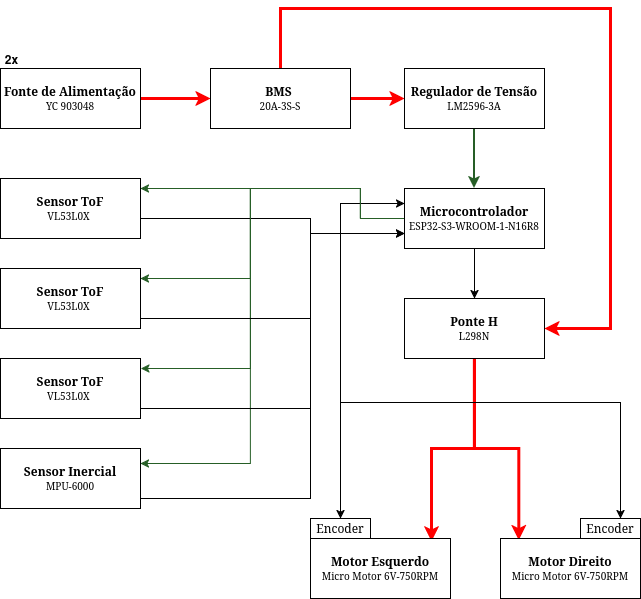
\includegraphics[width=0.8\textwidth]{figuras/diagrama_componentesFinal.png}
    \captionsetup{font=footnotesize}
    \caption{Diagrama de componentes do Micromouse. As linhas contínuas pretas representam conexões físicas via protocolo I2C. As linhas verdes representam alimentação em baixa tensão (3,3V). As linhas vermelhas representam alimentação em alta tensão (6V). As linhas tracejadas representam comunicação sem fio.}
    \label{fig:diagrama_componentes}
\end{figure}


\textcolor{red}{A Fig. \ref{fig:diagrama_blocos_e_esquematico} apresenta o diagrama de blocos e o esquemático de um circuito conversor de corrente alternada para corrente direta, a título de exemplo. Repare que o diagrama de blocos indica os subsistemas do circuito completo apresentado no esquemático.
% Comecem com o diagrama de blocos, que é mais genérico, e depois indiquem os detalhes com a lista de materiais e os esquemáticos.
}

\begin{figure}[H]
    \centering
    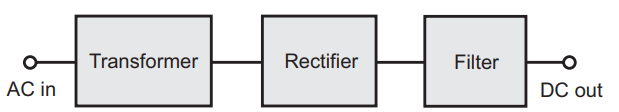
\includegraphics[width=0.5\linewidth]{figuras/Exemplo-diagrama-de-blocos.png}
    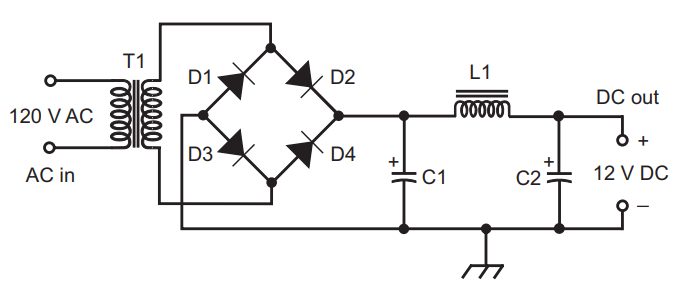
\includegraphics[width=0.5\linewidth]{figuras/Esquematico.png}
    \caption{\textcolor{red}{Diagrama de blocos e esquemático de um circuito conversor de corrente alternada para corrente direta. Extraído de \cite{block_n_schematic}.}}
    \label{fig:diagrama_blocos_e_esquematico}
\end{figure}

\section{Análise de consumo energético}

\textcolor{red}{Com relação ao consumo energético do produto desenvolvido, será necessário apresentar cálculos de consumo dos diversos componentes utilizados e explicar as decisões de projeto para atender a estas demandas.}


\begin{itemize}
    \item \textcolor{red}{ \textbf{Identificação dos Subsistemas Elétricos:} liste todos os componentes que consumirão energia, como sensores, microcontroladores, atuadores e módulos de armazenamento de dados. Para cada componente, registre a tensão de operação (V), corrente média (mA) e tempo estimado de uso (s).}
    \item \textcolor{red}{ \textbf{Cálculo da Energia Consumida por Componente:} utilize a fórmula: $E = V I t$, onde $E$ é a energia em joules, $V$ é a tensão em volts, $I$ a corrente em ampères e $t$ o tempo em segundos. Realize esse cálculo para cada componente do sistema.}
    \item \textcolor{red}{ \textbf{Estimativa do Consumo Total de Energia:} some as energias de todos os componentes para obter o consumo energético total estimado do sistema por lançamento.}
    \item \textcolor{red}{ \textbf{Escolha da Fonte de Alimentação:} com base no consumo total, converta para watt-hora: 1 Wh = 3600 J. Adicione e justifique uma margem de segurança (pesquisar o que é usual para este tipo de sistema) e selecione uma bateria ou fonte que supra a demanda.}
    \item \textcolor{red}{ \textbf{Planejamento do Circuito de Alimentação:} analise a necessidade de inclusão de reguladores de tensão, proteções contra sobrecorrente, e isolamento para atuadores. Como as oscilações de tensão serão controladas?}
    \item \textcolor{red}{ \textbf{Monitoramento via \textit{software}:} implemente, no \textit{software} embarcado, rotinas para medir a tensão da bateria e registrar dados de tempo de operação. Colete os dados para análise.}
    \item \textcolor{red}{ \textbf{Validação com Testes Reais:} realize testes de campo para comparar o consumo estimado com o real. Ajuste a capacidade da fonte se necessário e refine o software de coleta de dados. Justifique a diferença de resultados (real x teórica), de acordo com a literatura.}
\end{itemize}

\section{Descrição de \textit{software}}

\subsection{Diagrama de Atividades}

O Diagrama de Atividades (Figura \ref{fig:diagrama_atividades_sw}) descreve o comportamento funcional do sistema web do projeto XAROPi. A modelagem utiliza o particionamento por raias (\textit{swimlanes}) para estruturar o fluxo e evidenciar a fronteira entre os subsistemas da arquitetura.

Com base na notação UML, o fluxo destaca os seguintes elementos funcionais:
\begin{itemize}
    \item \textbf{Atores envolvidos:} O Estudante e o sistema físico do Micromouse.
    \item \textbf{Atividades de negócio:} Emissão de comandos de controle direcional, processamento da matriz lógica e renderização do trajeto.
    \item \textbf{Insumos (Entradas):} Ações diretas na interface pelo usuário e pacotes de telemetria transmitidos pelo ESP32 via protocolo WebSocket.
    \item \textbf{Resultados (Saídas):} Atualização dinâmica do mapa lógico na tela e a gravação final do histórico do percurso no Firebase.
    \item \textbf{Pontos de decisão:} O diagrama apresenta nós de verificação condicionais, especificamente na validação prévia de conexão estabelecida e na condição de parada automática.
\end{itemize}

O fluxo de controle se desenvolve a partir do nó de estado inicial, transitando pelas atividades assíncronas do \textit{loop} de atualização e permitindo sinais de interrupção manual pelo usuário, até o armazenamento dos dados e o atingimento do estado final.

\begin{figure}[H]
    \centering
    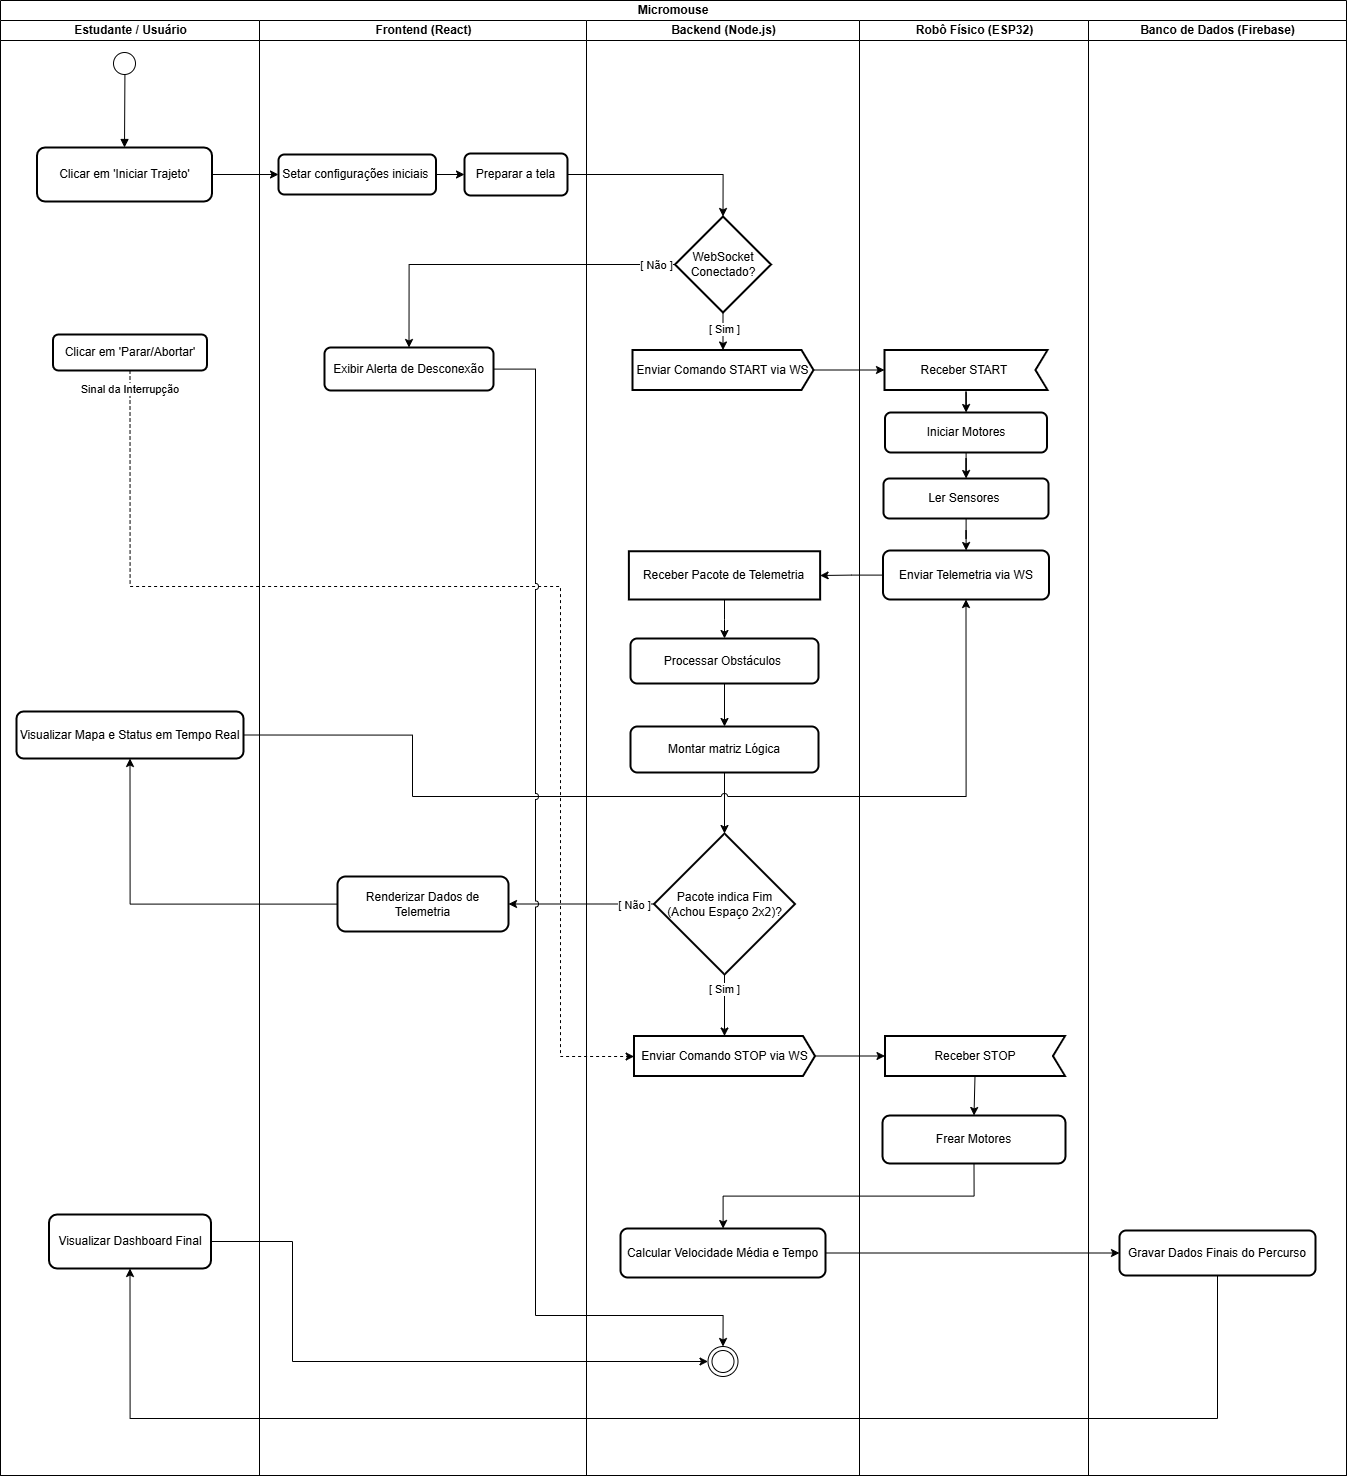
\includegraphics[height=15cm]{figuras/software/diagrama_atividades.png}
    \caption{Diagrama de Atividades de Software XAROPi.}
    \label{fig:diagrama_atividades_sw}
\end{figure}

\subsection{Backlog do Produto}

O backlog do produto é uma lista priorizada de requisitos e funcionalidades que guia o desenvolvimento do produto. Ele foi estruturado com base na EAP do projeto, (add numero da figura), e classificado utilizando a técnica MoSCoW para priorizar os requisitos e histórias de usuário. 
O backlog foi todo estruturado no github e pode ser acessado através deste \href{https://github.com/orgs/fcte-pi1/projects/8/views/1?visibleFields=%5B%22Title%22%2C274081113%2C274081114%2C%22Labels%22%2C%22Milestone%22%2C%22Assignees%22%2C%22Sub-issues+progress%22%2C%22Status%22%2C274081112%2C274081111%2C%22Linked+pull+requests%22%2C274111004%5D&hierarchy=true}{link}, onde é possivel observar com mais detalhes e compreender na sua totalidade o backlog do produto.

Na figura \ref{fig:backlog_produto} é possível observar um recorte do backlog do produto onde é possivel observar as releases, épicos, histórias de usuário e a prioriação. Além disto, cada HU está relacionada há uma parte do protótipo, ao acessar a issue específica de cada HU é possível observar na descrição. 

\begin{figure}[H]
    \centering
    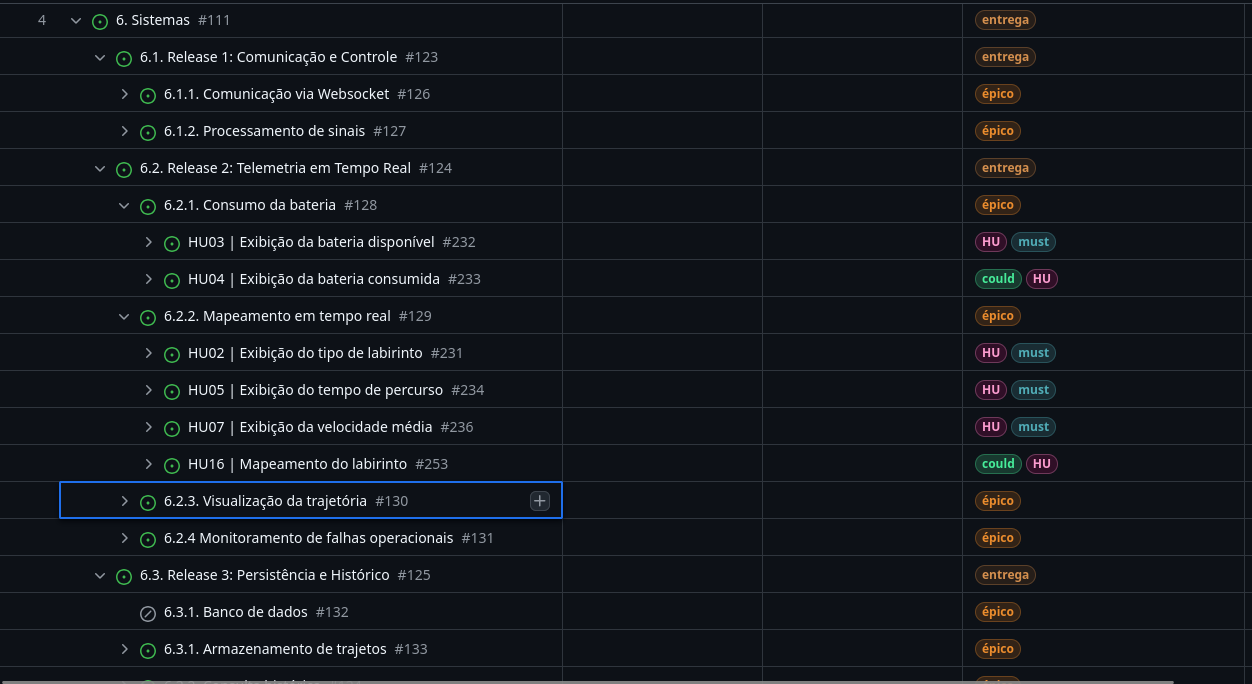
\includegraphics[width=\textwidth]{figuras/software/backlog.png}
    \captionsetup{font=footnotesize}
    \caption{Backlog do Produto (GitHub).}
    \label{fig:backlog_produto}
\end{figure}

\subsubsection{Protótipo Funcional}
O protótipo funcional foi desenvolvido com base nos requisitos funcionais que requerem apresentação e interação na interface, representados pelas Histórias do Usuário. Inicialmente, o protótipo possui duas páginas principais:
\begin{enumerate}
    \item \textbf{Página de Visão Geral:} Concentra as informações gerais de todos os testes, fornecendo métricas e gráficos importantes para uma visão holística dos testes executados. A implementação dessas funcionalidades serão essenciais para o monitoramento da evolução do projeto em uma perspectiva mais ampla Além disso, essa página também fornece uma tabela para consulta histórica dos dados de trajetos anteriores. Isso permitirá escolher quais recuperar informações de testes executados recuperar com uma visualização rápida. As HUs relacionadas a essa tela incluem: 
\href{https://github.com/fcte-pi1/2026.1_PI1_Grupo01_Bruno/issues/232}{HU03},  
\href{https://github.com/fcte-pi1/2026.1_PI1_Grupo01_Bruno/issues/233}{HU04}, 
\href{https://github.com/fcte-pi1/2026.1_PI1_Grupo01_Bruno/issues/248}{HU11}, 
\href{https://github.com/fcte-pi1/2026.1_PI1_Grupo01_Bruno/issues/249}{HU12}, 
\href{https://github.com/fcte-pi1/2026.1_PI1_Grupo01_Bruno/issues/250}{HU13}.
    \item \textbf{Página de Monitoramento em Tempo Real:} É a página a ser utilizada durante a execução de cada caso de teste. Ela exibe informações em tempo real enviadas pelo robô, como distância percorrida, obstáculos encontrados, gasto da bateria, bem como renderiza o mapa em tempo real conforme o \textit{Micromouse} o explora. Por fim, essa página também constrói e exibe gráficos como de velocidade e consumo energético. As HUs relacionadas incluem: 
\href{https://github.com/fcte-pi1/2026.1_PI1_Grupo01_Bruno/issues/230}{HU01}, 
\href{https://github.com/fcte-pi1/2026.1_PI1_Grupo01_Bruno/issues/231}{HU02}, 
\href{https://github.com/fcte-pi1/2026.1_PI1_Grupo01_Bruno/issues/234}{HU05},  
\href{https://github.com/fcte-pi1/2026.1_PI1_Grupo01_Bruno/issues/235}{HU06},  
\href{https://github.com/fcte-pi1/2026.1_PI1_Grupo01_Bruno/issues/236}{HU07}, 
\href{https://github.com/fcte-pi1/2026.1_PI1_Grupo01_Bruno/issues/237}{HU08}, 
\href{https://github.com/fcte-pi1/2026.1_PI1_Grupo01_Bruno/issues/246}{HU09},  
\href{https://github.com/fcte-pi1/2026.1_PI1_Grupo01_Bruno/issues/247}{HU10},  
\href{https://github.com/fcte-pi1/2026.1_PI1_Grupo01_Bruno/issues/251}{HU14},  
\href{https://github.com/fcte-pi1/2026.1_PI1_Grupo01_Bruno/issues/252}{HU15},  
\href{https://github.com/fcte-pi1/2026.1_PI1_Grupo01_Bruno/issues/253}{HU16};  
\end{enumerate}

\begin{figure}[H]
    \centering
    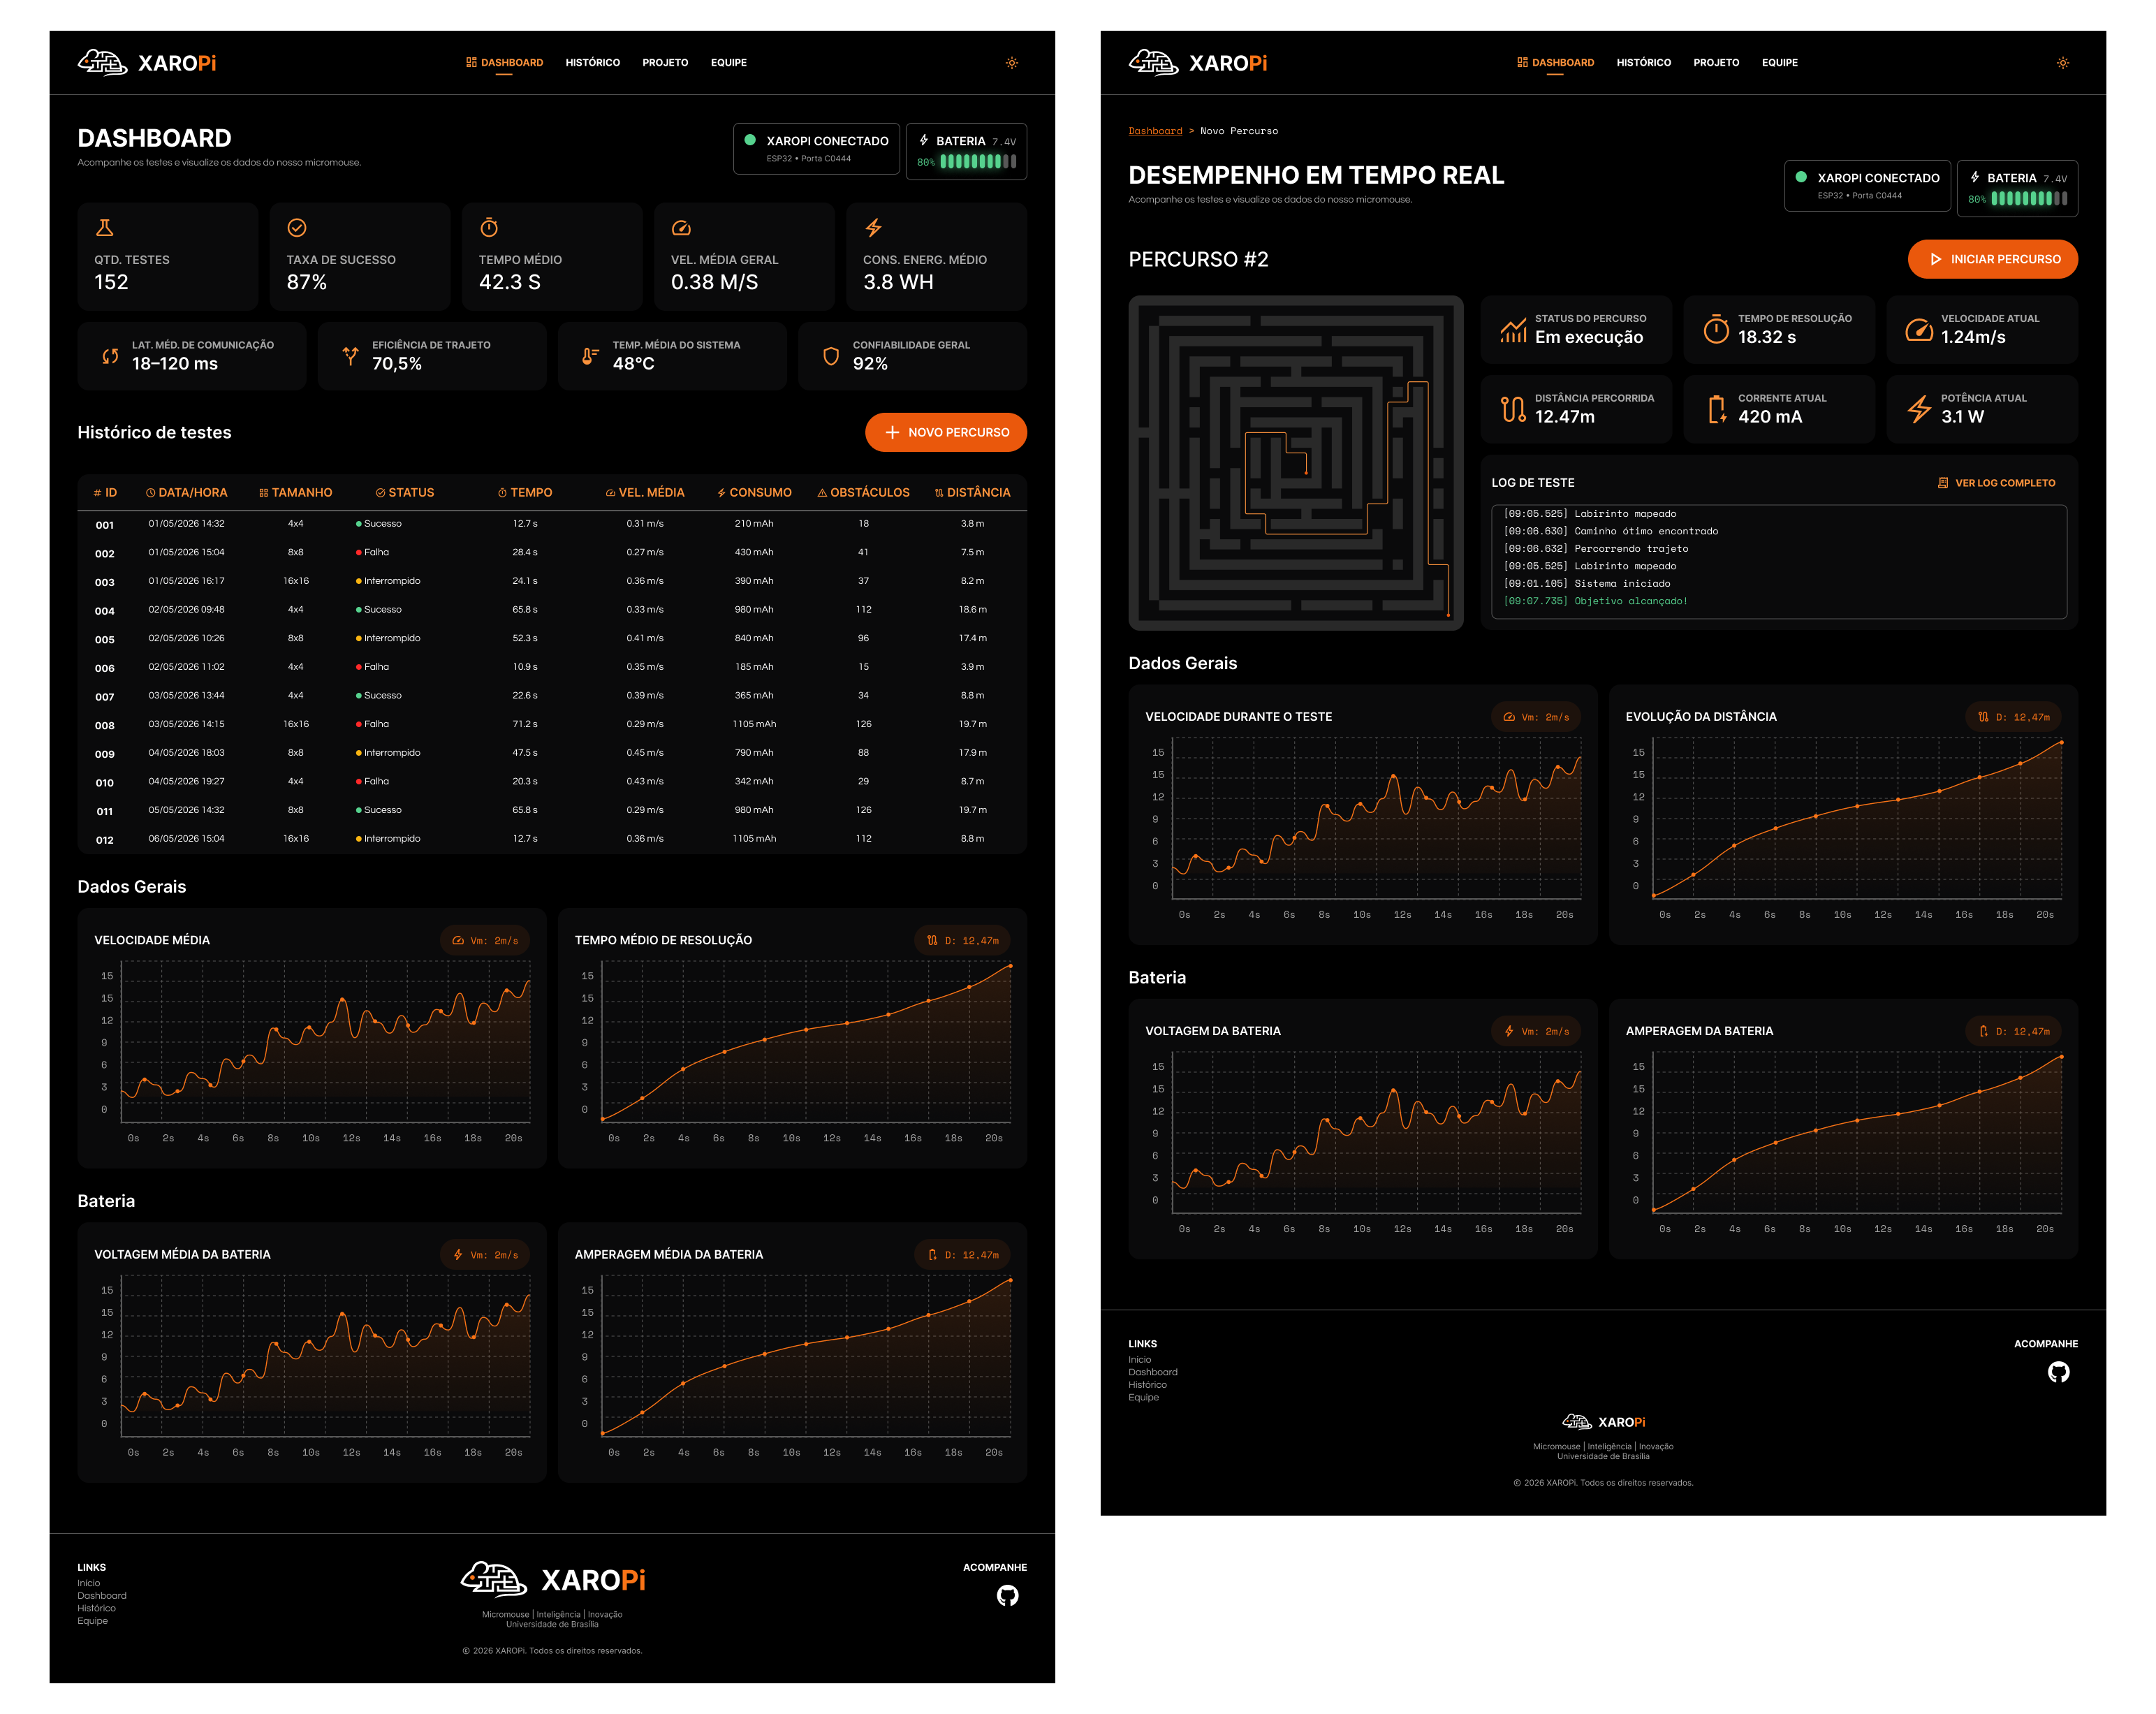
\includegraphics[width=\textwidth]{figuras/software/prototipo.png}
    \captionsetup{font=footnotesize}
    \caption{Protótipo Funcional do Sistema.}
    \label{fig:prototipo_funcional}
\end{figure}

\href{https://www.figma.com/proto/2ZyxT13T50XnVaUs51JKeb/XAROPi---Prot%C3%B3tipo-Funcional?page-id=0%3A1&node-id=46-1543&viewport=-1443%2C185%2C0.37&t=nvLNuJQbUXyazppG-1&scaling=min-zoom&content-scaling=fixed&starting-point-node-id=46%3A1543}{Link para acessar o protótipo navegável.}

\subsection{Descrição da Arquitetura do Software}

O propósito do software no projeto XAROPi é apresentar em um ambiente web e em tempo real os dados de telemetria do micromouse. Além disso, o sistema deve armazenar os dados das tentativas de resolução do labirinto e permitir consultas posteriores à finalização dos trajetos.

Para a viabilização dessas tarefas, optou-se por um modelo \textbf{monolítico em camadas}, com separação estrita entre a interface de usuário (\textit{frontend}), as lógicas de negócio (\textit{backend}) e a persistência de informações (banco de dados). A escolha pela arquitetura monolítica no lado do servidor justifica-se pela simplicidade de desenvolvimento e implantação, alinhando-se à curva de adaptação da equipe. A divisão lógica em camadas, por sua vez, garante a organização do código e facilita a manutenção.

O ecossistema do software é unificado pelo uso de \textit{JavaScript/TypeScript} e estruturado nas seguintes tecnologias e padrões:

\begin{itemize}
    \item \textbf{Interface (\textit{Frontend}):} Desenvolvida utilizando a biblioteca \textit{React}, operando com uma arquitetura orientada a componentes. A interface consome os dados do servidor e atualiza a visualização dinamicamente, separando a lógica de apresentação da lógica de processamento pesado.
    \item \textbf{Servidor (\textit{Backend}):} Construído em \textit{Node.js} com o \textit{framework} \textit{NestJS}. O \textit{backend} adota uma \textbf{Arquitetura Modular} (Controladores e Serviços), atuando como uma API que fornece dados via HTTP/REST e mantém comunicação de baixa latência com o robô via protocolo \textit{WebSocket}.
    \item \textbf{Banco de Dados:} Para o armazenamento das execuções, utiliza-se o \textit{Firebase}, um banco de dados \textit{NoSQL} orientado a documentos. Esta tecnologia permite gravar as matrizes do labirinto e tempos de percurso com alta flexibilidade e velocidade de consulta.
\end{itemize}

\subsubsection{Propósito do Software}
\subsubsection{Padrão adotado}
\subsubsection{Tecnologias escolhidas}

\subsection{Visão Lógica do Software}
\subsubsection{Diagrama de Classes}

A figura \ref{fig:diagrama_classes} apresenta o diagrama de classes do sistema, entre elas, classes para acesso ao banco de dados, para interpretação dos dados de telemetria para o frontend e para o recebimento e envio de dados com websocket. 

\begin{figure}[H]
    \centering
    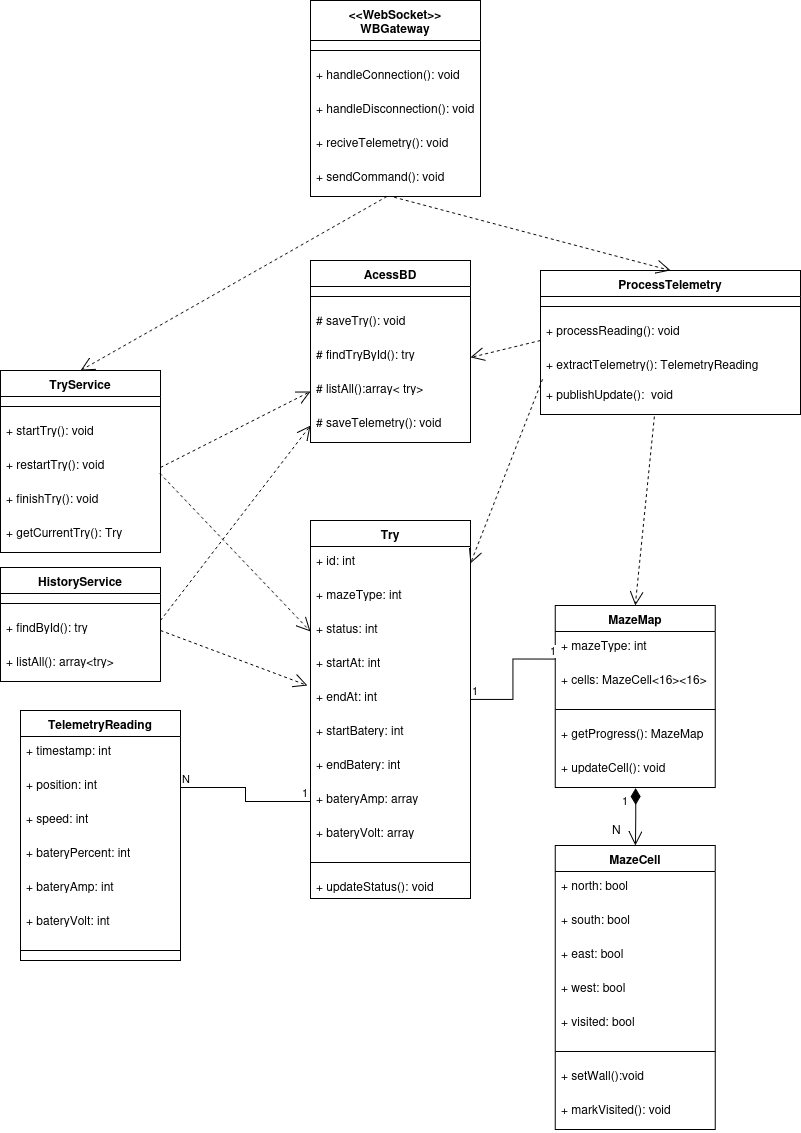
\includegraphics[height=15cm]{figuras/software/diagrama_classes.png}
    \captionsetup{font=footnotesize}
    \caption{Diagrama de Classes do Sistema.}
    \label{fig:diagrama_classes}
\end{figure}

\subsection{Visão de Processos do Software}

\subsubsection{Diagramas de Sequência}

Os Diagramas de Sequência detalham as interações temporais entre os componentes do sistema web e os agentes externos. A modelagem foca na troca de mensagens via protocolos WebSocket (tempo real) e HTTP/REST (histórico), cobrindo os fluxos críticos de operação do XAROPi.

O \textbf{Cenário de Execução Principal} (Figura \ref{fig:seq_execucao}) descreve o fluxo nominal de uma corrida. Ele demonstra a sincronização entre a interface do estudante e o hardware (ESP32), evidenciando o processamento das mensagens de telemetria e a persistência automática dos dados no Firebase ao atingir o objetivo.

\begin{figure}[H]
    \centering
    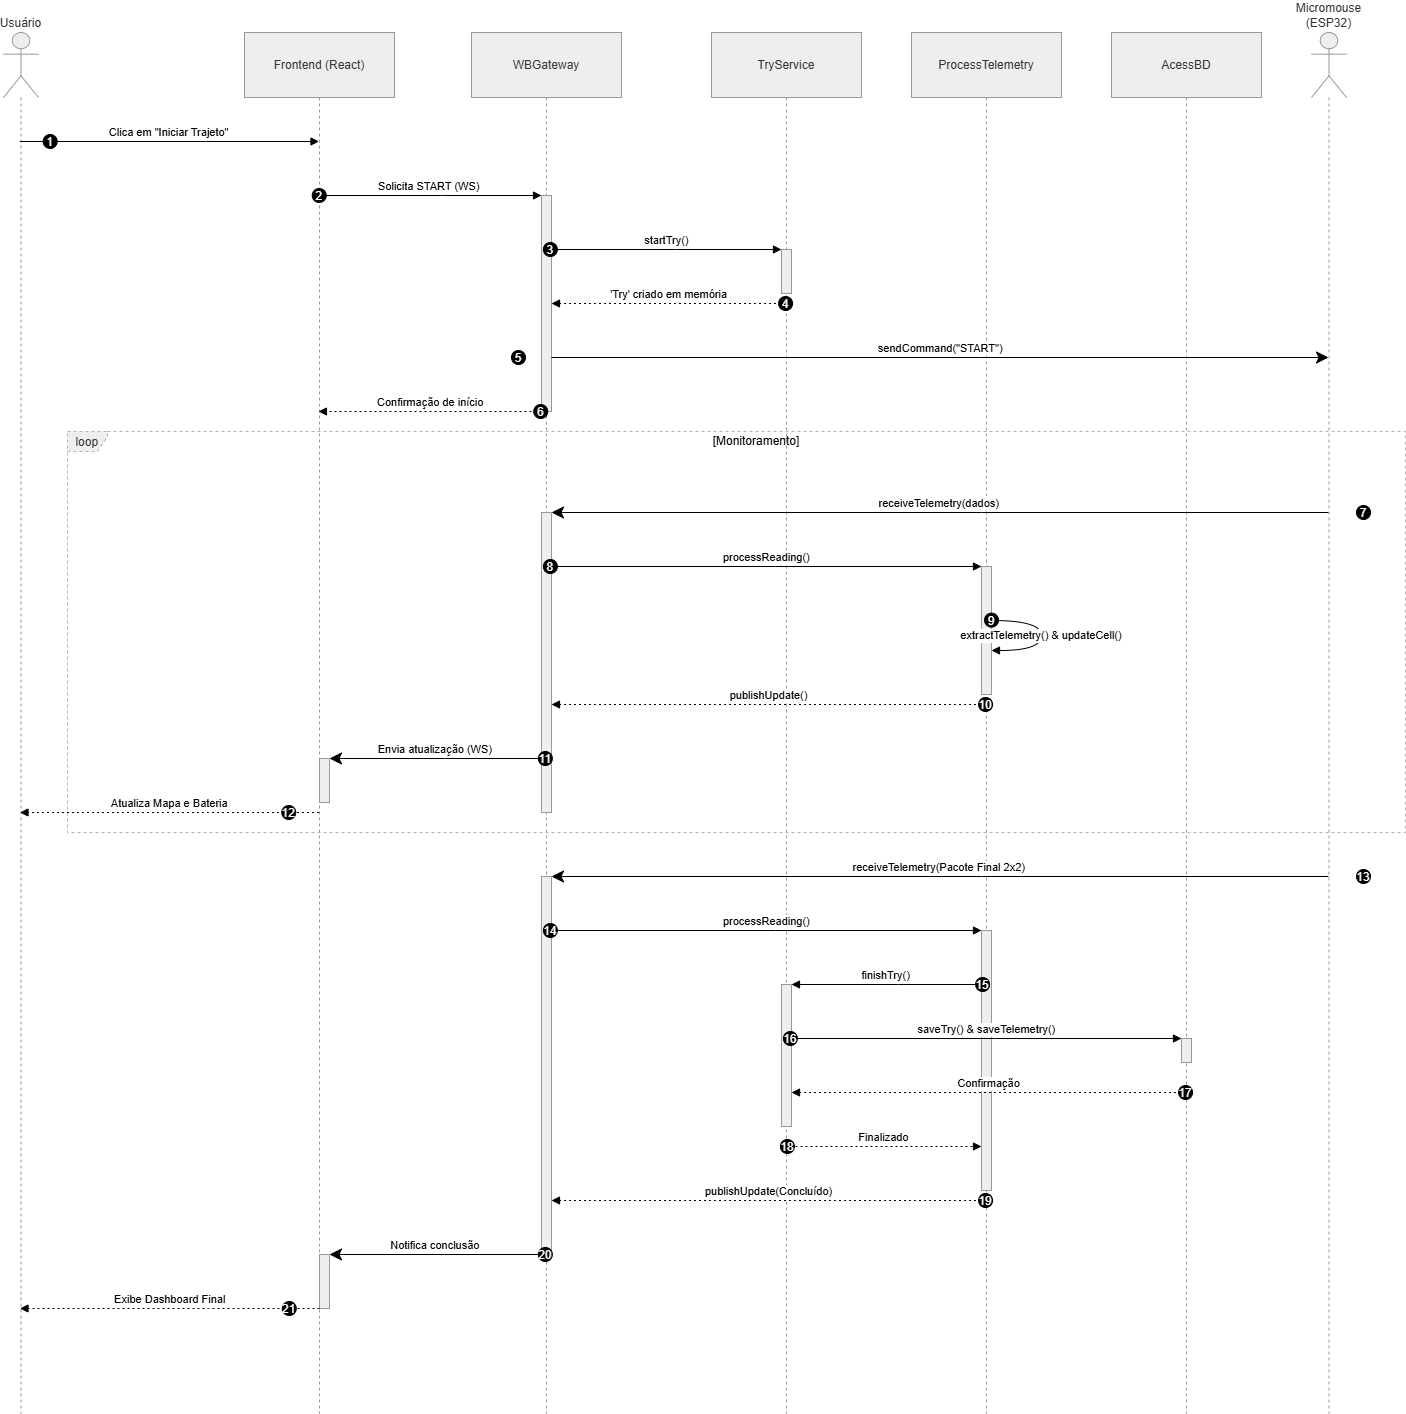
\includegraphics[width=\textwidth]{figuras/software/seq_execucao.png}
    \caption{Diagrama de Sequência: Fluxo de Execução Principal.}
    \label{fig:seq_execucao}
\end{figure}

O \textbf{Cenário de Interrupções} (Figura \ref{fig:seq_interrupcao}) mapeia a resiliência do software diante de eventos assíncronos. O diagrama ilustra o tratamento de comandos de parada manual e reinicialização enviados pelo usuário, garantindo que o estado da aplicação permaneça consistente mesmo em abortos inesperados de trajeto.

\begin{figure}[H]
    \centering
    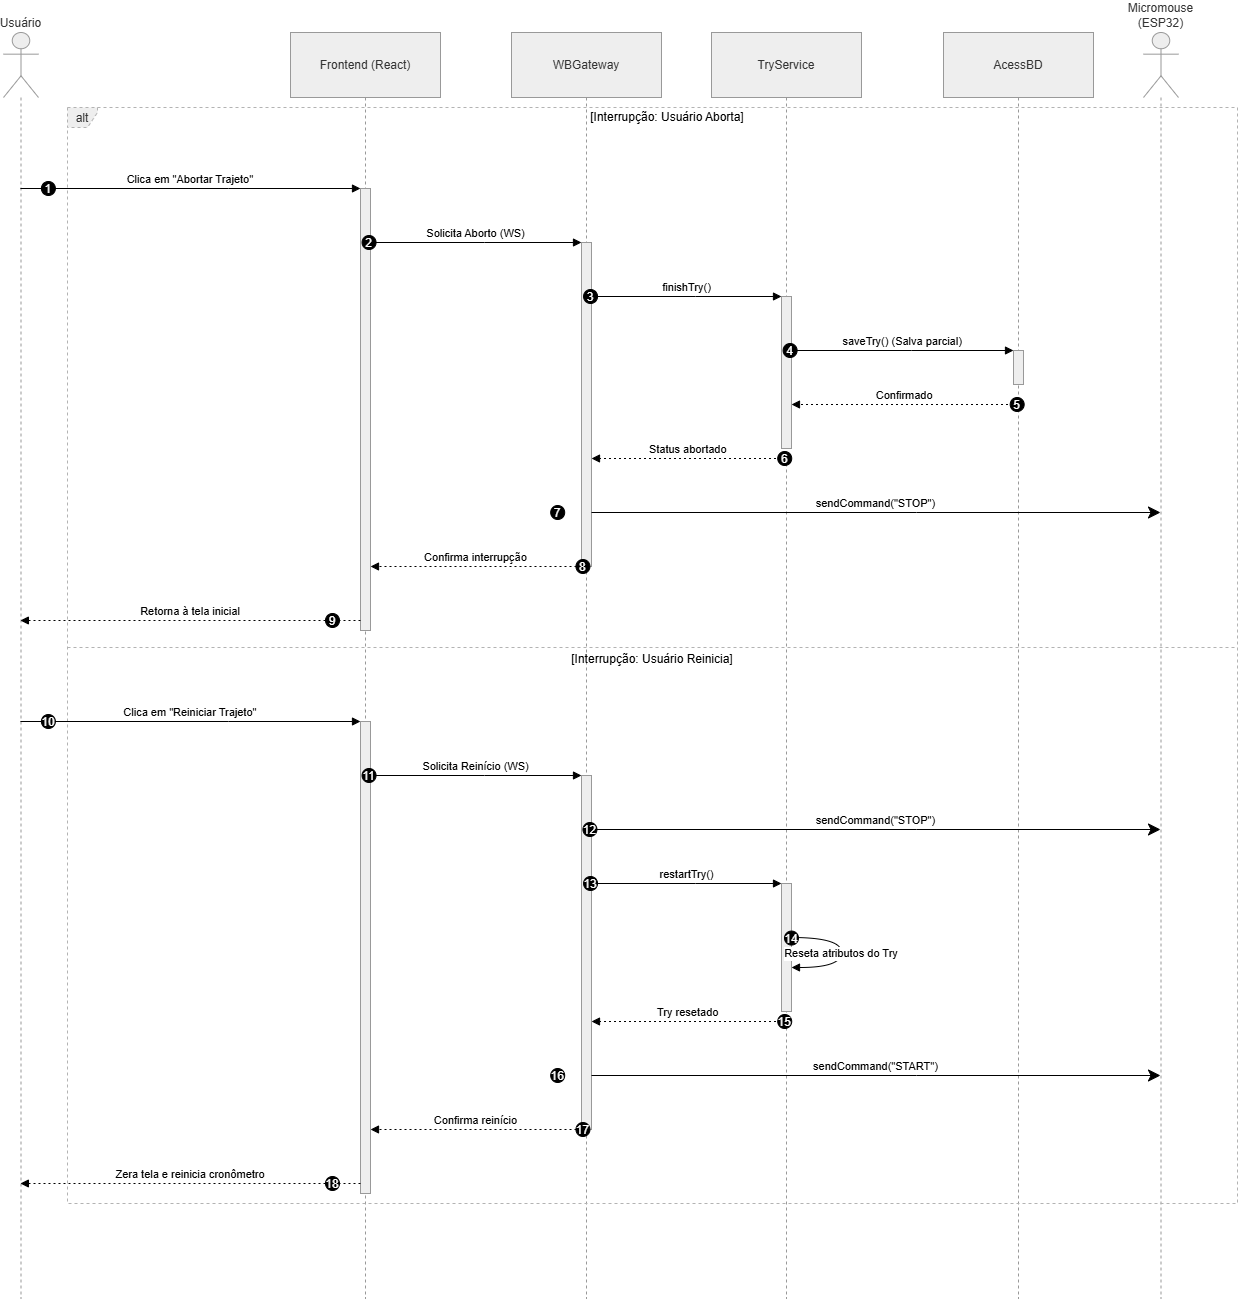
\includegraphics[width=\textwidth]{figuras/software/seq_interrupcao.png}
    \caption{Diagrama de Sequência: Fluxo de Interrupções e Resets.}
    \label{fig:seq_interrupcao}
\end{figure}

Por fim, o \textbf{Cenário de Consulta ao Histórico} (Figura \ref{fig:seq_historico}) detalha a recuperação de dados persistidos. O fluxo demonstra a comunicação entre o \textit{frontend} e o banco de dados para a renderização de trajetos passados, permitindo a análise de desempenho do robô após as corridas.

\begin{figure}[H]
    \centering
    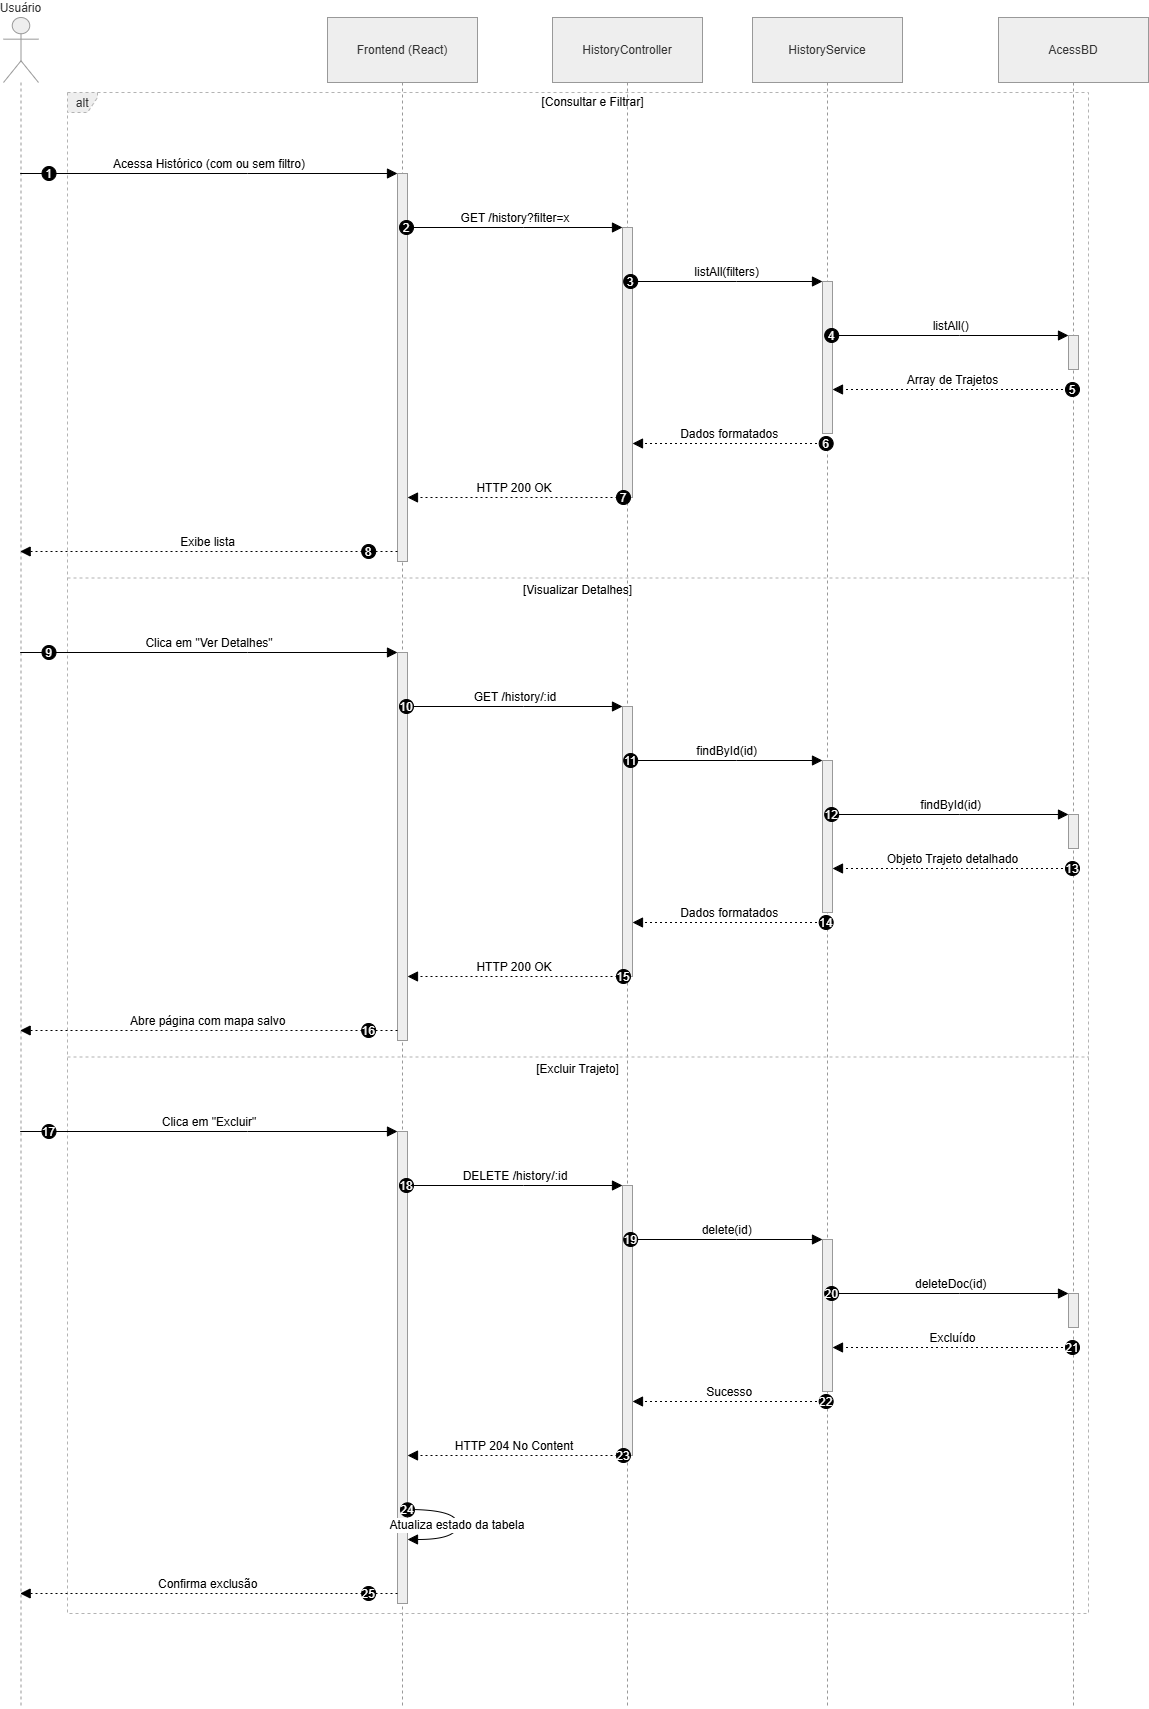
\includegraphics[width=\textwidth]{figuras/software/seq_historico.png}
    \caption{Diagrama de Sequência: Recuperação de Histórico.}
    \label{fig:seq_historico}
\end{figure}

\subsection{Visão de Implementação do Software}

\subsubsection{Diagrama de Componentes}

\subsubsection{Diagrama de Pacotes}
    O diagrama de pacotes (Figura \ref{fig:diagrama_pacotes_sw}) descreve os relacionamentos de dependência entre um pacote para outro, mostrado a disposição de cada elemento de modelo e esclarecer a estrutura hierárquia dos elementos.

    A estrutura é dividida em Frontend, representa a aplicação da interface, dividida em módulos como de componentes, lógica e comunicação, Backend, representa a comunicação entre esses dados, dividida em módulos como de telemetria e controle, EPS32, detalha o software que roda no \textit{micromouse}, dividido em módulos como de Navegação e serviço WiFi, e Firebase, que é uma camada externa utilizada para guardar os dados.
    \begin{figure}[H]
        \centering
        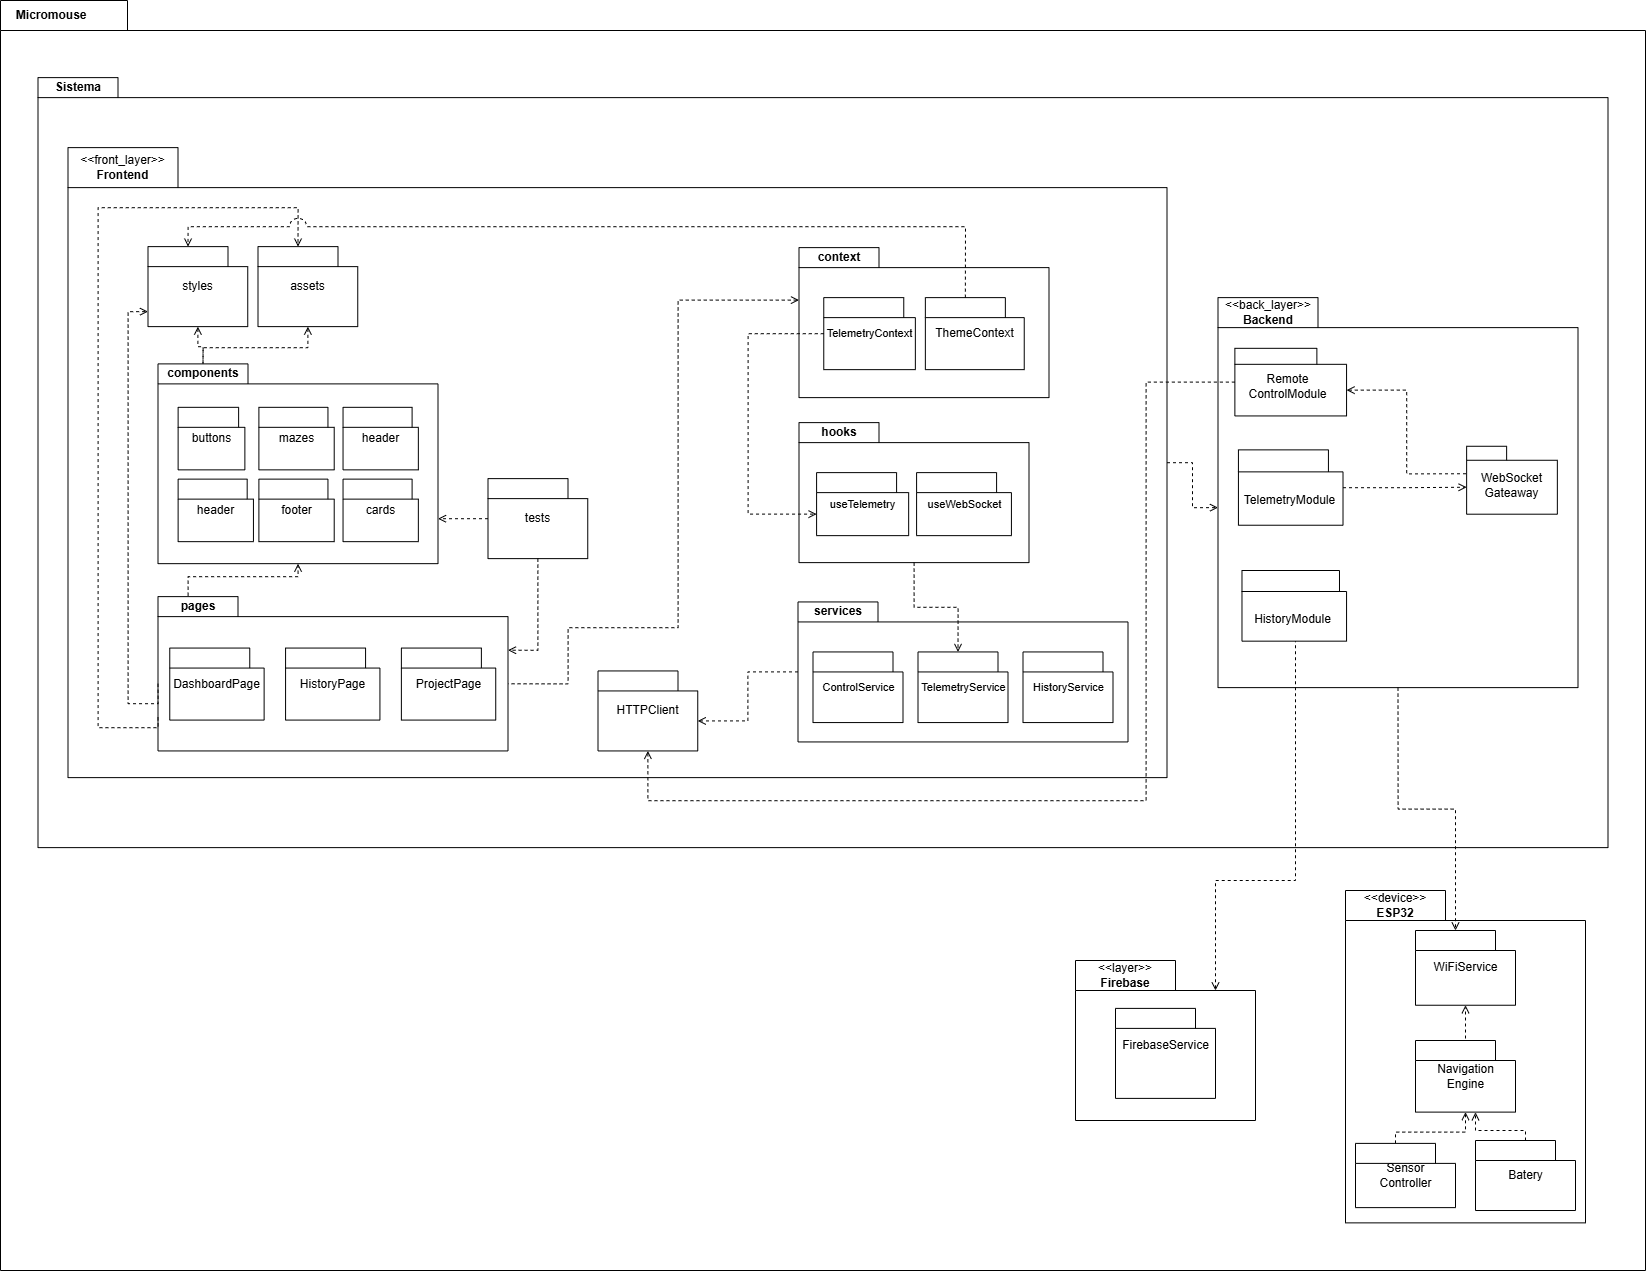
\includegraphics[width=\textwidth]{figuras/software/diagrama-de-pacotes.png}
        \caption{Diagrama de Pacotes.}
        \label{fig:diagrama_pacotes_sw}
    \end{figure}

\subsection{Visão de Implantação do Software}
\subsubsection{Diagrama de Implantação}

\begin{figure}[H]
    \centering
    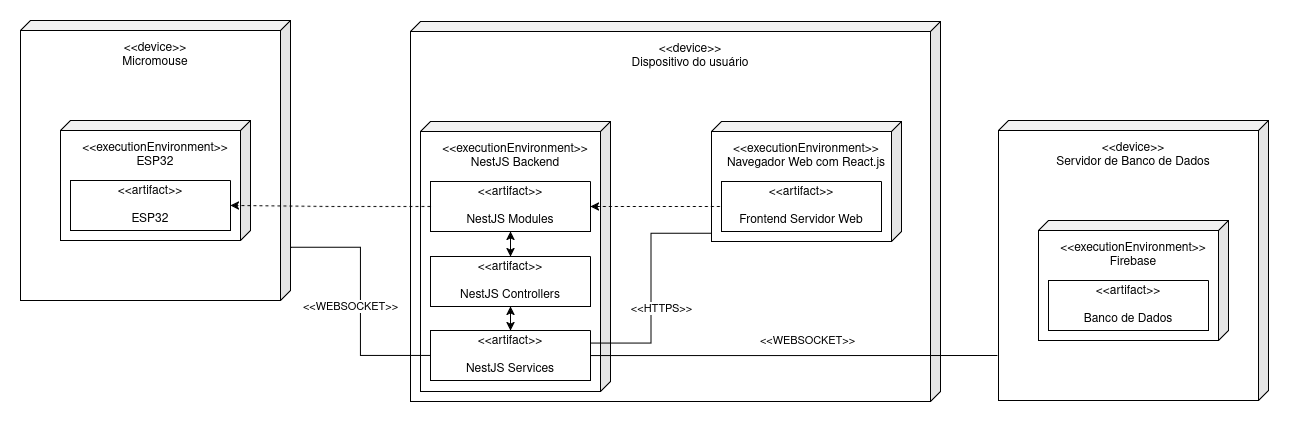
\includegraphics[width=0.8\textwidth]{figuras/software/diagrama_implantacao.png}
    \captionsetup{font=footnotesize}
    \caption{Diagrama de implantação do sistema.}
    \label{fig:diagrama_implantacao}
\end{figure}

A Fig.~\ref{fig:diagrama_implantacao} demonstra a arquitetura do sistema, caminhos de comunicação entre o \textit{Micromouse}, o sistema web, e o banco de dados, e como esses subsistemas se dispõem entre o rato físico, o dispositivo do usuário, e o serviço de banco de dados.

A comunicação entre os subsistemas acontece principalmente através de \textit{WebSocket} a fim de possibilitar o acompanhamento em tempo real da navegação do \textit{micromouse}; essa mesma razão justifica a escolha do \textbf{Firebase Realtime Database} como serviço de banco de dados. No \textit{micromouse} e back-end do servidor web, essa conexão é facilitada por módulo incluso na \textbf{ESP32} e a framework \textbf{NestJS}, respectivamente.

Como espera-se que o back-end e o front-end do servidor web sejam executados na mesma máquina (dispositivo do usuário), a conexão por \textit{HTTPS} foi determinada como suficiente para o funcionamento da interface de usuário.

O diagrama mostra também a relação de dependência entre o back-end e o \textit{micromouse} — indicando que o rato é capaz de operar independentemente — e entre o front-end e o back-end. 

\subsection{Visão de Dados do Software} 

A Visão de Dados descreve a forma como as informações geradas, processadas e consumidas pelo sistema são estruturadas e armazenadas. Tendo em vista as características do projeto, que exige alta taxa de transferência e armazenamento de dados de telemetria em tempo real, optou-se pela utilização do Firebase, um banco de dados NoSQL orientado a documentos que armazena os dados em coleções, as quais contêm documentos que podem abrigar subcoleções.

\subsubsection{Diagrama de Estrutura de Documentos} 
    Na Figura \ref{fig:diagrama_estrutura_documentos}, temos o Diagrama de Estrutura de Documentos que reflete a modelagem escolhida para otimizar as consultas do sistema web. A base de dados está dividida em duas coleções principais:

    \begin{itemize}
        \item \textbf{Coleção Labirinto:} Responsável por armazenar a estrutura física e lógica do labirinto percorrido. Cada documento representa um labirinto específico e possui atributos como \textit{id} e \textit{status}, além de uma subcoleção \textit{Nos} e uma subcoleção de metadados para dimensionamento.
        \item \textbf{Coleção Tentativa:} Responsável por armazenar o registro de telemetria do Micromouse. Cada vez que o robô inicia um percurso, um novo documento é criado nesta coleção, contendo atributos da tentativa e subcoleções específicas para os dados de velocidade e de bateria.
    \end{itemize}


    \begin{figure}[H]
        \centering
        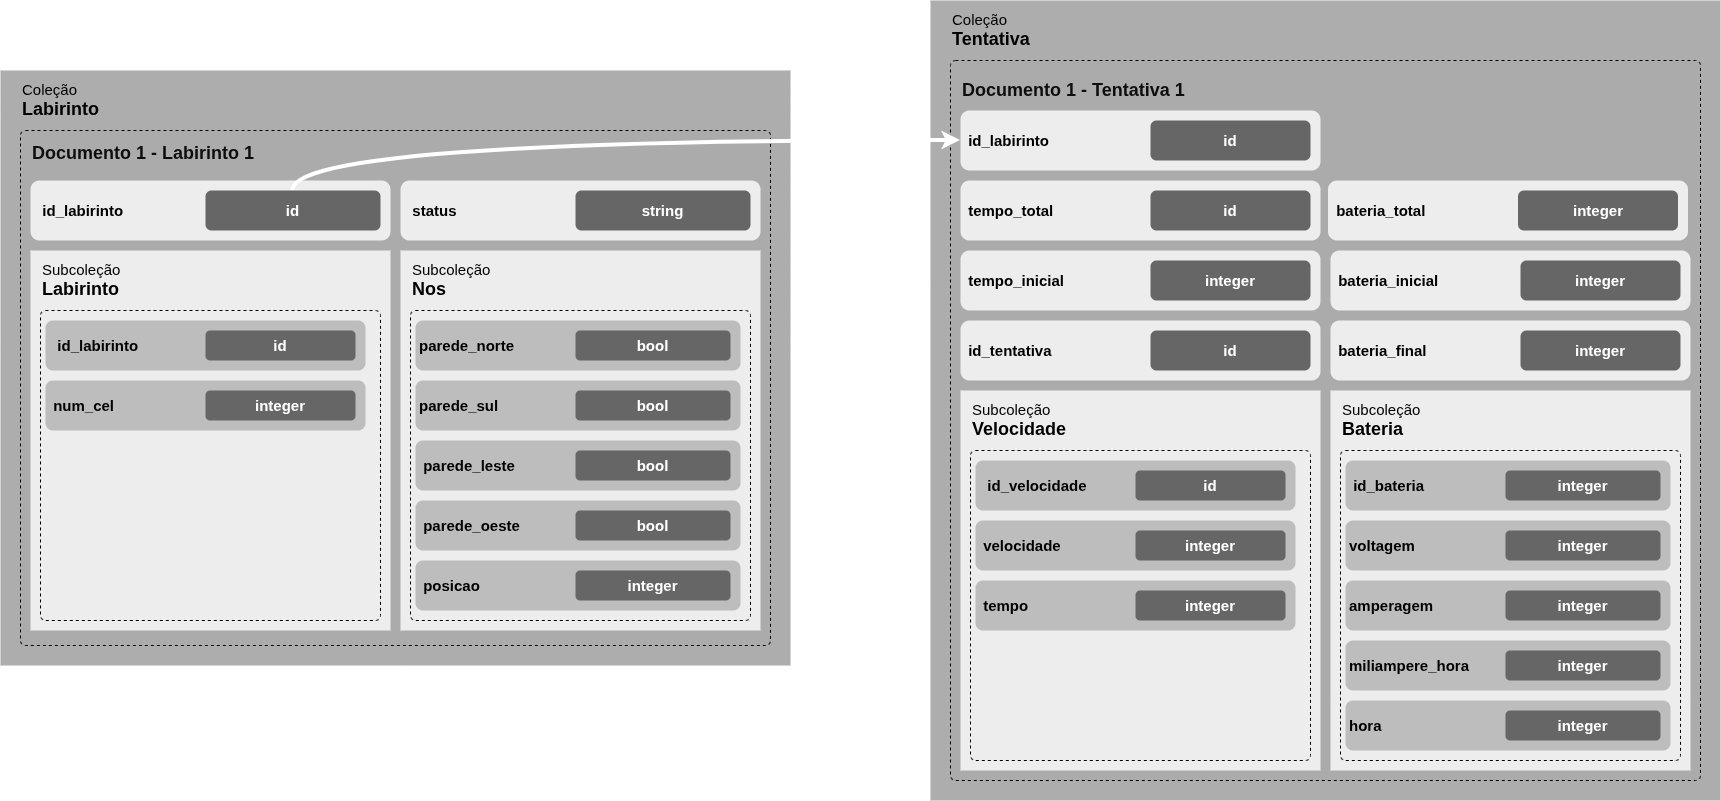
\includegraphics[width=\textwidth]{figuras/software/diagrama_estrutura_documentos.png}
        \caption{Diagrama de Estrutura de Documentos.}
        \label{fig:diagrama_estrutura_documentos}
    \end{figure}

    \subsection{Roteiro de testes funcionais}

    Os roteiro de testes funcionais pode ser observado na Tabela \ref{tab:roteiro_testes_funcionais}

    \begin{table}[H]
        \centering
        \caption{Casos de testes funcionais}
        \label{tab:roteiro_testes_funcionais}
        \footnotesize
        \begin{tabular}{|p{0.9cm}|p{2.3cm}|p{2.3cm}|p{3cm}|p{3cm}|p{3.2cm}|}
        \hline
        Id   & Nome                                & Objetivo                                                               & Pré-condições                                                                                                                                                            & Procedimentos                                                                                                                                                              & Pós-condições                                                                                                                                                                      \\ \hline
        CT01 & Monitoramento do percurso           & Validar a exibição e recebimento dos dados de telemetria do micromouse & Micromouse navegando no labirinto, servidor aberto e rodando a aplicação Web e micromouse conectado ao servidor via websocket & Iniciar o percurso e e Observar a interface web durante a execução                                                               & A interface web deve atualizar em tempo real as informações: posição no labirinto, amperagem da bateria, voltagem da bateria, velocidade, tempo da execução e status da tentativa. \\ \hline
        CT02 & Comandos remotos                    & Validar comandos remotos para o micromouse                             & Servidor aberto e rodando a aplicação Web e micromouse conectado ao servidor via websocket                                      & Apertar botão de “iniciar”, confirmar início da execução, apertar botão de “reiniciar”, confirmar reinício da execução & O sistema deve iniciar a tentativa no labirinto e o cronômetro, resetá-lo ao reiniciar.                                                                                           \\ \hline
        CT03 & Finalização e métricas da tentativa & Validar processamento dos dados ao término da tentativa                & Servidor aberto e rodando a aplicação Web, micromouse conectado ao servidor via websockete e tentativa em andamento.            & Executar a tentativa até a finalização, interrupção ou falhae e observar tela final                                              & A interface web deve informar falha/sucesso e exibir as informações médias da tentativa                                                                                           \\ \hline
        CT04 & Armazenamento de dados              & Validar o salvamento de informações após o término da tentativa.       & Servidor aberto e rodando a aplicação Web, micromouse conectado ao servidor via websockete e tentativa finalizada               & Finalizar a tentativae e consultar a tentativa no banco                                                                          & Os dados devem ser armazenados no banco de dados sem nenhuma perda de informação                                                                                                   \\ \hline
        CT05 & Consulta de histórico               & Validar consulta de tentativas anteriores.                             & Servidor aberto e rodando a aplicação Web e existência de registros salvos no banco.                                            & Pesquisar uma tentativa e clicar para visualização                                                                             & Os dados devem ser apresentados em tela sem nenhuma perda de informação para qualquer tipo de labirinto \\ \hline
        \end{tabular}
    \end{table}

    
    % \textcolor{red}{Itens fundamentais:}
    % \begin{itemize}
    %     \item \textcolor{red}{\textbf{\textit{Backlog} do Produto}}
    %     \begin{itemize}
    %         \item \textcolor{red}{ Descrever os requisitos funcionais (RF) com a técnica de documentação e especificação de história de usuário (HU);}
    %         \item \textcolor{red}{ Descrever os requisitos não-funcionais (RNF) de forma objetiva; Mais facilmente, mais rapidamente, mais responsivo, de fácil uso, são descrições subjetivas não-válidas. Um exemplo de requisito não-funcional de desempenho: ``a página deve carregar em até 5s quando em conexão 4G''.}
    %         \item \textcolor{red}{ Ao descrever os requisitos (RF e RNF), usar a classificação MoSCoW (\textit{Must have}, \textit{Should have} e \textit{Could have}), para auxiliar a priorização dos itens do backlog.}
    %         \item \textcolor{red}{ Protótipos de interface gráfica do \textit{software} em alta fidelidade.}
    %     \end{itemize}
    % \end{itemize}

    % \begin{itemize}
    % \item \textcolor{red}{ \textbf{Descrição da arquitetura da solução de \textit{software} proposta:}}
    
    %     \item \textcolor{red}{ Esta subseção deve contemplar o documento de arquitetura do sistema e deve ser estruturado segundo as visões (4+1) previstas no processo unificado (UP): lógica, de processos;  implementação, implantação e dados (substuirá a visão de casos de uso).}
        
    %     \item \textcolor{red}{ Propósito do \textit{software} (qual o seu papel no sistema);}
    %     \item \textcolor{red}{ Padrão adotado : MVC, MVP, Microsserviços, Monolítico, etc (Justificar);}
    %     \item \textcolor{red}{ Linguagens de programação: Java, Python, C\#, JavaScript, etc.}
    %     \item \textcolor{red}{ \textit{Frameworks} e bibliotecas: Spring Boot, .NET Core, React, Angular, Django, etc.}
    %     \item \textcolor{red}{ Banco de dados: Relacional (PostgreSQL, MySQL, etc) X NãoSQL (MongoDB,etc). }
    %     \item \textcolor{red}{Persistência de dados: Modelo Entidade‑Relacionamento (MER) e seu respectivo Diagrama Entidade‑Relacionamento (DER), aplicáveis quando a solução utiliza banco de dados relacional; alternativamente, diagrama de estrutura de documentos, empregado nos casos em que a arquitetura adota banco de dados não relacional.}
    % \end{itemize}  

    % \begin{itemize}
    % \item \textcolor{red}{\textbf{ Roteiro de testes funcionais:} }
    %     \item \textcolor{red}{Código do caso de teste;}
    %     \item \textcolor{red}{Nome do caso de teste;}
    %     \item \textcolor{red}{ Objetivo do caso de teste;}
    %     \item \textcolor{red}{ Pré-condições do sistema para o teste ser realizado, quando se aplicar;}
    %     \item \textcolor{red}{ Descrição dos procedimentos a serem executados para o teste;}
    %     \item \textcolor{red}{ Resultado esperado para o teste ser aprovado (pós-condição após realizado o teste);}
    % \end{itemize}
% \end{itemize}


\chapter{Orçamento}

Durante a etapa de orçamento do projeto, buscou-se minimizar os custos de forma a garantir a viabilidade financeira para todos os integrantes do grupo. Para isso, foram realizados levantamentos de preços referentes aos componentes de hardware, estrutura e consumo energético, além da matéria-prima necessária para a fabricação do chassi do micromouse e do labirinto de testes.

Houve uma redução significativa nos custos totais devido à disponibilidade prévia de alguns componentes por parte dos membros da equipe, o que nos permitiu direcionar uma parcela maior do orçamento para a aquisição de componentes com maior robustez, contribuindo para a melhoria da qualidade do projeto.

\vspace{0.5cm}

\begin{table}[htpb]
\centering
\caption{Orçamento geral.}
\begin{tabular}{|l|c|c|}
\hline
\textbf{Geral}          & \textbf{Preço previsto (R\$)} & \textbf{Preço realizado (R\$)} \\ \hline
Matéria-prima           & 84,53                         & 42,50                          \\ \hline
Componentes eletrônicos & 695,67                        & 486,04                         \\ \hline
Montagem                & 330,84                         & 317,34                          \\ \hline
\end{tabular}
\end{table}

\vspace{0.5cm}

Na tabela de orçamento por aquisição, apresentada abaixo, os componentes cujo custo real é igual a zero correspondem aos itens disponibilizados pelos integrantes do grupo.

\vspace{0.5cm}

\begin{landscape}
\begin{table}[htpb]
\centering
\caption{Orçamento por aquisição.}
\begin{tabular}{|l|l|c|c|c|}
\hline
\textbf{Item ou serviço} & \textbf{Tipo} & \textbf{Preço previsto (R\$)} & \textbf{Preço realizado (R\$)} & \textbf{Responsável} \\ \hline
Motor                    & Componente eletrônico & 151,80 & 0,00   & Gabriela \\ \hline
Sensor ToF               & Componente eletrônico & 42,45  & 61,19  & Gabriela \\ \hline
Ponte H                  & Componente eletrônico & 50,15  & 36,00   & Gabriela e Isaque \\ \hline
Giroscópio               & Componente eletrônico & 16,05  & 28,05  & Gabriela \\ \hline
Regulador de tensão      & Componente eletrônico & 7,12   & 0,00   & Gabriela \\ \hline
ESP32-S3                 & Componente eletrônico & 297,80 & 297,80 & Gabriela e Isaque \\ \hline
Rodas                    & Montagem              & 99,80  & 106,30  & Gabriela \\ \hline
MDF                      & Matéria-prima         & 84,53  & 42,50  & Isaque   \\ \hline
Bateria                  & Componente eletrônico & 67,80  & 0,00   & Gabriela \\ \hline
Chassi                   & Montagem              & 98,00  & 78,00  & Gabriela e Davi \\ \hline
Tintas                   & Montagem              & 17,64  & 17,64  & Gabriela \\ \hline
Roda boba                & Montagem              & 17,50  & 17,50  & Gabriela \\ \hline
Jumpers e barra de pinos & Componente eletrônico & 35,00  & 35,00  & João \\ \hline
Placa perfurada & Componente eletrônico & 11,40  & 11,40  & Davi \\ \hline
Insertos metálicos & Montagem & 22,90  & 22,90  & Gabriela \\ \hline
Barra de pinos & Componente eletrônico & 15,94  & 15,94  & Davi \\ \hline
Resistor e diodo & Componente eletrônico & 0,66  & 0,66  & Davi \\ \hline
Cabo de rede & Montagem & 75,00  & 75,00  & Ludmila \\ \hline
\end{tabular}
\end{table}

\begin{table}[htpb]
\begin{center}
\caption{Justificativas para itens ou serviços trocados após a aquisição.}
\begin{tabular}{|c|c|} \hline
\textbf{Item ou serviço} & \textbf{Justificativa}  \\ \hline 
   Chassi &
   Houve erros de dimensionamento nas primeiras versões. \\ \hline
   ESP32-S3 &
   Algumas ESPs foram queimadas. \\ \hline
\end{tabular}
\end{center}
\end{table}

\end{landscape}

\begin{landscape}

\chapter{Cronograma} 

% --- TABELA 1: CRONOGRAMA GERAL ---
\begin{table}[htpb]
\centering
\caption{Cronograma geral.}
\begin{tabular}{|c|c|c|}
\hline
\textbf{Geral}          & \textbf{Previsto} & \textbf{Realizado} \\ \hline
Início do projeto       & 09/04/2026        & 09/04/2026         \\ \hline
Fim do projeto          & 08/07/2026        & 08/07/2026         \\ \hline
\end{tabular}
\end{table}

\vspace{1cm}

\small 

% --- TABELA 2: CRONOGRAMA POR ATIVIDADE ---
\begin{longtable}{|p{4cm}|p{2cm}|p{2cm}|p{2cm}|p{2cm}|p{2.5cm}|p{3.5cm}|}
   \caption{Cronograma detalhado por atividade.} \label{tab:cronograma_longa} \\
    \hline
    \centering \textbf{\begin{tabular}[c]{@{}c@{}}Atividade\end{tabular}} & 
    \centering \textbf{\begin{tabular}[c]{@{}c@{}}Início\\ Previsto\end{tabular}} & 
    \centering \textbf{\begin{tabular}[c]{@{}c@{}}Início\\ Realizado\end{tabular}} & 
    \centering \textbf{\begin{tabular}[c]{@{}c@{}}Fim\\ Previsto\end{tabular}} & 
    \centering \textbf{\begin{tabular}[c]{@{}c@{}}Fim\\ Realizado\end{tabular}} & 
    \centering \textbf{\begin{tabular}[c]{@{}c@{}}Atividades\\ Prévias\end{tabular}} & 
    \centering \textbf{Responsáveis} \tabularnewline \hline
    \endfirsthead
    
    \hline
    \centering \textbf{\begin{tabular}[c]{@{}c@{}}Atividade\end{tabular}} & 
    \centering \textbf{\begin{tabular}[c]{@{}c@{}}Início\\ Previsto\end{tabular}} & 
    \centering \textbf{\begin{tabular}[c]{@{}c@{}}Início\\ Realizado\end{tabular}} & 
    \centering \textbf{\begin{tabular}[c]{@{}c@{}}Fim\\ Previsto\end{tabular}} & 
    \centering \textbf{\begin{tabular}[c]{@{}c@{}}Fim\\ Realizado\end{tabular}} & 
    \centering \textbf{\begin{tabular}[c]{@{}c@{}}Atividades\\ Prévias\end{tabular}} & 
    \centering \textbf{Responsáveis} \tabularnewline \hline
    \endhead

    \hline
    \endfoot

    \hline
    \endlastfoot

    % --- DADOS DA TABELA ---
    1 - Criação do template inicial & 09/04/2026 & 09/04/2026 & 09/04/2026 & 09/04/2026 & \multicolumn{1}{c|}{\textbf{---}} & Davi \\ \hline
    2 - Pesquisa bibliográfica sobre o tema & 09/04/2026 & 09/04/2026 & 12/04/2026 & 12/04/2026 & 1 & Todos \\ \hline
    3 - Entrega dos artefatos do PC1 & 09/04/2026 & 09/04/2026 & 11/05/2026 & 11/05/2026 & 2 & Todos \\ \hline
    4 - Desenvolvimento do software & 11/05/2026 & 11/05/2026 & 01/07/2026 & 01/07/2026 & 3 & Equipe de software \\ \hline
    5 - Escrita do PC2 & 13/05/2026 & 13/05/2026 & 08/06/2026 & 08/06/2026 & 3 & Todos \\ \hline   
    6 - Montagem do labirinto & 13/05/2026 & 20/05/2026 & 25/05/2026 & 03/06/2026 & 3 & Equipe de estrutura e Isaque \\ \hline
    7 - Validação dos componentes & 13/05/2026 & 25/05/2026 & 20/05/2026 & 01/06/2026 & 3 & Equipe de hardware \\ \hline
    8 - Montagem do veículo & 20/05/2026 & 24/05/2026 & 27/05/2026 & 25/06/2026 & 3 & Equipe de estrutura, hardware e energia \\ \hline
    9 - Montagem dos componentes & 20/05/2026 & 28/05/2026 & 25/05/2026 & 26/06/2026 & 7 & Equipe de hardware \\ \hline
    10 - Desenvolvimento do firmware & 20/05/2026 & 30/05/2026 & 04/06/2026 & 08/07/2026 & 4, 7 & Equipes de software e hardware \\ \hline
    11 - Validação do consumo energético & 08/06/2026 & 08/06/2026 & 10/06/2026 & 10/06/2026 & 7 & Equipe de hardware \\ \hline
    12 - Teste em Labirinto & 01/06/2026 & 01/06/2026 & 24/06/2026 & 08/07/2026 & 8, 9, 10 & Todos \\ \hline
    13 - Ajustes Finais & 01/07/2026 & 01/07/2026 & 08/07/2026 & 08/07/2026 & 8, 9, 10, 12 & Todos \\ \hline
\end{longtable}

\vspace{1cm}

% --- TABELA 3: JUSTIFICATIVAS ---
\begin{longtable}{|c|p{12cm}|}
    \caption{Justificativas para atrasos ou não-conclusão de atividades.} \\
    \hline
    \textbf{Atividade} & \textbf{Justificativa} \\ \hline
    \endfirsthead
    
    \hline
    \textbf{Atividade} & \textbf{Justificativa} \\ \hline
    \endhead

    \hline
    \endfoot

    \hline
    \endlastfoot

    6 - MDL & Tivemos de esperar a entrega do material, a montagem e tivemos de fazer ajustes nas dimensões. \\ \hline
    7 - VDC & A equipe de hardware tinha que esperar a conclusão do trabalho de estruturas em relação à impressão do chassi. \\ \hline
    8 - MDV & A equipe de estrutura teve de fazer algumas revisões no carrinho para adequação do peso, diminuição do tamanho e outras demandas de hardware. \\ \hline
    9 - MDC & A equipe de hardware tinha que esperar a conclusão do trabalho de estruturas em relação ao chassi. \\ \hline
    10 - DDF & A equipe de hardware teve que calibrar, recalibrar e esperar um tempo porque alguns componentes queimaram durante o período. \\ \hline
    12 - TEL & Houve atraso no término por questão de ajustes ainda feitos em algumas áreas. \\ \hline
\end{longtable}

% \normalsize 
\end{landscape}
\chapter{Testes de Verificação e Validação}

%\section{Características Gerais}

%\textcolor{red}{Introduzir os principais pontos deste capítulo. Cada teste deve %conter explicações completas que garantam sua repetibilidade:
% \begin{itemize}
%     \item Hipóteses levantadas
%     \item Condições de contorno
%     \item Resultados esperados
%     \item Materiais e métodos
%     \item Precisão e acurácia das medidas obtidas.
% \end{itemize}
%}

\section{Testes da estrutura}

Testes sobre a estrutura e versões dos protótipos do chassi e labirinto.

\subsection { Testes Estrutura e Prototipagem do Micromouse}

Para o refinamento da estrutura do Micromouse, foram fabricados por impressão 3D, utilizando materiais PETG e PLA, três versões do chassi, duas versões da tampa do compartimento da bateria e dois suportes de fixação, conforme apresentado nas Figuras~\ref{fig:prot_chassis}, \ref{fig:prot_chassis_angulo} e \ref{fig:prot_versao_final}.


\begin{figure}[htbp]
\centering
\begin{minipage}{.5\textwidth}
  \centering
  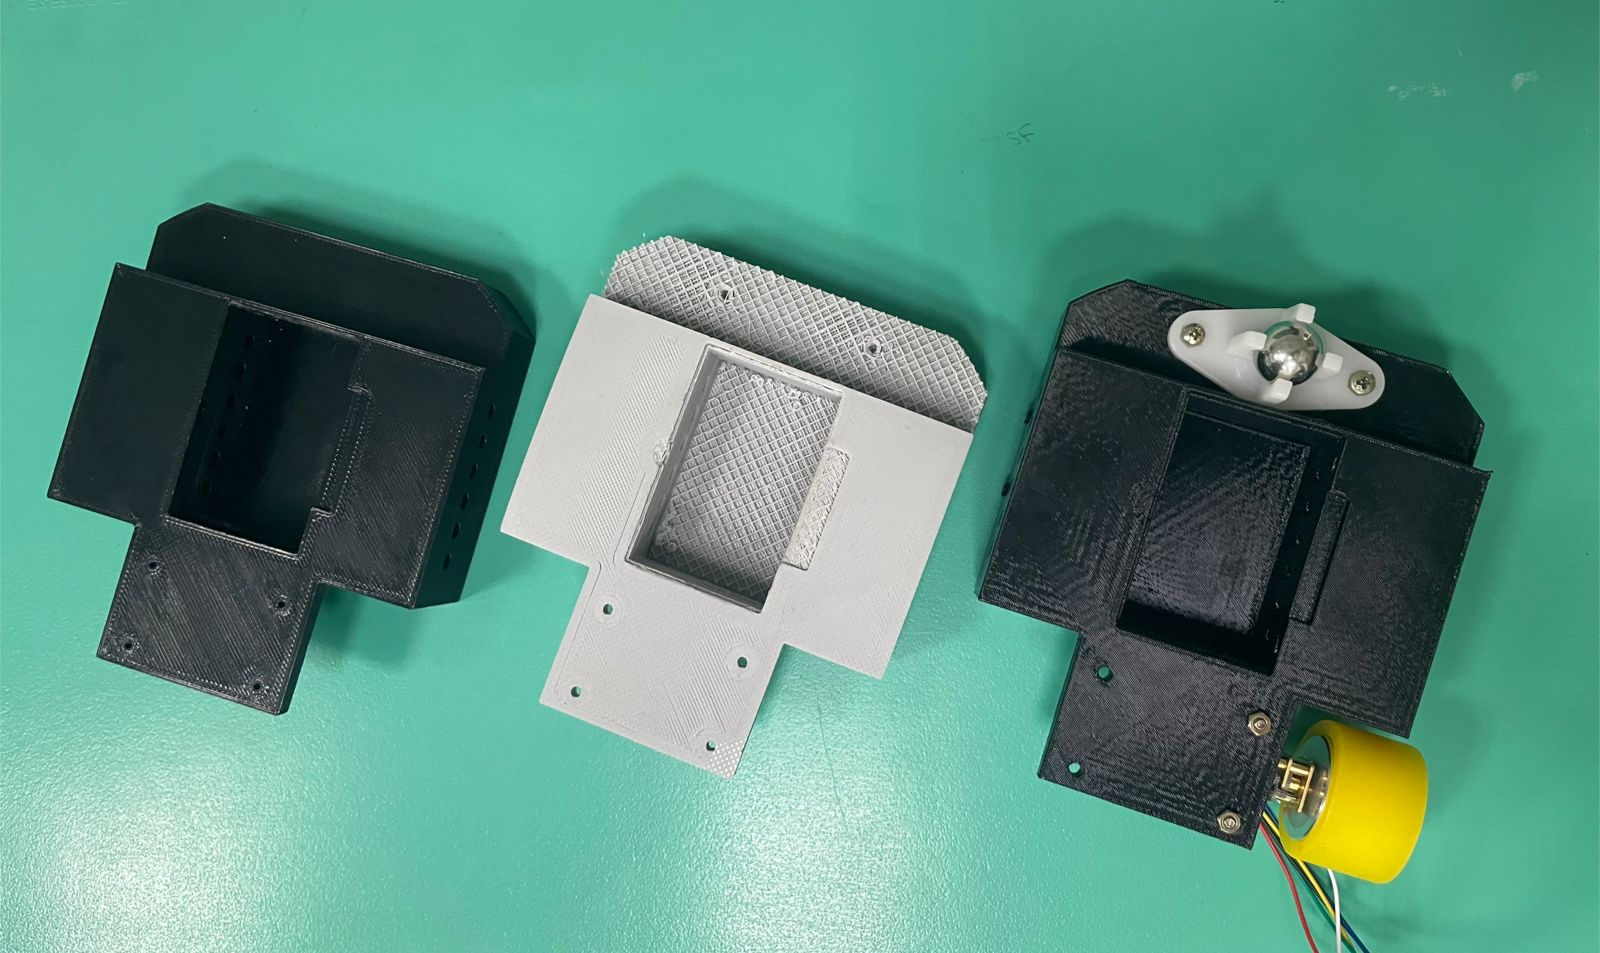
\includegraphics[width=0.7\textwidth]{figuras/versoes_chassi.jpeg}
  \captionof{figure}{Protótipos fabricados por impressão 3D.}
  \label{fig:prot_chassis}
\end{minipage}%
\begin{minipage}{.5\textwidth}
  \centering
  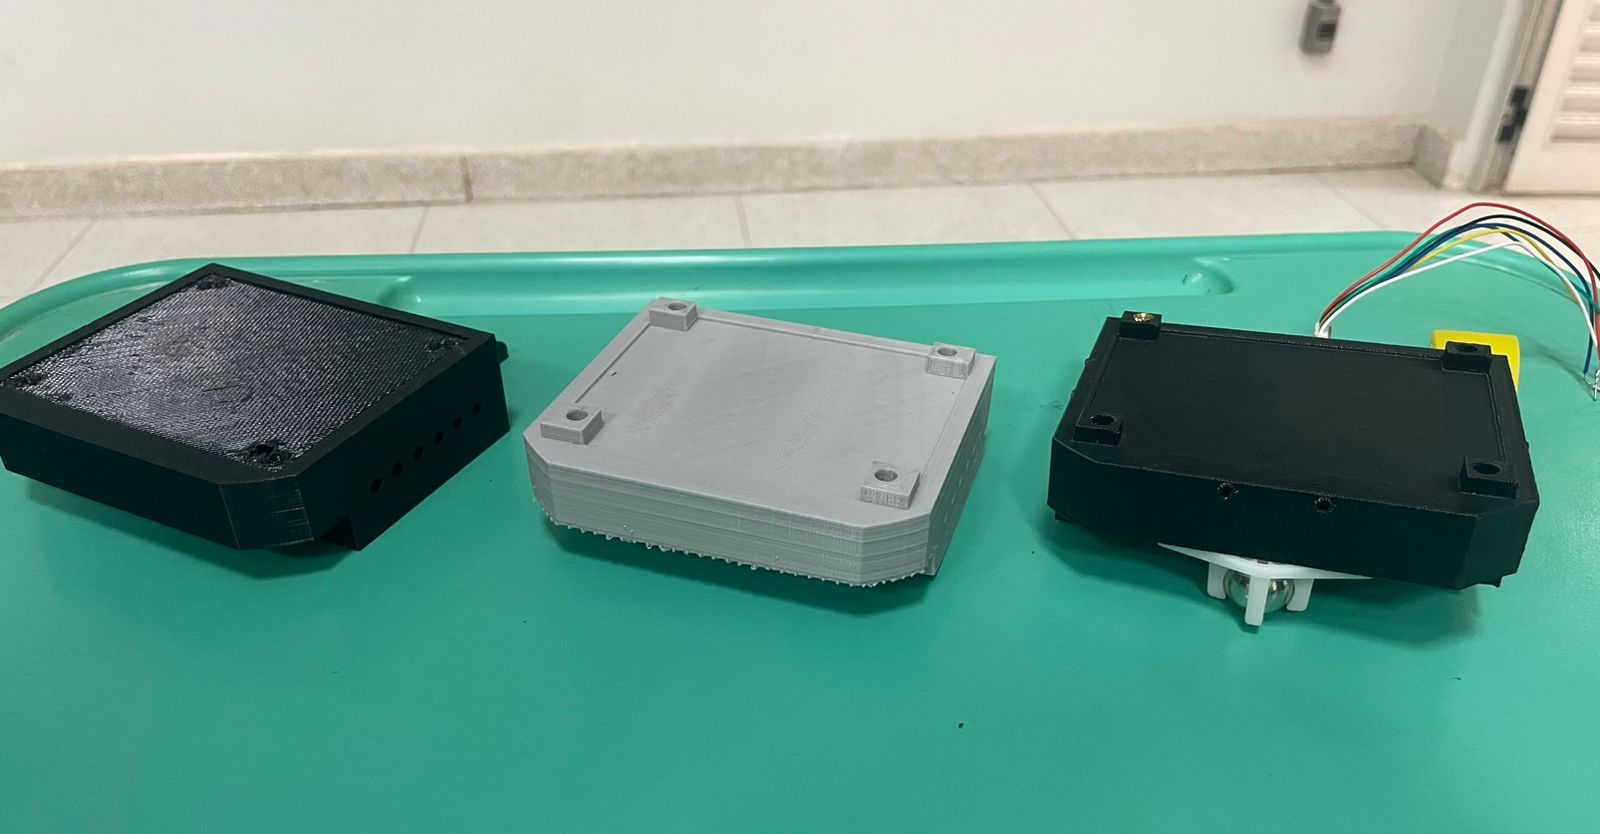
\includegraphics[width=0.7\textwidth]{figuras/versoes_chassi_angulo.jpeg}
  \captionof{figure}{Outro ângulo.}
  \label{fig:prot_chassis_angulo}
\end{minipage}
\end{figure}


Entre o projeto conceitual e a versão final, foram realizadas as seguintes modificações: ajuste dos diâmetros dos furos para compatibilidade com insertos metálicos comerciais; inclusão de ressaltos na base do sistema eletrônico para evitar interferências com componentes e pontos de solda localizados na face inferior da placa eletrônica; alteração do sistema de encaixe da tampa e reposicionamento da saída de fiação, proporcionando melhor acomodação dos cabos; realocação dos sensores ToF das laterais da placa eletrônica para as faces externas do chassi.

Essas alterações resultaram em uma melhor integração entre os componentes do sistema, contribuindo para maior robustez estrutural e facilidade de montagem.

\begin{figure}[H]
   \centering
   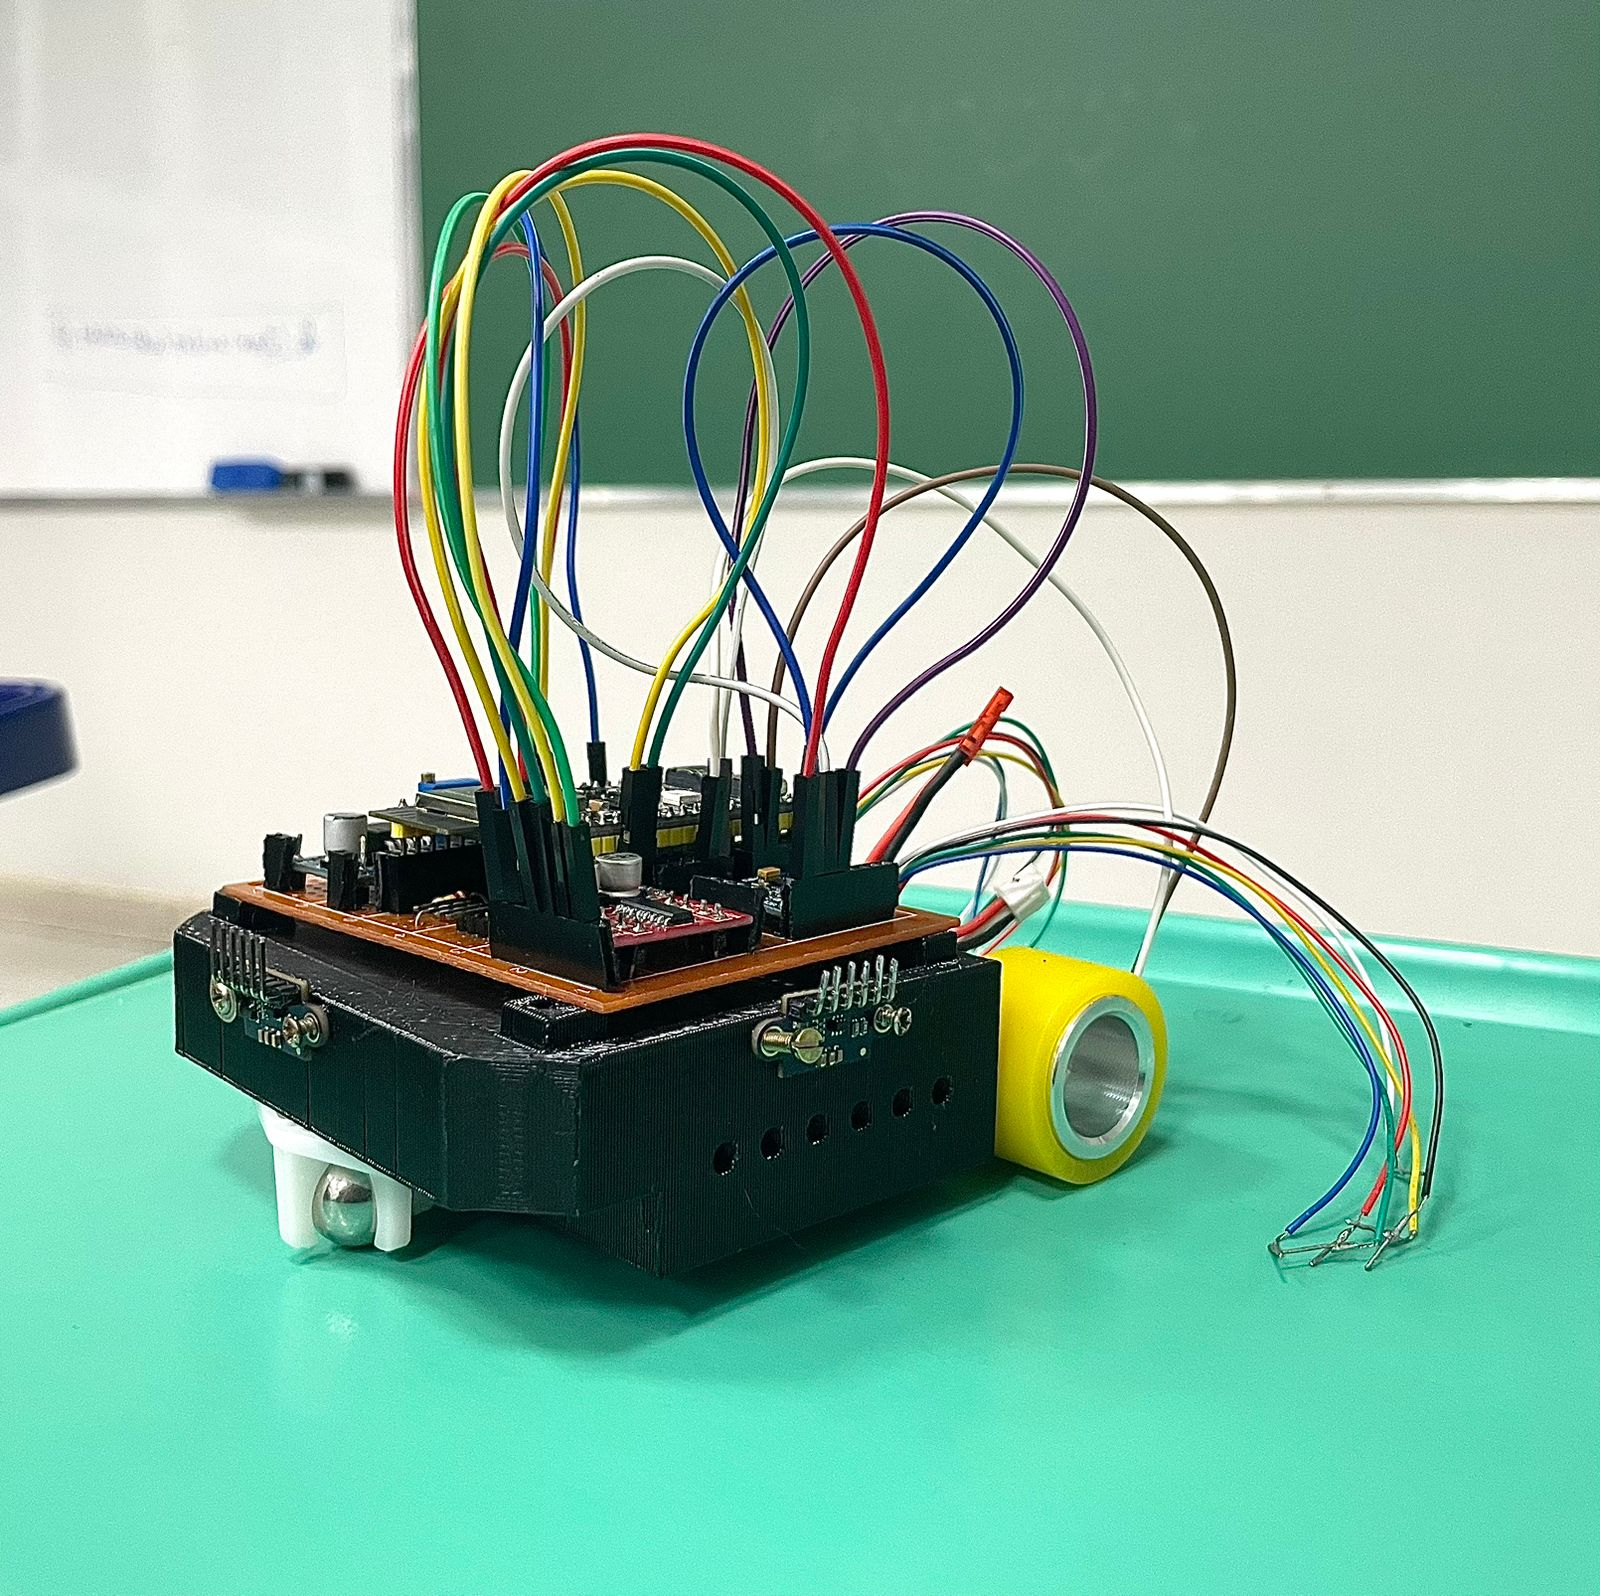
\includegraphics[width=0.45\textwidth]{figuras/versao1.2.jpeg}
   \caption{Protótipo da versão 1.2 por impressão 3D.}
   \label{fig:prot_versao_final}
\end{figure}

%\begin{figure}[H]
   % \centering
   % \includegraphics[width=0.7\textwidth]{montagem_final.jpg}
   % \caption{Montagem final do sistema Micromouse.}
   % \label{fig:montagem_final}
%\end{figure}

\subsection {Testes do labirinto}


Após a realização dos cálculos preliminares, modelagem em CAD e realização do desenho
técnico do labirinto, foi iniciada sua fabricação. As chapas de MDF foram adquiridas em
dimensões maiores do que as necessárias, sendo preciso realizar cortes para que elas se
adequassem às medidas definidas no projeto.


Durante a montagem, foi identificado um erro no dimensionamento das laterais do labirinto,
onde o cálculo inicial considerou uma parede a menos do que o necessário, resultando em
células com dimensões diferentes entre si tal como evidenciado nas Figuras~\ref{fig:montagemlabirintov1.0} e \ref{fig:labirinto}. Para corrigir o problema, optou-se por reajustar
as dimensões totais do labirinto, de modo que as paredes internas passassem a compor a
medida prevista de 18 x 18 cm para cada célula. Com essa alteração, as dimensões
externas do labirinto foram reduzidas para 72 x 72 cm. As paredes mantiveram a espessura
de 1,5 cm, conforme definido no projeto conceitual, enquanto a dimensão interna de cada
uma das 16 células passou a ser 16,125 x 16,125 cm. Dessa forma, como consta na Figura~\ref{fig:montagemlabirintov1.1}, o labirinto tornou-se
mais compacto, mas continuou atendendo aos requisitos estabelecidos para os testes.

\section{Testes de \textit{hardware}}

Seção para relato dos testes de hardware, que incluem testes de processamento, sensores, armazenamento, atuadores e comunicações.

\subsection{ESP32}
\subsubsection{\textit{Dual Core}}
Para validar o funcionamento da ESP32 e de seus dois núcleos de processamento, foi realizado um teste utilizando o FreeRTOS. A execução das tarefas foi monitorada por meio da comunicação serial, permitindo verificar a correta operação dos dois núcleos do microcontrolador. 

Foi desenvolvida uma rotina simples em que duas tarefas independentes eram atribuídas a núcleos distintos da ESP32. Cada tarefa enviava uma mensagem pela interface serial contendo a identificação do núcleo responsável pela execução. O resultado do teste é apresentado na Figura \ref{fig:teste_dualcore}. 

\subsubsection{Comunicação}
Para validar a comunicação Wi-Fi da ESP32, foi desenvolvido um algoritmo simples de conexão à rede. Durante o teste, utilizou-se uma rede Wi-Fi pessoal, cujos dados de identificação foram omitidos para preservar a privacidade dos integrantes da equipe.

Após o estabelecimento da conexão, foi realizada uma requisição HTTP ao endereço \href{http://jsonplaceholder.typicode.com/posts/1}{http://jsonplaceholder.typicode.com/posts/1}, seguida da leitura dos dados retornados pelo servidor. Após duas requisições bem-sucedidas, a conexão com a internet foi interrompida com o objetivo de verificar o comportamento do sistema e as mensagens de erro geradas na ausência de conectividade.

A Figura \ref{fig:teste_Wifi} exibe uma captura do monitor serial contendo as informações transmitidas durante o teste.

\subsection{Sensores}
\subsubsection{TOF}
Para validar os sensores TOF, foram coletados dados de distância considerando os limites estimados para a detecção de obstáculos pelo veículo. As medições foram feitas com um objeto branco fixo em frente ao sensor e as distâncias de referência adotadas foram de 80mm para o limite lateral e 50mm para o limite frontal. Durante a coleta, a posição do sensor foi mantida fixa e ajustada com o auxilio de uma régua milimetrada. Foram obtidas 403 amostras para o limite lateral e 334 amostras para o limite frontal, ambas com frequência de amostragem de 4Hz. A analise estatística dos dados coletados é apresentada na Tabela \ref{tab:tof_stats}. 

\begin{table}[h]
    \centering
       \begin{tabular}{|l|c|c|}
        \hline
        \textbf{Distância} & \textbf{Limite Lateral} & \textbf{Limite Frontal} \\ \hline
        
        \multicolumn{3}{|c|}{\textbf{Dados Gerais}} \\ \hline
        Amostras originais & 403 & 334 \\ \hline
        Outliers removidos & 0 & 1 \\ \hline
        Amostras utilizadas & 403 & 333 \\ \hline
        
        \multicolumn{3}{|c|}{\textbf{Medidas de Tendência}} \\ \hline
        Média & 81,422 & 50,928 \\ \hline
        Mediana & 81,000 & 51,000 \\ \hline
        
        \multicolumn{3}{|c|}{\textbf{Medidas de Dispersão}} \\ \hline
        Desvio padrão & 2,031 & 3,320 \\ \hline
        Coeficiente de variação (CV) & 2,494\% & 6,520\% \\ \hline
        
        \multicolumn{3}{|c|}{\textbf{Extremos}} \\ \hline
        Mínimo & 76,000 & 43,000 \\ \hline
        Máximo & 87,000 & 59,000 \\ \hline
        
        \multicolumn{3}{|c|}{\textbf{Quartis}} \\ \hline
        Q1 & 80,000 & 48,750 \\ \hline
        Q3 & 83,000 & 53,000 \\ \hline
    \end{tabular}
    \caption{Análise estatística das medições do sensor TOF para os limites lateral e frontal.}
    \label{tab:tof_stats}
\end{table}

Durante os testes, também foi observado que a distância entre os sensores e a superfície sobre a qual o micromouse navegará influencia a precisão das medições. Em alturas reduzidas, as leituras apresentaram rápido aumento de imprecisão, tendendo a valores inferiores às distâncias reais. Essa observação indica que o posicionamento dos sensores deve ser considerado durante o projeto mecânico do veículo. Registros desse comportamento podem ser encontrados nas demonstrações disponíveis no \href{https://unbbr-my.sharepoint.com/:v:/g/personal/231027079_aluno_unb_br/IQD2xGlDyRQrT7hCBopCS1RXAX4SP_C7y0wbpGJBctz3md8?nav=eyJyZWZlcnJhbEluZm8iOnsicmVmZXJyYWxBcHAiOiJPbmVEcml2ZUZvckJ1c2luZXNzIiwicmVmZXJyYWxBcHBQbGF0Zm9ybSI6IldlYiIsInJlZmVycmFsTW9kZSI6InZpZXciLCJyZWZlcnJhbFZpZXciOiJNeUZpbGVzTGlua0NvcHkifX0&e=rYLxsI}{OneDrive do projeto}. 

A partir dos dados analisados, observa-se que as leituras apresentam boa estabilidade, com pequenas variações em torno das distâncias de referência. Deve-se ressaltar que o método de posicionamento adotado introduz uma parcela de erro fixo nas medições, associada ao alinhamento manual do sensor e do objeto durante os testes. Considerando os resultados obtidos, os dados sugerem que o sensor ToF é adequado para a detecção das paredes do labirinto nas distâncias avaliadas. 

\subsubsection{MPU 6050}
Para calibração da MPU 6050, foram utilizados dois métodos: a obtenção, via média de erro de leitura, de valores de offset para cada eixo de cada sensor, e a implementação do filtro passa-baixa configurável existente no módulo via biblioteca nativa \emph{Adafruit\_MPU6050.h}. O sensor foi mantido ligado e coletou quantidades satisfatórias de dados sob as duas condições (antes e depois da calibração). Os resultados foram documentados e comparados, a fim de determinar a aplicabilidade da filtragem e frequência escolhida e dos parâmetros de offset obtidos numericamente. Os resultados das medições podem ser observados a partir dos gráficos \ref{fig:fft_acelerometro_x} a \ref{fig:fft_giroscopio_z} e da tabela \ref{tab:calibracao_mpu}.

\begin{table}[htbp]
\centering
\caption{Desvio padrão médio, mínimos e máximos em cada eixo obtidos em leitura dos dados da MPU 6050 antes e depois da aplicação dos métodos de calibração.}
\label{tab:calibracao_mpu}
\renewcommand{\arraystretch}{1.5} 
\begin{tabular}{|p{2.5cm}|p{2.8cm}|p{2.8cm}|p{2.8cm}|p{2.8cm}|}
\hline
 & \textbf{Acelerômetro (dados brutos)} & \textbf{Acelerômetro (dados tratados)} & \textbf{Giroscópio (dados brutos)} & \textbf{Giroscópio (dados tratados)} \\ \hline
\textbf{SD médio entre eixos} & 0.06827 & 0.00816 & 0.02462 & 0.00311 \\ \hline
\textbf{X mín.} & 0.59 & -0.10 & -1.17 & 0.00 \\ \hline
\textbf{Y mín.} & -1.62 & 0.02 & -0.94 & -0.01 \\ \hline
\textbf{Z mín.} & 5.19 & 9.78 & -0.41 & -0.01 \\ \hline
\textbf{X máx.} & 4.49 & 0.06 & 3.02 & 0.00 \\ \hline
\textbf{Y máx.} & 1.10 & 0.09 & 2.92 & 0.00 \\ \hline
\textbf{Z máx.} & 16.8 & 9.86 & 0.13 & 0.01 \\ \hline
\end{tabular}
\end{table}

Os dados foram coletados com o sensor parado e posicionado na horizontal, paralelo ao chão. Foi utilizada uma frequência de amostragem de 50 Hz. Os dados sem o filtro foram coletados por um tempo aproximado de 3 minutos e 19 segundos, totalizando 9950 amostras. Com o filtro passa-baixa habilitado e configurado para a frequência de 5 Hz através da função \emph{mpu.setFilterBandwidth} e o offset calculado aplicado em todos os eixos, foram coletadas um total de 6554 amostras, em um tempo aproximado de 2 minutos e 12 segundos. 

Ao analisar os gráficos e a tabela, nota-se que os dados de máximos e mínimos pós filtragem e aplicação de offset mostram-se mais concisos e coerentes com o posicionamento do sensor, pois espera-se, a partir da configuração descrita anteriormente, valores próximos de 0 em todos os eixos do giroscópio. Quanto ao acelerômetro, são esperados valores próximos de 0 em todos os eixos, com exceção do eixo Z, que, por conta da leitura da aceleração da gravidade, deve apresentar valores próximos a 9.8. Observa-se, também, uma diminuição considerável nas amplitudes e nos picos em bandas de frequência isoladas das amostras filtradas quando comparadas às amostras não filtradas. A diminuição dessa inconsistência resultou em um desvio padrão médio entre os três eixos substancialmente menor no sampling filtrado tanto no acelerômetro quanto no giroscópio, como demonstrado pela tabela \ref{tab:calibracao_mpu}. 

Os dados amostrados indicam que a aplicação dos métodos de calibração escolhidos resultaram em uma melhora significativa na confiabilidade, precisão e consistência dos dados de output da MPU 6050.

\subsubsection{Regulador de tensão e porcentagem de carga da bateria}
Para garantir uma alimentação adequada da ESP32, foi utilizado um regulador de tensão ajustável. Com o auxílio de um multímetro e da bateria prevista para o projeto, a tensão de saída foi ajustada para 5 V por meio de um trimpot, considerando a utilização do regulador interno da ESP32 DevKit. O resultado do ajuste é apresentado na Figura \ref{fig:regulador_tensao}.

Para identificar a porcentagem de carga disponível na bateria, foi utilizado um divisor de tensão conectado à entrada analógica da ESP32. O circuito também inclui um capacitor de desacoplamento, responsável pela filtragem de ruídos e pela estabilização do sinal medido. O sistema foi validado utilizando um multímetro e uma fonte de tensão contínua ajustável, permitindo observar a resposta do circuito para diferentes níveis de tensão dentro da faixa de operação prevista para a bateria do projeto. O resultado da validação é apresentada na figura \ref{fig:medidor_tensao}. 


\subsection{Atuadores}
\subsubsection{Ponte H L298N e motores DC 6V}
Uma vez que a ponte H e os motores DC 6V funcionam juntos, optou-se por realizar testes em ambos como conjunto, e não de cada um dos componentes separadamente. Os testes foram realizados via firmware com controle periódico de PWM e sentido de rotação, gravado na ESP32 conectada à ponte H. A alimentação da L298N foi feita a partir dos pinos de alimentação do devkit do microcontrolador. Os terminais de alimentação dos motores foram conectados diretamente aos terminais da bateria. 

O sistema apresentou o comportamento esperado em todas as etapas de teste. As variações de PWM, em intervalos de 50 (o argumento do PWM varia de 0 a 255), resultaram em mudanças na velocidade do motor. A mudança nos bits de sentido resultou em alteração no sentido de rotação, que, no firmware utilizado no teste, mudou a cada 2 segundos. Ambos os canais da ponte H e ambos os motores DC foram testados e avaliados, com resultados semelhantes obtidos em todos os cenários testados. Devido ao caráter qualitativo do protocolo de teste desse sistema, parte do teste foi registrado em formato de vídeo, que pode ser acessado através \href{https://unbbr-my.sharepoint.com/:f:/g/personal/231027079_aluno_unb_br/IgBTkERhmse0RpFUGiqooULzAQvzFr9VL5YGq6soeIDkyNI?e=624aZd}{deste link}.

\section{Testes de consumo energético}

Para a validação prática do dimensionamento energético, foi realizado um teste experimental com o protótipo operando pelo tempo de 20 minutos (1200 segundos). A metodologia consistiu de 10 medições de tensão ($V_k$) e corrente ($I_k$) em intervalos regulares ao longo do percurso. A partir de cada par de dados coletados, determinou-se a potência instantânea por meio do produto $P_k = V_k \cdot I_k$, gerando 10 valores distintos de potência. Na sequência, calculou-se a potência média operacional ($\bar{P}$) através da média aritmética simples dessas amostras. Por fim, esse valor médio de 15,58 W foi multiplicado pelo tempo total de operação convertido para horas ($1200/3600$ h) para a determinação da potência final consumida de 5,19 Wh. A Tabela \ref{tab:comparativo_eletrico} apresenta o comparativo entre os dados projetados no modelo teórico ideal e os dados medidos durante a validação.

\begin{table}[h!]
\centering
\caption{Comparativo de Parâmetros Elétricos (Teórico vs. Real)}
\label{tab:comparativo_eletrico}
\renewcommand{\arraystretch}{1.3}
\begin{tabular}{lcc}
\hline
\textbf{Parâmetro} & \textbf{Modelo Teórico} & \textbf{Teste Real} \\ \hline
Tensão Média Operacional & 7,40 V & 7,60 V \\ 
Potência Média & 14,15 W & 15,58 W \\ 
Energia Consumida (20 min) & 4,71 Wh & 5,19 Wh \\ 
Condição Final da Bateria & -- & 7,22 V \\ \hline
\end{tabular}
\end{table}

A bateria começou o teste com sua carga máxima de 8,4 V (tensão de pico das células Li-po 2S). Ao final do teste, a energia consumida pelo micromouse foi de 5,19 Wh, o que representou uma potência média de 15,58 W. A célula finalizou em 7,2 V.
Comparando os resultados, o consumo real foi superior ao valor teórico de 4,71 Wh devido ao torque e às perdas térmicas por efeito Joule. O consumo real permaneceu abaixo da demanda projetada com a margem de segurança estabelecida validando a escolha da bateria.

\section{Testes de \textit{software}}

Esta seção apresenta os testes realizados para verificar e validar as funcionalidades implementadas no sistema. Os testes tiveram como objetivo garantir que os requisitos definidos nas histórias de usuário foram atendidos corretamente, bem como avaliar a qualidade do código desenvolvido por meio de testes automatizados em diferentes níveis.

\subsection{Testes do algoritmo de navegação}

Para validar a lógica de navegação autônoma do robô, foram realizados testes isolados do algoritmo de \textit{Floodfill}. Tendo em vista que o processamento de navegação executará estritamente de forma local no microcontrolador (ESP32-S3), fez-se necessário garantir a corretude da lógica implementada em linguagem C para o mapeamento e otimização de rotas antes da integração com os periféricos de \textit{hardware}.

Todos os artefatos de validação encontram-se versionados na \textit{branch} \texttt{hardware} do repositório do projeto, alocados especificamente no diretório \href{https://github.com/fcte-pi1/2026.1_PI1_Grupo01_Bruno/tree/hardware/hw/docs/flood_fill/testes}{hw/docs/flood\_fill/testes}. 

Os testes contemplaram três cenários distintos, alterando as condições de contorno por meio da variação das dimensões das matrizes do labirinto. O objetivo foi avaliar não apenas o encontro do trajeto ótimo, mas também a escalabilidade e a gestão de memória do algoritmo. Para cada uma das configurações, o diretório contém o código em C utilizado para a execução e um vídeo demonstrativo comprovando o resultado:

\begin{itemize}
    \item \textbf{Cenário 4x4:} Validação da lógica base e detecção de paredes em um ambiente reduzido (arquivos \texttt{teste\_floodfill\_4x4.c} e \texttt{Teste4x4.mp4}).
    \item \textbf{Cenário 8x8:} Validação em ambiente intermediário, sendo esta a dimensão principal para os desafios de percurso estabelecidos para o projeto (arquivos \texttt{teste\_floodfill\_8x8.c} e \texttt{Teste8x8.mp4}).
    \item \textbf{Cenário 16x16:} Teste de estresse elaborado para atestar o funcionamento e a eficiência computacional da travessia em labirintos de alta complexidade (arquivos \texttt{teste\_floodfill\_16x16.c} e \texttt{Teste16x16.mp4}).
\end{itemize}

\subsection{Histórias de usuário implementadas}

Nosso projeto possui 16 histórias de usuário e durante este ponto de controle foram implementadas 13 histórias de usuário, totalizando 81\% das histórias de usuário, sendo elas listadas na tabela \ref{tab:historias} e observadas na figura \ref{fig:hus-implementadas} do protótipo. As demais histórias de usuário estão parcialmente criadas.

\begin{table}[H]
    \centering
    \scriptsize
    \caption{Histórias de usuário implementadas.}
    \label{tab:historias}
    \begin{tabular}{|l|l|}
    \hline
        \href{https://github.com/fcte-pi1/2026.1_PI1_Grupo01_Bruno/issues/246}{Hu 9 }  & Iniciar temporizador ao iniciar percurso \\ \hline
        \href{https://github.com/fcte-pi1/2026.1_PI1_Grupo01_Bruno/issues/247}{Hu 10}  & Iniciar temporizador ao reiniciar percurso \\ \hline
        \href{https://github.com/fcte-pi1/2026.1_PI1_Grupo01_Bruno/issues/252}{Hu 15}   & Identificação de obstáculos  \\ \hline
        \href{https://github.com/fcte-pi1/2026.1_PI1_Grupo01_Bruno/issues/251}{Hu 14}   & Processamento de obstáculos \\ \hline
        \href{https://github.com/fcte-pi1/2026.1_PI1_Grupo01_Bruno/issues/232}{Hu 3 }  & Exibição da bateria disponível \\ \hline
        \href{https://github.com/fcte-pi1/2026.1_PI1_Grupo01_Bruno/issues/233}{Hu 4 } & Exibição da bateria consumida  \\ \hline
        \href{https://github.com/fcte-pi1/2026.1_PI1_Grupo01_Bruno/issues/253}{Hu 16}   & Mapeamento do labirinto \\ \hline
        \href{https://github.com/fcte-pi1/2026.1_PI1_Grupo01_Bruno/issues/236}{Hu 7}   & Exibição da velocidade média \\ \hline
        \href{https://github.com/fcte-pi1/2026.1_PI1_Grupo01_Bruno/issues/234}{Hu 5}   & Exibição do tempo de percurso \\ \hline
        \href{https://github.com/fcte-pi1/2026.1_PI1_Grupo01_Bruno/issues/231}{Hu 2}   & Exibição do tipo de labirinto \\ \hline
        \href{https://github.com/fcte-pi1/2026.1_PI1_Grupo01_Bruno/issues/237}{Hu 8}   & Possuir Botão para controle remoto de operação \\ \hline
        \href{https://github.com/fcte-pi1/2026.1_PI1_Grupo01_Bruno/issues/230}{Hu 1}   & Visualização do labirinto \\ \hline
        \href{https://github.com/fcte-pi1/2026.1_PI1_Grupo01_Bruno/issues/235}{Hu 6}   & Status do desafio \\ \hline
    \end{tabular}
\end{table}

\begin{figure}[H]
    \centering
    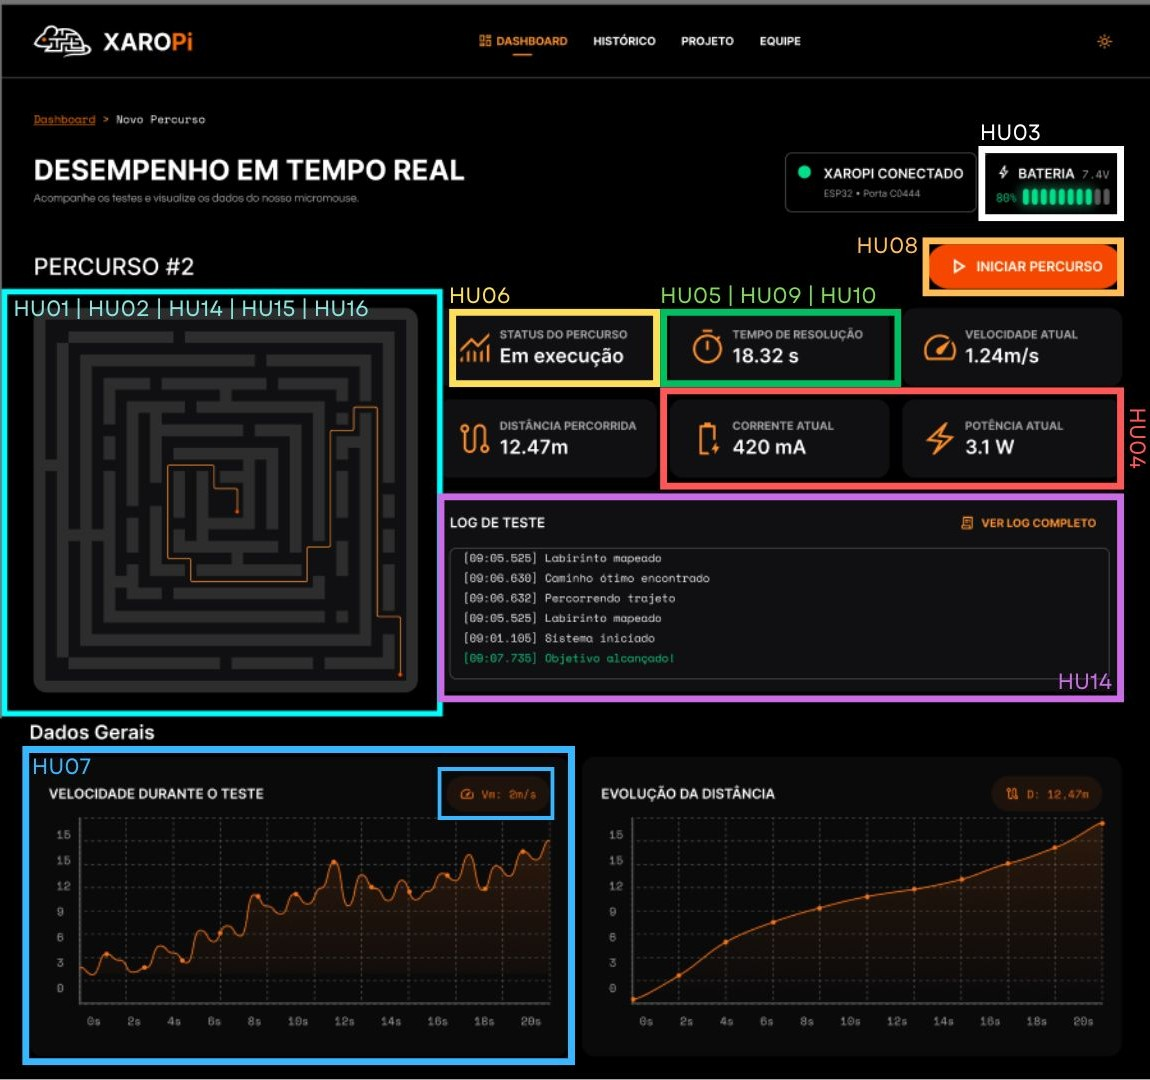
\includegraphics[width=0.65\textwidth]{figuras/software/HUsImplementadas.jpg}
    \caption{HUs implementadas apresentadas no protótipo.}
    \label{fig:hus-implementadas}
\end{figure}

\subsection{Testes unitários do frontend}

Os testes unitários do frontend foram implementados com Vitest. Foram criados testes para os seguintes componentes: badge, battery, bottomBar, breadcrumb, button, card, cell, chart, connection, controlBtn, header, log, maze, modal, tab, table e trace. O código fonte destes testes podem ser acessados em \texttt{src/frontend/src/components/nome\_componente/teste\_componente}.

Os testes verificaram a renderização dos componentes, o recebimento e a exibição correta das propriedades, o comportamento esperado em interações do usuário e a renderização condicional de elementos.

A cobertura dos testes foi analisada utilizando o Vitest. Conforme apresentado na figura \ref{fig:uni_front}, o projeto alcançou 78,37\% de cobertura de instruções e 86,36\% de cobertura de linhas, atendendo ao requisito mínimo de 70\% de cobertura de código-fonte estabelecido pela disciplina.

\begin{figure}[H]
    \centering
    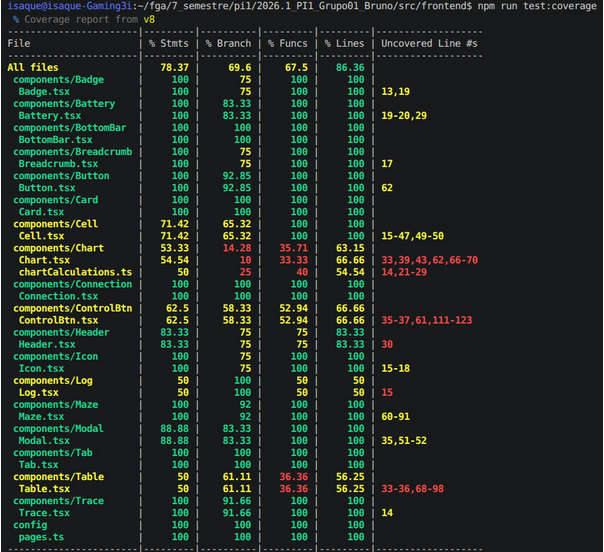
\includegraphics[width=0.7\textwidth]{figuras/software/testes_uni_front.png}
    \captionsetup{font=footnotesize}
    \caption{Relatorio de cobertura dos testes unitários do frontend.}
    \label{fig:uni_front}
\end{figure}

\subsection{Testes unitários do backend}

Os testes unitários do backend foram desenvolvidos com o objetivo de validar o comportamento individual dos serviços, controladores e gateways da aplicação, garantindo que cada módulo funcione corretamente de forma isolada. Para isso, foram utilizados testes automatizados implementados com Jest em conjunto com o módulo de testes do NestJS (\texttt{@nestjs/testing}).

Foram criadas suítes de testes para os principais módulos desenvolvidos. Os módulos contemplados pelos testes unitários são: \texttt{AppController}, \texttt{AppService}, \texttt{FirebaseService} e \texttt{TelemetryGateway}. O código fonte destes testes pode ser acessado em \texttt{src/backend/src}, nos arquivos com sufixo \texttt{.spec.ts} ao lado de cada módulo testado.

Os testes verificaram a inicialização correta dos módulos, o comportamento esperado dos endpoints HTTP, a comunicação via WebSocket com os eventos \texttt{postStart}, \texttt{postNos}, \texttt{postVelBat}, \texttt{postFinish}, \texttt{post\_posicao\_atual} e \texttt{sendcomand}, a integração com o Firebase Realtime Database, o tratamento de erros e o gerenciamento de conexões e desconexões de clientes.

A cobertura dos testes foi analisada utilizando o Jest com a flag \texttt{--coverage}. Conforme apresentado na figura \ref{fig:uni_back}, o projeto alcançou 84,14\% de cobertura de instruções e 84,11\% de cobertura de linhas, superando o requisito mínimo de 70\% de cobertura de código-fonte estabelecido pela disciplina. Os arquivos de configuração de módulos e inicialização da aplicação (\texttt{main.ts}, \texttt{app.module.ts} e \texttt{telemetry.module.ts}) foram excluídos da análise de cobertura por não possuírem lógica de negócio testável. O relatório também permitiu identificar trechos com menor cobertura, como o filtro de exceções WebSocket (\texttt{ws-exception.filter.ts}), servindo como referência para futuras melhorias nas suítes de testes.

\begin{figure}[H]
    \centering
    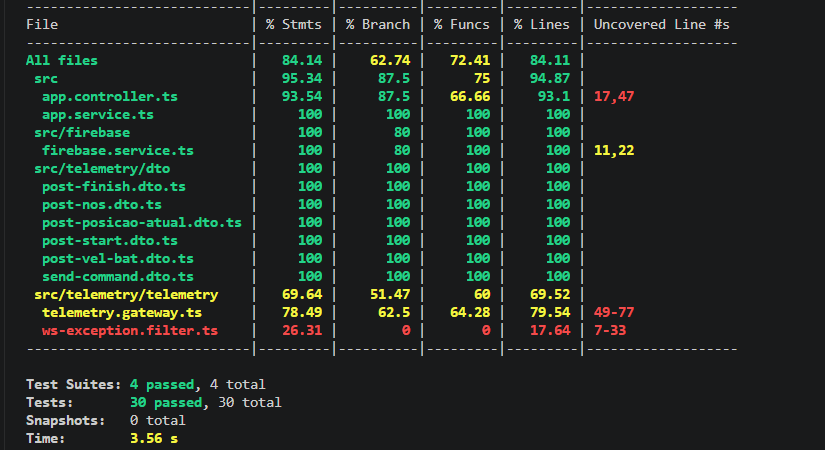
\includegraphics[width=0.7\textwidth]{figuras/software/uni_back.png}
    \captionsetup{font=footnotesize}
    \caption{Relatório de cobertura dos testes unitários do backend.}
    \label{fig:uni_back}
\end{figure}

\subsection{Testes E2E}

Foram implementados testes end-to-end utilizando Cypress com base nos roteiros de testes funcionais definidos na primeira entrega do projeto. Até o momento, foi possível implementar os casos de teste do CT1 ao CT5. O código fonte destes testes pode ser acessado em \texttt{src/frontend/src/cypress/e2e}. 

Os testes tiveram resultado positivo nos cenários CT1, CT2, CT4 e CT5. O CT3 apresentou falha por não exibir o resultado concluído na tela ao finalizar o percurso com sucesso, entretanto envia os dados corretamente para o banco.

\subsubsection{Caso de Teste 04 (CT4): Consulta de Histórico}
O CT4 tem como objetivo validar o carregamento e a renderização da tabela de histórico de percursos. O teste automatizado navega até a rota correspondente, intercepta a requisição da API e verifica se os registros antigos estão sendo listados sem perda de informação.

\begin{figure}[H]
    \centering
    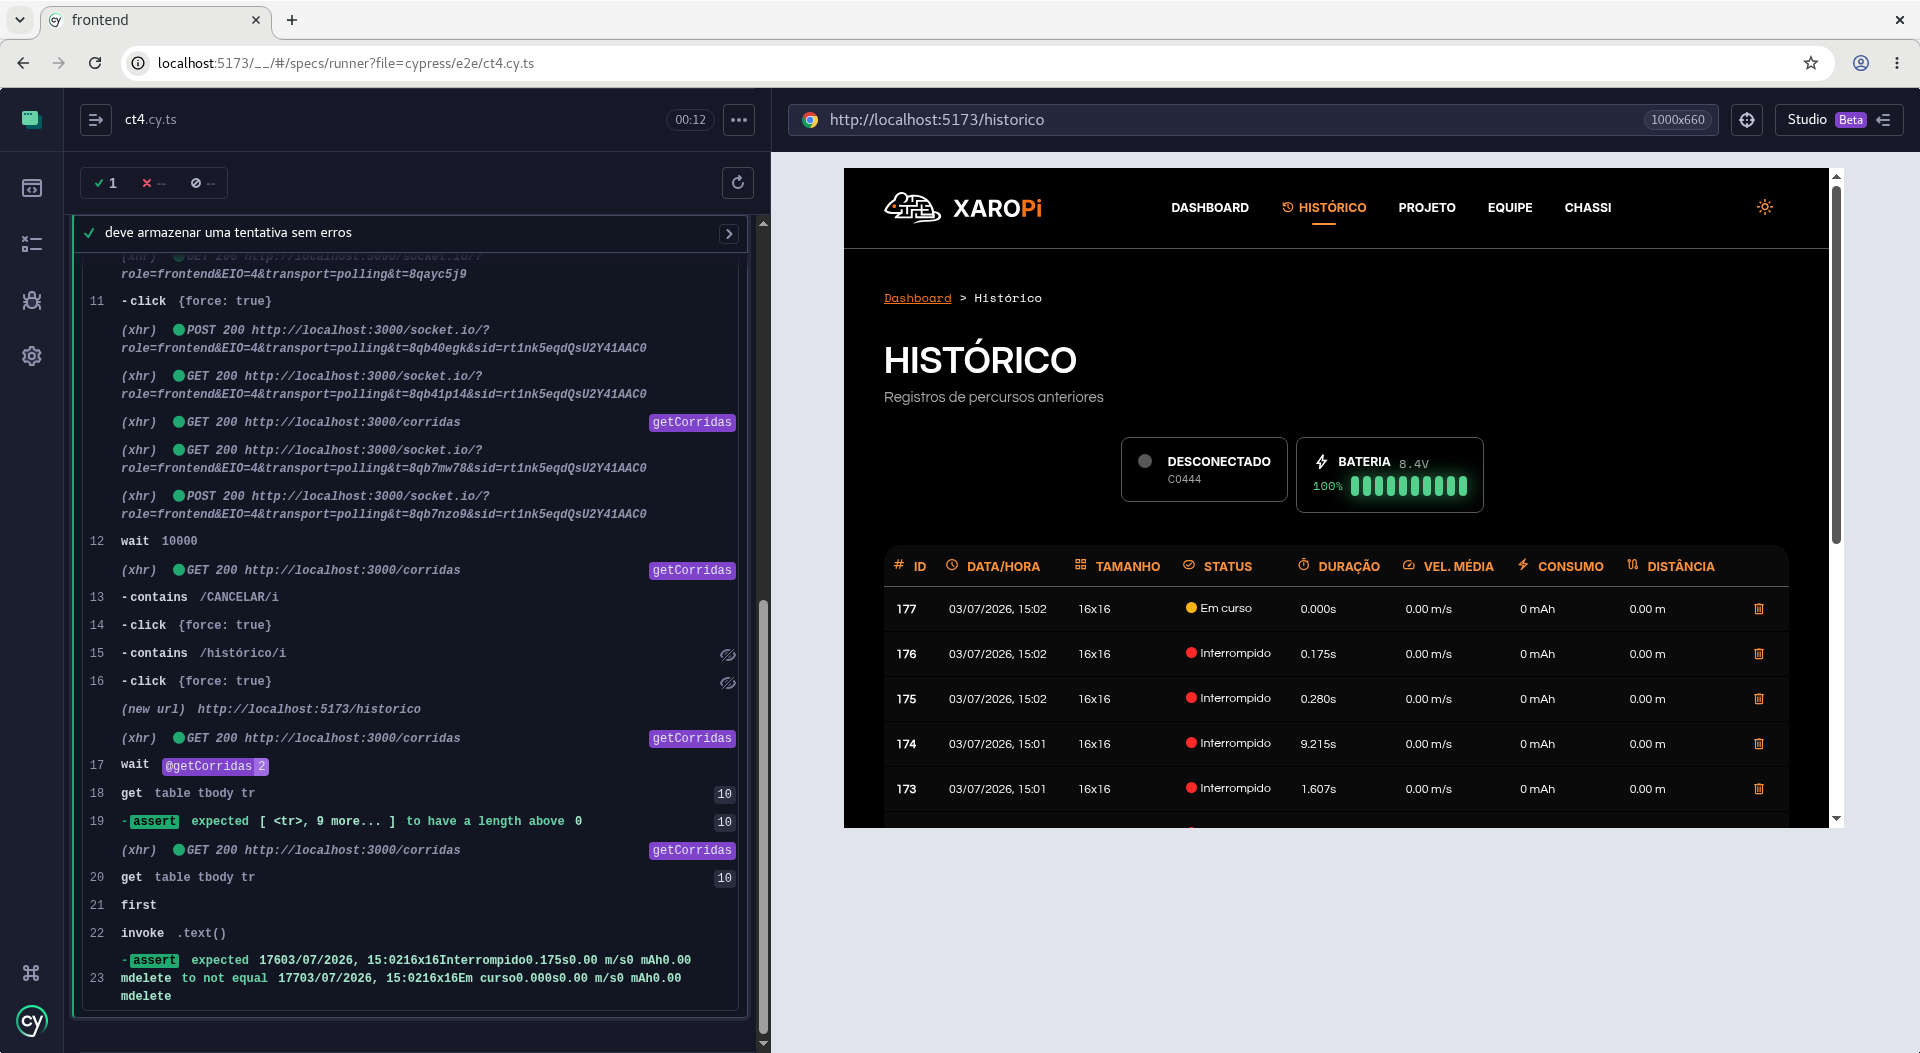
\includegraphics[width=0.9\textwidth]{figuras/software/ct4_cypress.png} 
    \caption{Execução do Caso de Teste 04 aprovada no Cypress Runner.}
    \label{fig:ct4_cypress}
\end{figure}

\subsubsection{Caso de Teste 05 (CT5): Visualização de Percurso Específico}
O CT5 avança no fluxo do histórico, testando a funcionalidade de inspecionar uma corrida passada. O Cypress valida se, ao acessar a página de detalhes, os dados gerais do percurso, bem como os gráficos de telemetria, são exibidos de forma correta e síncrona.

\begin{figure}[H]
    \centering
    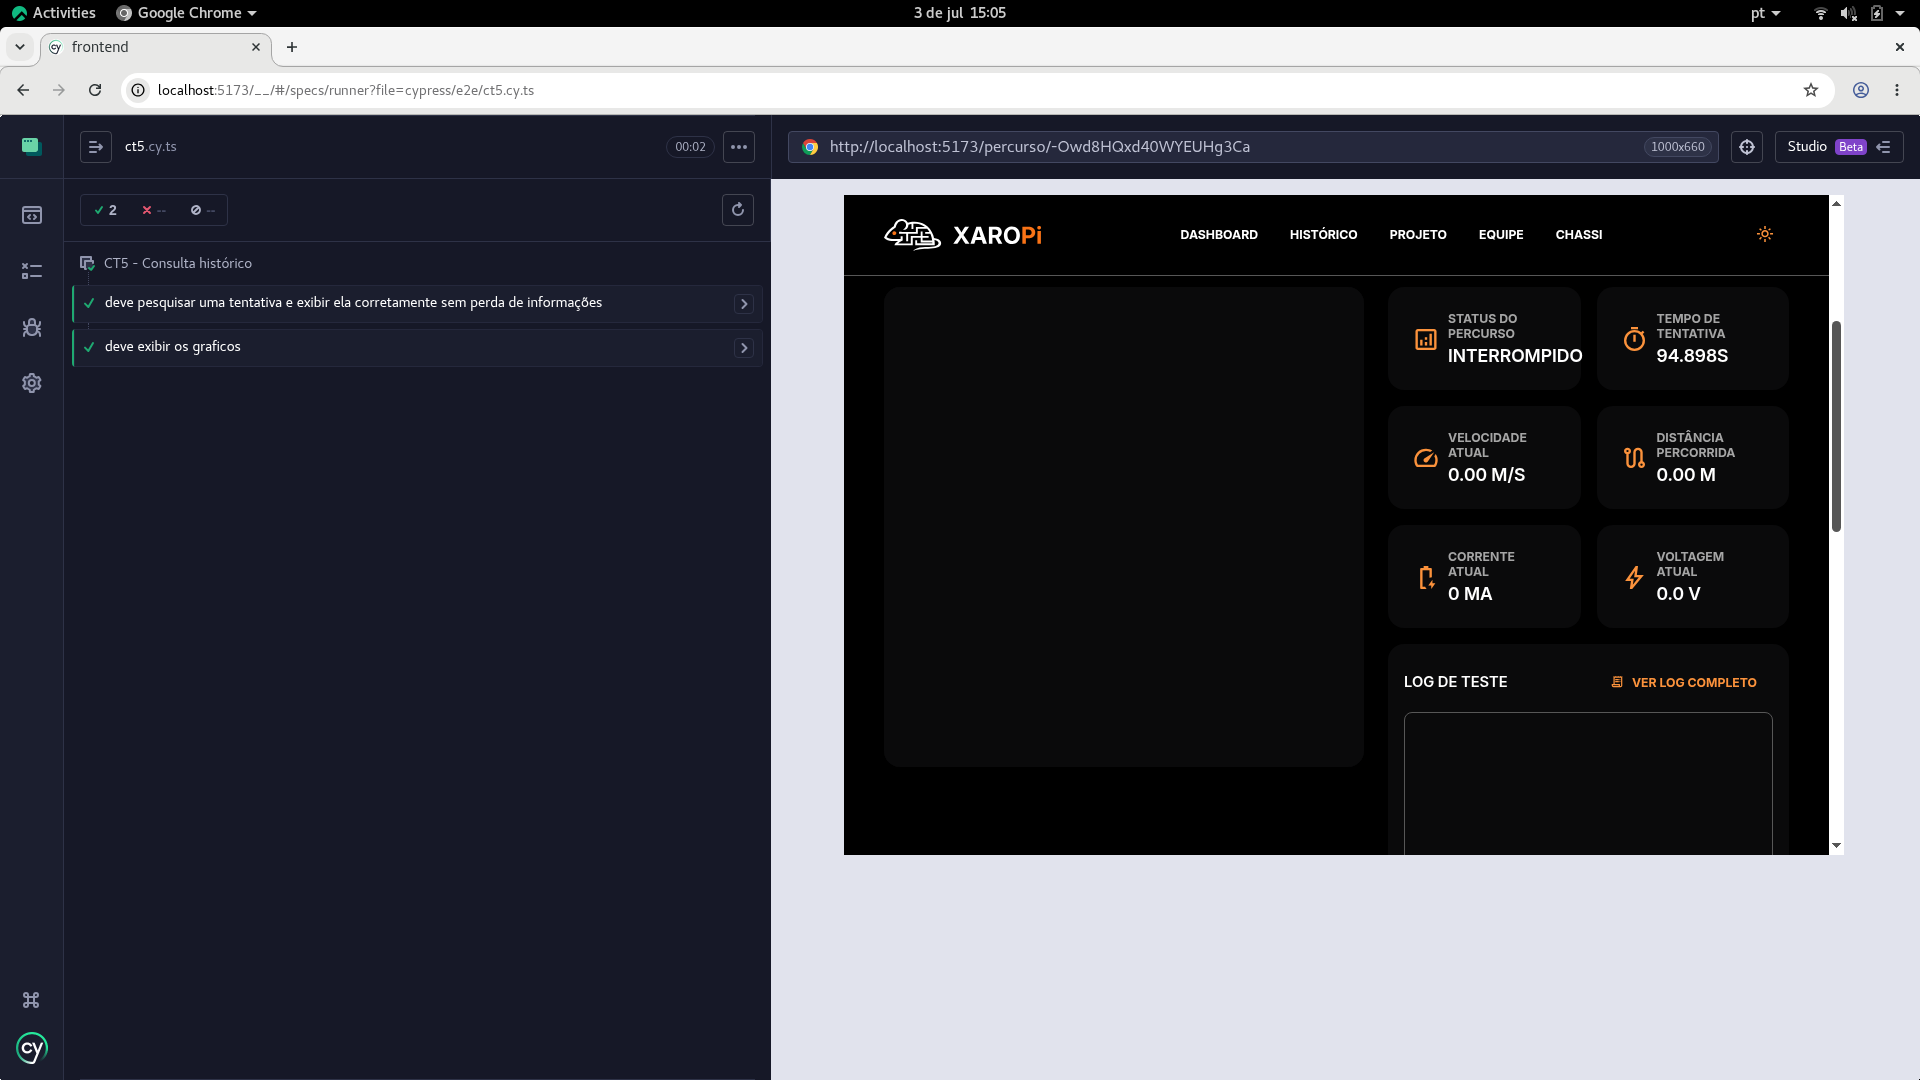
\includegraphics[width=0.9\textwidth]{figuras/software/ct5_cypress.png}
    \caption{Execução do Caso de Teste 05 aprovada no Cypress Runner.}
    \label{fig:ct5_cypress}
\end{figure}

\subsection{Testes de integração}

Os testes de integração tiveram como foco principal validar os \textit{endpoints} da API e sua correta orquestração com a camada de serviços responsáveis pela comunicação e persistência de dados no Firebase Realtime Database.

Para a realização das chamadas, utilizou-se a biblioteca \textit{Supertest}, que simula requisições HTTP e avalia os códigos de status e corpos de resposta. A suíte de testes contemplou o fluxo completo de gerenciamento de corridas e telemetria:

\begin{itemize}
    \item \textbf{GET / (Healthcheck):} Validação da disponibilidade e tempo de resposta da API.
    \item \textbf{POST /telemetria:} Validação do recebimento do \textit{payload} estruturado pelo robô e do acionamento do serviço de salvamento.
    \item \textbf{GET /corridas:} Validação da recuperação, estruturação e formatação dos dados provindos do banco de dados.
    \item \textbf{DELETE /corridas/:id:} Validação da rotina de remoção de registros.
\end{itemize}

Durante a validação, devido a restrições rigorosas de rede no ambiente de desenvolvimento Linux (isolamento provocado por contêineres Flatpak), a conexão externa direta aos servidores do Google Cloud sofreu bloqueios operacionais, falhas de \textit{timeout} e \textit{Gaxios Error}. 

Para contornar essa limitação de infraestrutura sem comprometer a validação da arquitetura, aplicou-se a técnica de \textit{Provider Override} suportada nativamente pelo NestJS. Os serviços de conexão direta, \texttt{FirebaseService} e \texttt{AppService}, foram interceptados e mockados com respostas controladas. 

Essa abordagem atesta que os controladores, as rotas e o sistema de injeção de dependências estão perfeitamente integrados e capazes de processar os dados adequadamente até a fronteira final com o banco de dados. Como ilustrado na figura \ref{fig:integracao_back}, a bateria de testes foi aprovada com sucesso.

\begin{figure}[H]
    \centering
    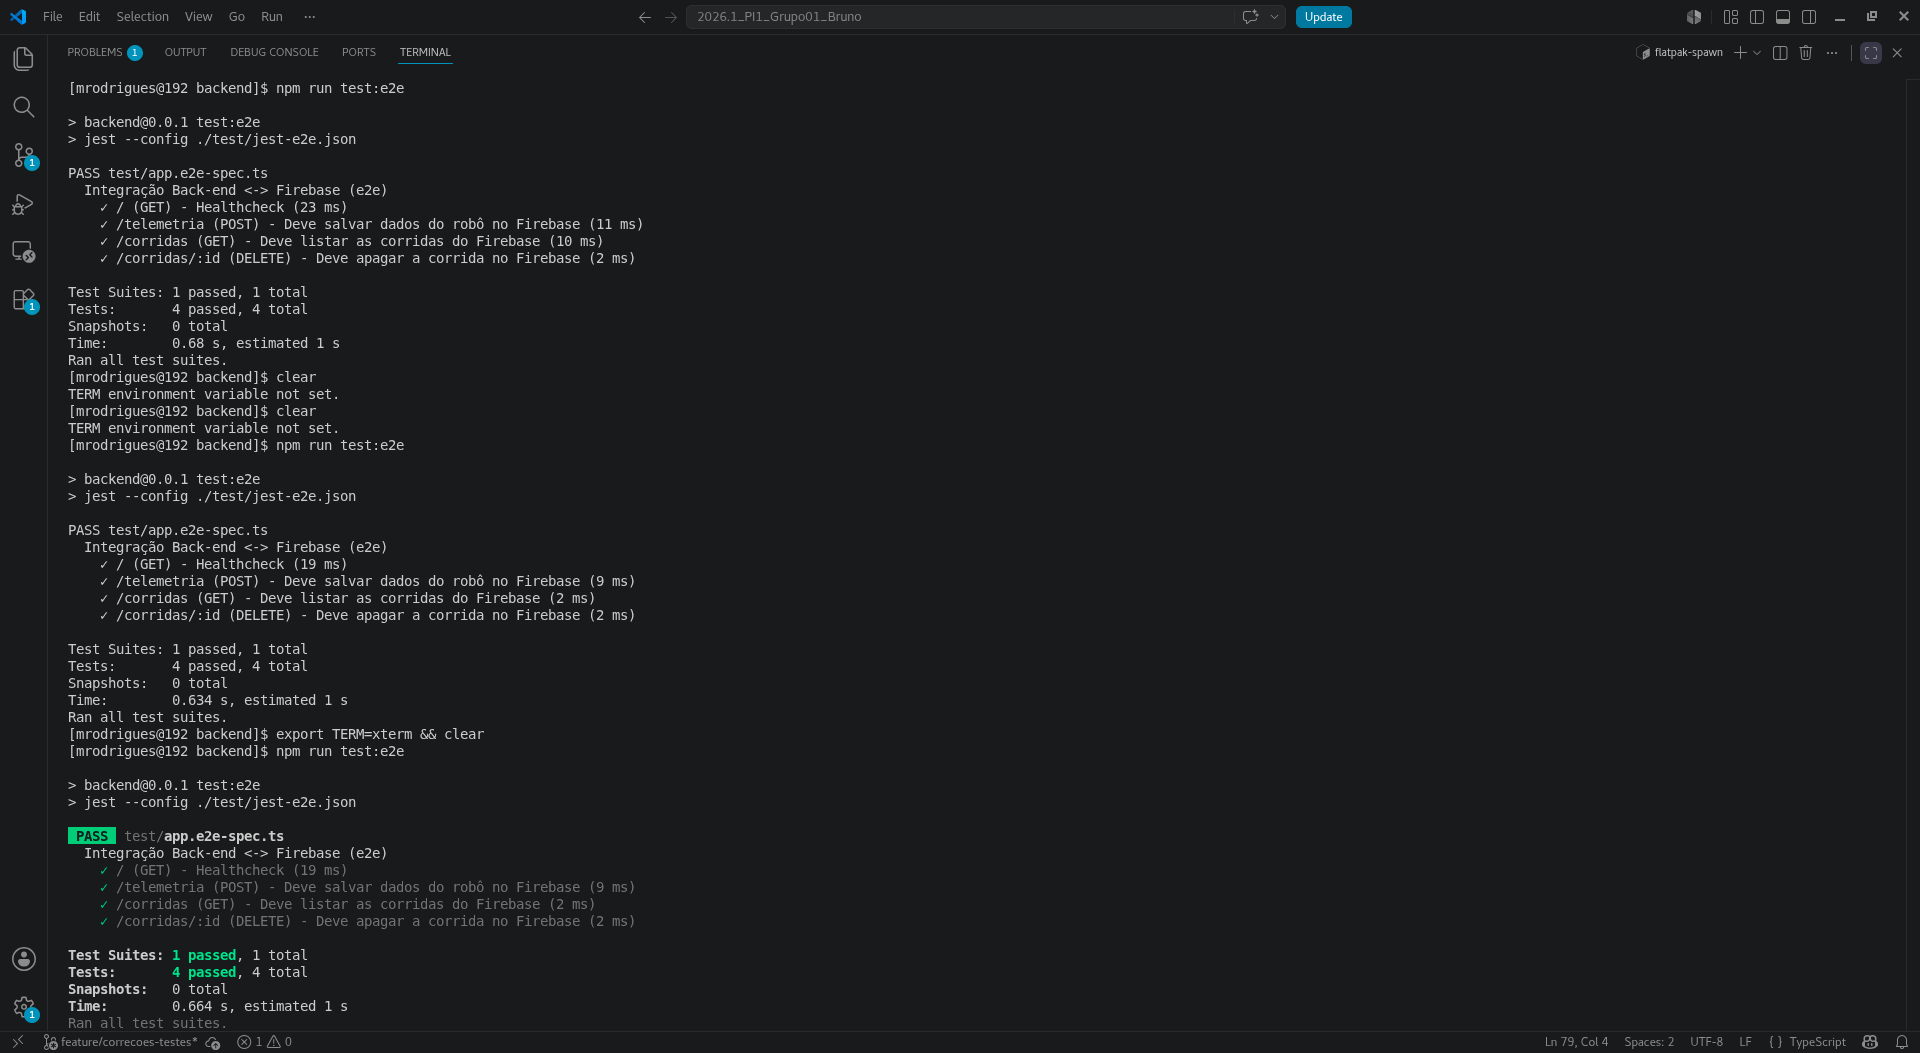
\includegraphics[width=0.7\textwidth]{figuras/software/testeIntegracao.png} 
    \captionsetup{font=footnotesize}
    \caption{Relatório de aprovação dos testes de integração da API (Supertest).}
    \label{fig:integracao_back}
\end{figure}

Além dos testes via \textit{Supertest} sobre os endpoints REST, foi conduzido um teste de integração da camada de comunicação em tempo real, responsável pela troca de telemetria entre o firmware do robô e o backend. Diferentemente dos testes anteriores, essa validação foi executada com o hardware físico conectado à rede \textit{Access Point} da ESP32, permitindo observar o comportamento real do protocolo \textit{Socket.IO} nas duas pontas da comunicação.

Do lado do servidor, o \texttt{TelemetryGateway} foi instrumentado com um sistema de \textit{logging} detalhado, capaz de registrar cada etapa do ciclo de vida da conexão: o recebimento do \textit{handshake} (incluindo parâmetros de \textit{query} como \texttt{role} e endereço IP de origem), a identificação do cliente como firmware, o envio do evento de confirmação \texttt{firmware\_ack} e a propagação do evento \texttt{firmware\_status} para a sala dos clientes \textit{frontend}. Como ilustrado na figura \ref{fig:integracao_ws_backend}, o servidor inicializa corretamente todos os \textit{gateways} e rotas antes de identificar e confirmar a conexão da placa (\texttt{socket.id=VadC7H4PxRelRcUtAAAB}), validando o correto funcionamento da inicialização da aplicação NestJS e do módulo de \textit{WebSockets}.

Do lado do firmware, o monitor serial da ESP32 confirma a recepção do evento de confirmação enviado pelo backend, registrando a mensagem \texttt{[IO] CONECTADO!} seguida do \textit{payload} \texttt{firmware\_ack} com o \textit{status} \texttt{"conectado"} e o respectivo \textit{timestamp}, conforme apresentado na figura \ref{fig:integracao_ws_firmware}. Esse resultado comprova que o protocolo de conexão implementado é bidirecional e íntegro: o backend reconhece e confirma a placa, e a placa recebe e interpreta corretamente essa confirmação, validando de ponta a ponta a integração entre o firmware embarcado e o serviço de telemetria em tempo real.

\begin{figure}[H]figuras/testeIntegracaoWebSocketFirmware.png
    \centering
    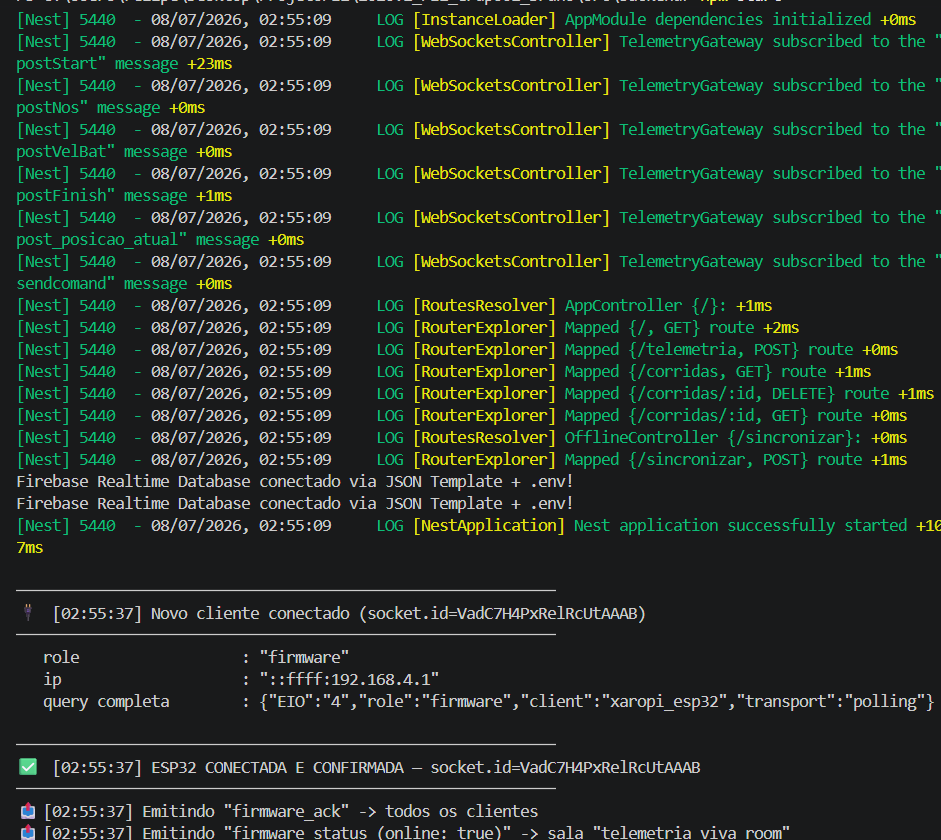
\includegraphics[width=0.7\textwidth]{figuras/testeIntegracaoWebSocketFirmware.png} 
    \captionsetup{font=footnotesize}
    \caption{Logs do backend NestJS durante a inicialização e a conexão da ESP32 via WebSocket.}
    \label{fig:integracao_ws_backend}
\end{figure}

\begin{figure}[H]
    \centering
    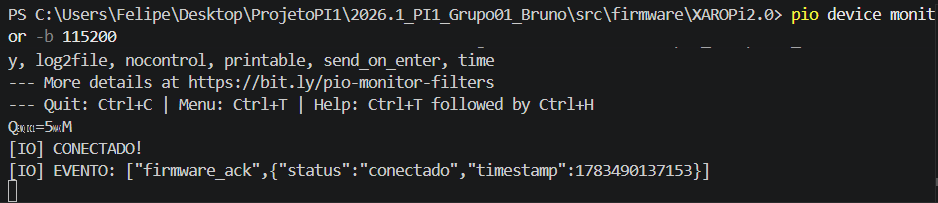
\includegraphics[width=0.7\textwidth]{figuras/testeIntegracaoWebSocketBackend.png} 
    \captionsetup{font=footnotesize}
    \caption{Monitor serial da ESP32 confirmando o recebimento do evento \texttt{firmware\_ack}.}
    \label{fig:integracao_ws_firmware}
\end{figure}
\chapter{Lições Aprendidas}

Esta seção tem como objetivo documentar as lições aprendidas ao longo do desenvolvimento do projeto do micromouse, de forma a consolidar os conhecimentos adquiridos, reconhecer os acertos da equipe e identificar os pontos passíveis de melhoria.

\section{Análise SWOT}

A fim de consolidar as lições aprendidas ao longo do desenvolvimento do micromouse, realizou-se uma análise SWOT do produto, contemplando os fatores internos (pontos fortes e fracos da equipe e do projeto) e os fatores externos (oportunidades e ameaças relacionadas ao contexto do desenvolvimento). A Tabela~\ref{tab:swot} sintetiza os principais pontos identificados pela equipe.

\begin{table}[H]
\centering
\footnotesize
\caption{Análise SWOT do produto.}
\begin{tabular}{|c|c|c|} \hline
 & \textbf{Pontos fortes} & \textbf{Pontos fracos}  \\ \hline 
{\parbox{0.1\textwidth}{ \textbf{Fatores \\ internos}}}  &
{\parbox{0.4\textwidth}{ Forças: 
\begin{itemize}
    \item Chassi leve, com bom desempenho geral
    \item Bateria eficiente e boa autonomia
    \item Lógica planejada previamente, agilizando diagnóstico de erros
    \item Inerciômetro como redundância, mitigando falha de encoder
    \item Experiência prévia da equipe em tecnologias específicas
    \item Arquitetura em React.js modular e escalável
    \item Comunicação em tempo real via WebSocket
    \item Extras de valor agregado, como carrinho em 3D
    \item Agilidade no dimensionamento da alimentação elétrica
\end{itemize}}}
&
{\parbox{0.4\textwidth}{ Fraquezas:
\begin{itemize}
    \item Largura/formato do chassi maior que o ideal, dificultando manobras nas curvas
    \item Queima de componentes durante o processo
    \item Aumento do orçamento previsto devido à reposição dos componentes danificados
    \item Eletrônica mais sensível devido ao uso de jumpers em placa perfurada
    \item Banco de dados dependente de conexão à internet, exigindo solução de backup offline
    \item Predominância de testes isolados em detrimento de testes de integração, gerando imprevistos na integração final
\end{itemize}}}
\\ \hline

{\parbox{0.1\textwidth}{ \textbf{Fatores \\ externos}}}  &
{\parbox{0.4\textwidth}{ Oportunidades:
\begin{itemize}
    \item Reaproveitamento do chassi, algoritmo de navegação e sistema de energia como base para outros projetos acadêmicos, TCCs ou iniciação científica
    \item Adaptação dos módulos desenvolvidos (gerenciamento de energia, navegação) para outros robôs móveis, como VANTs ou rovers
\end{itemize}}}
&
{\parbox{0.4\textwidth}{ Ameaças:
\begin{itemize}
    \item Prazo apertado devido a imprevistos técnicos
    \item Falhas pequenas acumuladas dificultando diagnóstico na integração
    \item Alto escopo de entregas em curto prazo
    \item Dificuldade em organizar o GitHub em relação à EAP
    \item Demora na integração com hardware, atrasando a telemetria
\end{itemize}}}
\\ \hline
\end{tabular}
\label{tab:swot}
\end{table}


\section{Planejado x realizado}

\subsection{Prazos}

\subsection{Orçamento}

No início do projeto, foi pensado um orçamento máximo de 1.000 reais. A intenção era trabalhar com um valor abaixo do limite, porém, devido ao caráter iterativo do projeto, surgiram custos adicionais, já que diversas soluções precisaram ser testadas e ajustadas até chegar ao resultado desejado. Por outro lado, no início do desenvolvimento, a equipe conseguiu algumas peças emprestadas, o que proporcionou uma maior folga orçamentária. Dessa forma, mesmo com os imprevistos, o valor total permaneceu dentro do limite estabelecido, fechando em 853,88 reais, sendo que a maior parte do investimento foi direcionada aos componentes eletrônicos.

\subsection{Escopo}

No que diz respeito ao escopo do projeto, os objetivos definidos foram majoritariamente cumpridos e o micromouse foi construído conforme planejado, 
integrando todas as áreas devidamente. Porém, alguns componentes e funcionalidades não foram incorporados à versão final do projeto, na área de hardware, por exemplo,
o giroscópio MPU-6050 foi removido devido ao ruído eletromagnético que comprometeu a leitura dos valores. Além disso, a capacidade de medição de direção 
da rotação dos motores foi comprometida e o fio C2 dos encoders não foi utilizado. Em firmware, os switches de seleção e o botão de liga/desliga não foram integrados ao sistema devido
ao espaço limitado da placa.


\section{Projeto}

A partir da experiência acumulada durante as etapas de desenvolvimento, integração e testes do micromouse, foram identificados os principais pontos fortes e fracos do projeto, descritos a seguir.

\subsection{Pontos Fortes}

\begin{enumerate}
    \item Chassi leve e de montagem simples, facilitando ajustes e manutenção ao longo do projeto.
    \item Uso do inerciômetro como redundância, essencial diante da falha em um dos encoders.
    \item Arquitetura em React.js e comunicação via WebSocket garantiram um frontend modular e responsivo.
    \item Experiência prévia da equipe em tecnologias específicas acelerou o desenvolvimento geral.
\end{enumerate}

\subsection{Pontos fracos}

\begin{enumerate}
    \item Formato do chassi dificultou manobras nas curvas do labirinto.
    \item Queima de componentes durante o processo, elevando o orçamento previsto do projeto.
    \item Predomínio de testes isolados sobre testes de integração, gerando imprevistos na integração final.
    \item Engajamento desigual entre os membros da equipe, dificultando o cumprimento dos prazos.
\end{enumerate}

\section{Recomendações para projetos futuros}

\begin{enumerate}
    \item Priorizar entregas críticas do caminho principal antes de 
    funcionalidades secundárias, evitando acúmulo de pendências próximo 
    ao prazo final.
    
    \item Melhorar a comunicação entre as subequipes, estabelecendo 
    reuniões regulares de alinhamento para reduzir retrabalho causado 
    por decisões tomadas de forma isolada.
    
    \item Concluir cada entrega de forma sólida antes de avançar para 
    a próxima, evitando retrabalho comprometer a integração final do sistema.
    
    \item Adotar revisão em dupla para todas as entregas técnicas, 
    reduzindo erros simples e aumentando a qualidade do código e da 
    documentação produzidos.
\end{enumerate}

\section{Desempenho dos fornecedores}


Esta seção apresenta uma avaliação dos fornecedores utilizados ao longo do desenvolvimento do projeto, classificados conforme o desempenho apresentado em relação ao esperado pela equipe.

\subsection{Fornecedores com desempenho acima do esperado}

Fornecedores que a equipe certamente convidaria para um próximo projeto.

\begin{itemize}
    \item \textbf{HU Infinito} -- Ampla variedade de produtos, atendimento de qualidade e entregas sempre pontuais.
    \item \textbf{SIA Parafusos e Ferramentas} -- Atendimento rápido, apesar de nem todos os modelos necessários estarem disponíveis em estoque.
\end{itemize}

\subsection{Fornecedores com desempenho conforme esperado}

Fornecedores que a equipe provavelmente convidaria para um próximo projeto.

\begin{itemize}
    \item \textbf{RoboCore} -- Pedido entregue com boa qualidade, porém com atraso em relação ao prazo combinado.
\end{itemize}

\subsection{Fornecedores com desempenho abaixo do esperado}

Fornecedores que a equipe não convidaria para um próximo projeto.

\begin{itemize}
    \item \textbf{Casa dos Parafusos} -- Variedade adequada de produtos, porém atendimento demorado.
    \item \textbf{Dr. Eletrônico} -- Entrega não prática e atendimento confuso durante o processo de compra.
\end{itemize}


% Resolvi não pagar os comentarios abaixo por enquanto para fins de consulta


% \chapter{Lições Aprendidas}

% \textcolor{red}{Documentar as lições aprendidas de modo a aperfeiçoar os processos e evitar que os erros e problemas encontrados se repitam em futuros projetos.}

% \section{Análise SWOT}

% \textcolor{red}{A análise SWOT (\textit{Strengths}, \textit{Weaknesses}, \textit{Opportunities}, \textit{Threats}) é usada para identificar os pontos fortes e fracos do produto, e as principais oportunidades e ameaças normalmente associadas aos pontos fortes e fracos identificados. Preencha a Tabela \ref{tab:swot} de forma correspondente.}

% \begin{table}[ht]
% % \label{tab:swot}
% \centering
% \caption{Análise SWOT do produto.}
% \begin{tabular}{|c|c|c|} \hline
%  & \textbf{Pontos fortes} & \textbf{Pontos fracos}  \\ \hline 
%     {\parbox{0.1\textwidth}{ \textbf{Fatores \\ internos}}}  &
%     {\parbox{0.4\textwidth}{ Forças: 
%         \\ \textcolor{red}{Descreva seus diferenciais competitivos: aquilo que faz de você melhor que seus concorrentes.}
%         \begin{itemize}
%             \item Lorem ipsum
%             \item Lorem ipsum
%         \end{itemize} }} & 
%     {\parbox{0.4\textwidth}{ Fraquezas:
%         \\ \textcolor{red}{Descreva suas principais deficiências: aquilo que faz de você pior que seus concorrentes, e pontos a serem melhorados ou revistos.}
%         \begin{itemize}
%             \item Lorem ipsum
%             \item Lorem ipsum
%         \end{itemize} }}\\ \hline
%     {\parbox{0.1\textwidth}{ \textbf{Fatores \\ externos}}}  &
%     {\parbox{0.4\textwidth}{ Oportunidades:
%         \\ \textcolor{red}{Descreva as principais oportunidades identificadas: eventos potenciais que podem gerar grandes benefícios.}
%         \begin{itemize}
%             \item Lorem ipsum 
%             \item Lorem ipsum
%         \end{itemize} }} & 
%     {\parbox{0.4\textwidth}{ Ameaças:
%         \\ \textcolor{red}{Descreva as principais ameaças identificadas: eventos potenciais que podem causar um grande estrago ao seu negócio.}
%         \begin{itemize}
%             \item Lorem ipsum 
%             \item Lorem ipsum
%         \end{itemize} }}\\ \hline
% \end{tabular}
% \label{tab:swot}
% \end{table}


% \section{Planejado x realizado}
% \subsection{Objetivos}
% \textcolor{red}{Os objetivos foram alcançados? Responda as questões e comente os pontos mais relevantes – até 700 caracteres, considerando os espaços.}
% \subsection{Prazos}
% \textcolor{red}{O projeto foi entregue dentro do prazo? Responda as questões e comente os pontos mais relevantes – até 700 caracteres, considerando os espaços.}
% \subsection{Orçamento}
% \textcolor{red}{O projeto foi entregue dentro do orçamento? Responda as questões e comente os pontos mais relevantes – até 700 caracteres, considerando os espaços.}
% \subsection{Escopo}
% \textcolor{red}{O  projeto atendeu ao escopo? Responda as questões e comente os pontos mais relevantes – até 700 caracteres, considerando os espaços.}


% \section{Projeto}
% \textcolor{red}{Comente os pontos mais relevantes a serem aperfeiçoados ou adotados em próximos projetos.}
% \subsection{Pontos fortes}
% \begin{enumerate}
% 	\item \textcolor{red}{Até 200 caracteres, considerando os espaços.}
% 	\item \textcolor{red}{Até 200 caracteres, considerando os espaços.}
% 	\item \textcolor{red}{Até 200 caracteres, considerando os espaços.}
% 	\item \textcolor{red}{Até 200 caracteres, considerando os espaços.}
% \end{enumerate}
% \subsection{Pontos fracos}
% \begin{enumerate}
% 	\item \textcolor{red}{Até 200 caracteres, considerando os espaços.}
% 	\item \textcolor{red}{Até 200 caracteres, considerando os espaços.}
% 	\item \textcolor{red}{Até 200 caracteres, considerando os espaços.}
% 	\item \textcolor{red}{Até 200 caracteres, considerando os espaços.}
% \end{enumerate}

% \section{Recomendações para projetos futuros}

% \begin{enumerate}
% 	\item \textcolor{red}{Até 200 caracteres, considerando os espaços.}
% 	\item \textcolor{red}{Até 200 caracteres, considerando os espaços.}
% 	\item \textcolor{red}{Até 200 caracteres, considerando os espaços.}
% 	\item \textcolor{red}{Até 200 caracteres, considerando os espaços.}
% \end{enumerate}

% \section{Questões em aberto}

% \textcolor{red}{Usar caso haja alguma questão pendente em relação às entregas do projeto (Ex.: Requisitos não entregues, melhoria na programação do software, troca de sensores, entre outros.}

% \begin{enumerate}
% 	\item \textcolor{red}{Até 200 caracteres, considerando os espaços.}
% 	\item \textcolor{red}{Até 200 caracteres, considerando os espaços.}
% 	\item \textcolor{red}{Até 200 caracteres, considerando os espaços.}
% 	\item \textcolor{red}{Até 200 caracteres, considerando os espaços.}
% \end{enumerate}

% \section{Desempenho dos fornecedores}

% \subsection{Fornecedores com desempenho acima do esperado}
% \textcolor{red}{Fornecedores que você certamente convidaria para um próximo projeto. Citar AAAA – justificativa. Até 200 caracteres, considerando os espaços.}

% \subsection{Fornecedores com desempenho conforme esperado}
% \textcolor{red}{Fornecedores que você provavelmente convidaria para um próximo projeto. Citar AAAA – justificativa. Até 200 caracteres, considerando os espaços.}

% \subsection{Fornecedores com desempenho abaixo do esperado}
% \textcolor{red}{Fornecedores que você não convidaria para um próximo projeto. Citar AAAA – justificativa. Até 200 caracteres, considerando os espaços.}

\bookmarksetup{startatroot}

\postextual

\bibliography{bibliografia}
\begin{apendicesenv}
% \partapendices

\chapter{DESENHO TÉCNICO DO CHASSI}

Este apêndice apresenta o desenho técnico do chassi desenvolvido para o projeto, contendo dimensões e vistas estruturais.

\begin{itemize}
    \item Projeto: Chassi do protótipo
    \item Autor: Samara Sardinha Sousa
    \item Escala: 2:3
    \item Unidade: milímetros (mm)
\end{itemize}

\begin{figure}[H]
    \centering
    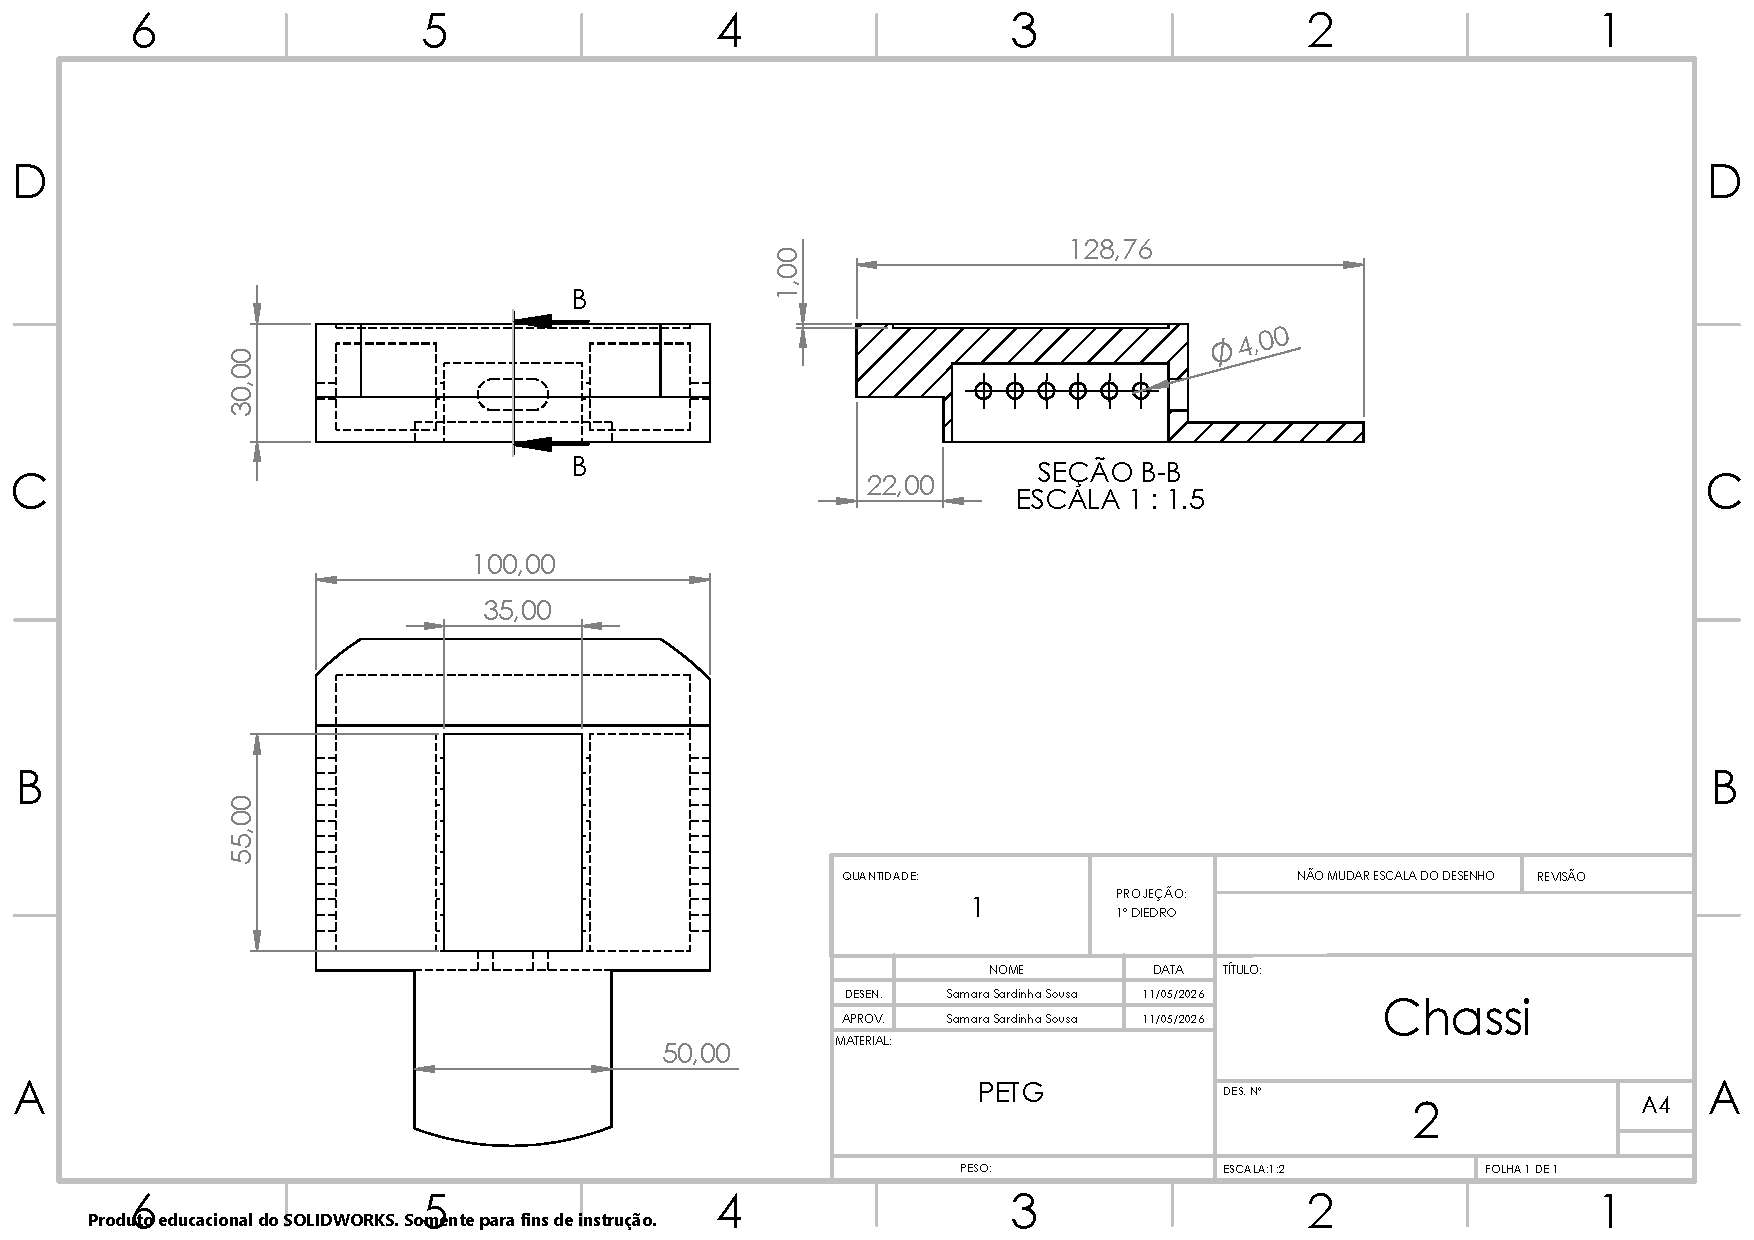
\includegraphics[width=1\linewidth]{figuras/chassi.pdf}
    \caption{Desenho técnico do chassi com vistas superior, lateral e frontal}
    \label{fig:chassi}
\end{figure}


\chapter{Segundo Apêndice}
\textcolor{red}{Apêndices e anexos são materiais complementares ao texto que só devem ser incluídos quando forem imprescindíveis à compreensão deste:}

\textcolor{red}{
\begin{itemize}
    \item Apêndices são textos elaborados pelo autor a fim de complementar sua argumentação.
    \item Anexos são os documentos não elaborados pelo autor, que servem de fundamentação, comprovação ou ilustração, como mapas, leis, estatutos etc.
\end{itemize}}

\textcolor{red}{\textbf{Texto do segundo apêndice.}}
 
\chapter{Terceiro Apêndice}
\begin{figure}[H]
    \centering
    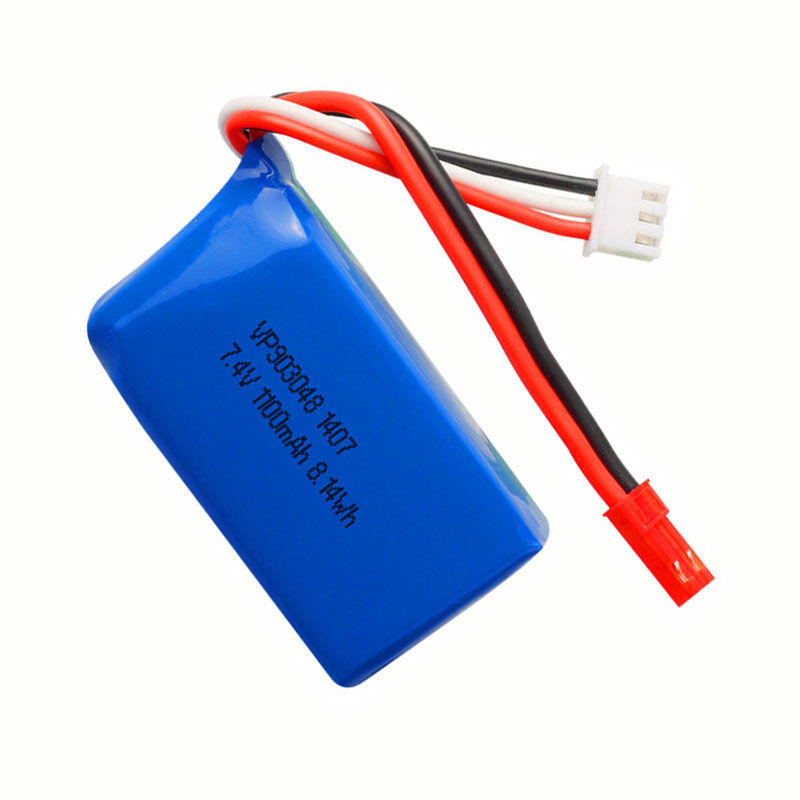
\includegraphics[width=0.6\textwidth]{figuras/imagembateria.png}
    \captionsetup{font=footnotesize}
    \caption{Imagem ilustrativa da bateria selecionada.}
\end{figure}

\end{apendicesenv}
\begin{anexosenv}
% \partanexos

\chapter{BATERIA}

Este anexo apresenta uma imagem ilustrativa da bateria selecionada para o projeto.

\begin{figure}[H]
    \centering
    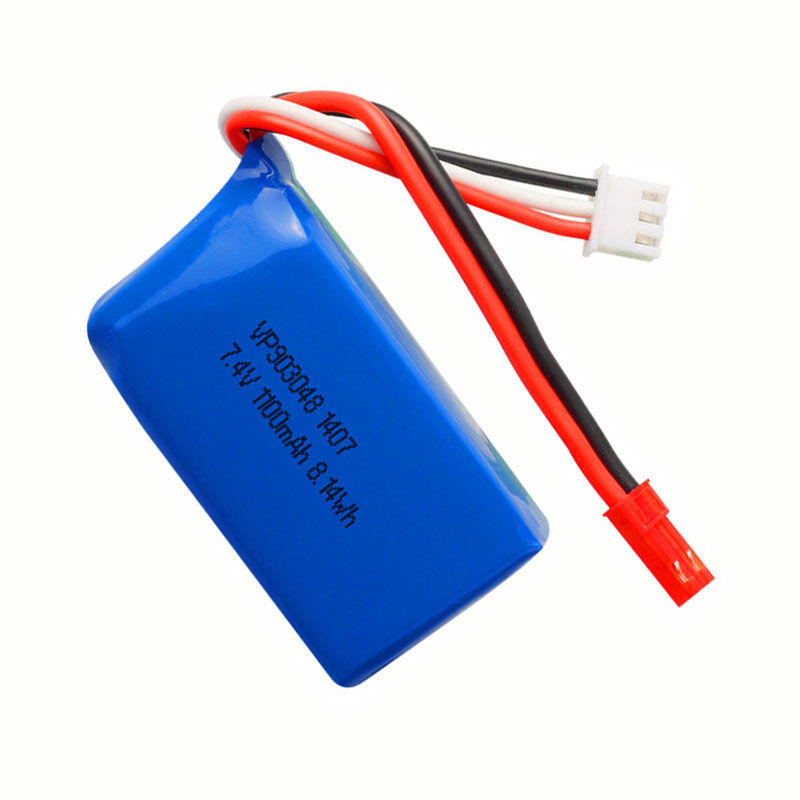
\includegraphics[width=0.6\textwidth]{figuras/imagembateria.png}
    \captionsetup{font=footnotesize}
    \caption{Imagem ilustrativa da bateria selecionada.}
\end{figure}

% \textcolor{red}{Apêndices e anexos são materiais complementares ao texto que só devem ser incluídos quando forem imprescindíveis à compreensão deste:}

% \textcolor{red}{
% \begin{itemize}
%     \item Apêndices são textos elaborados pelo autor a fim de complementar sua argumentação.
%     \item Anexos são os documentos não elaborados pelo autor, que servem de fundamentação, comprovação ou ilustração, como mapas, leis, estatutos etc.
% \end{itemize}}
% \textcolor{red}{\textbf{Texto do primeiro anexo.}}

% \chapter{Segundo Anexo}
% \textcolor{red}{Apêndices e anexos são materiais complementares ao texto que só devem ser incluídos quando forem imprescindíveis à compreensão deste:}

% \textcolor{red}{
% \begin{itemize}
%     \item Apêndices são textos elaborados pelo autor a fim de complementar sua argumentação.
%     \item Anexos são os documentos não elaborados pelo autor, que servem de fundamentação, comprovação ou ilustração, como mapas, leis, estatutos etc.
% \end{itemize}}
% \textcolor{red}{\textbf{Texto do segundo anexo.}}

% \begin{figure}[htpb]
% \centering
% 
\includegraphics[width=\textwidth]{figuras/fga.png}
% \caption{Figura do Anexo 2.}
% \label{fig:fig_anexo}
% \end{figure}

\end{anexosenv}

\printindex

\end{document}
